\documentclass[10pt,a4paper]{article}
\usepackage[utf8]{inputenc}
\usepackage[T1]{fontenc}
\usepackage[spanish,es-nodecimaldot]{babel}
\usepackage[margin=2cm]{geometry}
\usepackage{graphicx}
\usepackage{pdfpages}
\usepackage{amsmath}
\usepackage{float}
\usepackage{longtable}
\usepackage{microtype}
\usepackage[colorlinks=true,urlcolor=blue,linkcolor=blue]{hyperref}
\setlength{\parindent}{0pt}
\setlength{\parskip}{5pt}
\usepackage{booktabs}
\begin{document}
% PORTADA_INSTITUCIONAL_INICIO
\begin{titlepage}
\centering
\vspace*{0.5cm}
\vspace{0.8cm}
{\huge\bfseries Cuenca del río La Vieja\par}
\vspace{0.4cm}
{\Large Exploración hidroclimática mensual\par}
\vspace{0.5cm}
{\large Curso: Hidrología\par}
\vspace{0.6cm}
{\large\bfseries Profesor\par}
{\large Carlos David Hoyos Ortiz\par}
\vspace{0.9cm}
{\large\bfseries Integrantes\par}
\vspace{0.4cm}
{\large Marcos Correal Suarez\par
Andrea Carolina Vergara Tenorio\par
Mariana Campuzano Tobón\par}
\vspace{0.3cm}
{\large Ingeniería Civil\par}
\vspace{0.9cm}
\includegraphics[width=3.7cm,trim=850bp 230bp 820bp 150bp,clip]{figuras/escudos_unal_oficial.jpg}\par
\vspace{0.5cm}
{\Large\bfseries Universidad Nacional de Colombia\par}
\vspace{0.2cm}
{\large Sede Medellín\par Facultad de Minas\par}
\vfill
{\large Medellín, Colombia\par 2026\par}
\vspace*{0.6cm}
\end{titlepage}
% PORTADA_INSTITUCIONAL_FIN

\tableofcontents
\clearpage
\section*{Introducción}
La variabilidad de la precipitación y del caudal condiciona la disponibilidad de agua y la ocurrencia de periodos secos y crecientes en las cuencas andinas. En el río La Vieja, el contraste entre las zonas montañosas y los sectores bajos del valle, junto con la variabilidad del clima tropical, motiva estudiar cómo cambia la respuesta hidrológica a lo largo del año y entre años.

Este informe analiza la cuenca del río La Vieja hasta la estación Cartago mediante series mensuales de precipitación, caudal y temperatura. Se examinan el ciclo anual, las distribuciones y los valores extremos; se comparan CHIRPS e IMERG y se evalúan modelos estadísticos de lluvia–caudal y tendencias temporales. El análisis se complementa con la selección de campos oceánicos y atmosféricos globales para estudiar asociaciones climáticas. Las relaciones estadísticas se interpretan considerando la cobertura de los datos, la topografía y las diferencias entre las fuentes.
\section*{Metodología}
La delimitación de la cuenca y las series hidrológicas de referencia proceden de CAMELS-COL. La precipitación CHIRPS se analiza como promedio de cuenca y el caudal corresponde a Cartago (IDEAM 26127040). IMERG Final Run V07B y la temperatura ERA5-Land se ponderan según el área de intersección de sus celdas con la cuenca. Estos productos representan estimaciones espaciales distintas de una observación pluviométrica puntual.

El registro hidrológico abarca 1981–2022. Los acumulados de lluvia y las medias de caudal se calculan únicamente para meses con todos sus días válidos: se conservan 485 de 504 meses. La comparación entre CHIRPS, IMERG y caudal utiliza 285 meses simultáneos de 1998–2022. Los vacíos se mantienen sin relleno. Las diferencias estacionales se examinan mediante climatologías y anomalías mensuales; la evaluación de modelos distingue el periodo de ajuste de la reserva temporal. Los criterios y las incertidumbres específicos se documentan junto a cada análisis.
\clearpage
\section*{Área de estudio: cuenca del río La Vieja}
La cuenca del río La Vieja se localiza en el centro-occidente de Colombia, en la región del Eje Cafetero, y comprende territorios de Quindío, Risaralda y Valle del Cauca. Su red hidrográfica conecta las vertientes de la cordillera Central con los sectores bajos próximos a Cartago. El río La Vieja se forma por la confluencia de los ríos Quindío y Barragán y desemboca en el río Cauca, de cuya red de drenaje es tributario.

El área de estudio corresponde a la cuenca aguas arriba de la estación Cartago (IDEAM 26127040), delimitada en CAMELS-COL, con una superficie de 2.797,19 km$^2$. Esta delimitación define el área sobre la que se promedian los productos de precipitación y temperatura y el territorio cuyos aportes se integran en el caudal observado. Su extensión no debe confundirse con la cuenca administrativa completa descrita en los instrumentos de ordenamiento ambiental.

El relieve presenta un contraste marcado entre las zonas altas de la cordillera y el sector de salida hacia Cartago, con elevaciones del orden de 900 a 4.800 m en la información topográfica analizada. Esta heterogeneidad es relevante para la distribución espacial de la lluvia y la temperatura y para el tránsito y almacenamiento del agua. Las series de cuenca muestran un ciclo de precipitación bimodal, con máximos alrededor de abril–mayo y octubre–noviembre. Por ello, la interpretación de la relación lluvia–caudal distingue el ciclo estacional compartido de las variaciones entre años.
\begin{figure}[H]\centering\includegraphics[width=.82\linewidth]{figuras/mapa_cuenca_estaciones_geografico.pdf}\caption{Localización de la cuenca hasta Cartago y estaciones de lluvia inventariadas. Base: \copyright\ OpenStreetMap contributors; delimitación: CAMELS-COL; estaciones: catálogo IDEAM.}\end{figure}
Fuentes de contexto: \href{https://crq.gov.co/wp-content/uploads/2021/03/PGARQUINDIO2020-2039.pdf}{CRQ, Plan de Gestión Ambiental Regional 2020–2039}; \href{https://www.cvc.gov.co/sites/default/files/2018-09/Balance_La_Vieja_1.pdf}{CVC, Balance oferta–demanda de agua: río La Vieja}; \href{https://doi.org/10.5281/zenodo.18794895}{CAMELS-COL}.
\clearpage
\subsubsection*{Mapas de la cuenca y topografía}
\subsubsection*{Delimitación y red terrestre inventariada}
Se utiliza el polígono CAMELS transformado a WGS84 y la ubicación de Cartago del
catálogo IDEAM. Los 92 puntos son estaciones activas de categorías que miden
lluvia; no se ha verificado la continuidad de sus series.
\begin{figure}[H]\centering
\includegraphics[width=.72\linewidth]{figuras/mapa_cuenca_estaciones.pdf}
\caption{Cuenca La Vieja hasta Cartago y estaciones terrestres inventariadas.}
\end{figure}

\subsubsection*{Modelo de elevación descargado}
Se descargó Copernicus DEM GLO-30 público, mosaico N04/W076, y se recortó al
polígono. Se conserva el GeoTIFF a resolución nominal de unos 30 m; la figura
usa una malla reducida por promedio. Es un modelo de superficie (DSM), que puede
incluir vegetación y construcciones, no un modelo de terreno desnudo.
\begin{figure}[H]\centering
\includegraphics[width=.72\linewidth]{figuras/mapa_relieve.pdf}
\caption{Relieve de La Vieja con Copernicus GLO-30. Alturas en metros, EGM2008.}
\end{figure}
El recorte presenta mínimo 908.5 m, media de píxeles 1799.0 m y máximo 4774.2 m. 
CAMELS reporta 940,54, 1826,21 y 4795 m, respectivamente. Las diferencias entre
modelos, máscaras y resolución se documentan y no sustituyen automáticamente los
atributos originales. El DSM no representa cambios durante el periodo 1981--2022.

Fuente: \href{https://doi.org/10.5270/ESA-c5d3d65}{Copernicus DEM} y
\href{https://copernicus-dem-30m.s3.amazonaws.com/readme.html}{distribución pública COG}.

{\footnotesize produced using Copernicus WorldDEM-30 \textcopyright\ DLR e.V.
2010-2014 and \textcopyright\ Airbus Defence and Space GmbH 2014-2018 provided
under COPERNICUS by the European Union and ESA; all rights reserved}

\clearpage
\section{Series mensuales: exploración y validación}

\subsection{Variabilidad temporal de la precipitación y del caudal}
\subsubsection*{Series de precipitación y caudal}

Se analiza la cuenca del río La Vieja hasta la estación Cartago (IDEAM 26127040), con un área CAMELS de 2797,19~km$^2$. El periodo comprende enero de 1981 a diciembre de 2022. Se utiliza precipitación CHIRPS v2 promediada sobre la cuenca y caudal observado según el depósito \href{https://doi.org/10.5281/zenodo.18794895}{CAMELS-COL}.

$P_{L,m}$ es la precipitación de referencia elegida: CHIRPS v2 diario, promediado sobre la cuenca por CAMELS-COL y acumulado a mm/mes. CHIRPS es un producto combinado espacial, no la observación independiente de un único pluviómetro local. $P_{I,m}$ es IMERG Final Run V07 en mm/mes. Para la comparación simultánea de $P_{L,m}$, $P_{I,m}$ y Q se define enero de 1998--diciembre de 2022, con 285 meses completos; los 15 meses sin Q se mantienen como faltantes y no se rellenan.

\subsubsection*{Agregación y tratamiento de faltantes}
La precipitación mensual se obtiene sumando los valores diarios y el caudal mensual promediándolos. Para un mes completo con $n_m$ días:
\[
P_m=\sum_{d\in m}P_d\quad[\mathrm{mm/mes}],\qquad
Q_m=\frac{1}{n_m}\sum_{d\in m}Q_d\quad[\mathrm{m^3/s}].
\]
Se conserva únicamente un mes con el 100\,\% de sus días válidos. El calendario contiene 15\,340 días esperados y 255 ausentes (1,66\,\%). Quedan 485 meses completos de 504; los 19 restantes se mantienen como vacíos. No se rellenan ni prorratean registros y se conservan los extremos.

\begin{figure}[H]
\centering
\includegraphics[width=\linewidth]{figuras/series_mensuales.pdf}
\caption{Precipitación acumulada y caudal medio mensuales de La Vieja--Cartago. Los paneles comparten el eje temporal; las franjas grises indican meses excluidos por días faltantes. Elaboración propia con CAMELS-COL.}
\label{fig:series-mensuales}
\end{figure}

\subsubsection*{Lectura inicial y alcance}
Se observan oscilaciones estacionales y diferencias entre años (figura~\ref{fig:series-mensuales}). El máximo de precipitación mensual ocurre en octubre de 2022 (407,57~mm); el máximo de caudal medio mensual, en noviembre de 2010 (508,77~m$^3$/s). No coinciden, lo que motiva examinar los aportes previos y la respuesta de la cuenca sin atribuir todavía una causa.

\subsubsection*{Meses extremos y contraste cronológico}
Los extremos que deben localizarse en la figura~\ref{fig:series-mensuales} son: agosto de 1982, mínimo de P (24,89~mm); octubre de 2022, máximo de P (407,57~mm); julio de 1992, mínimo de Q (18,37~m$^3$/s) y R (17,59~mm); y noviembre de 2010, máximo de Q (508,77~m$^3$/s) y R (471,45~mm). R es una conversión del caudal a lámina mensual, por lo cual sus extremos son coherentes con los de Q.

Que el máximo de P y el de Q ocurran en meses distintos no indica por sí solo un error: el caudal integra lluvia antecedente, almacenamiento y respuesta de la cuenca. Noviembre de 2010 es un episodio plausible: IDEAM documentó una temporada lluviosa inusitada durante La Niña, con humedad del suelo superior a la usual e inundaciones en las regiones Andina y del Cauca. Los mínimos de 1982 y 1992 también son compatibles con periodos secos asociados a El Niño reportados por IDEAM. Esta interpretación es de plausibilidad, no de causalidad: aún se deben revisar datos diarios, metadatos y cambios de instrumento para descartar un problema de medición.

\subsubsection*{Referencias del contraste climático}
IDEAM (2010). \textit{Boletín diciembre de 2010}. Disponible en \url{https://www.ideam.gov.co/file-download/download/public/6150}.

IDEAM (2006). \textit{La sequía en Colombia}, nota técnica NT\_IDEAM-2006-004.

Esta primera sección presenta las series históricas y la comparación IMERG disponible desde 1998. Las gráficas no demuestran por sí solas tendencias ni causas físicas. El código Python genera la figura vectorial y una versión Plotly con las mismas fechas y valores para su exploración interactiva.\subsubsection*{Temperatura mensual}
Se grafican las medias mensuales de Tmin y Tmax diarias de MSWX incluidas en
CAMELS, no los extremos absolutos del mes. La \textbf{temperatura media es estimada}:
$T_{d,\mathrm{est}}=(T_{d,\min}+T_{d,\max})/2$, seguida del promedio mensual.
No equivale necesariamente a una media de observaciones horarias. Se conservan
485 meses completos por curva y se mantienen los vacíos.
\begin{figure}[H]\centering
\includegraphics[width=\linewidth]{figuras/temperaturas_mensuales.pdf}
\caption{Medias mensuales de Tmin, Tmax y temperatura media estimada de la cuenca.}
\end{figure}


\subsubsection*{Temperatura media mensual directa: ERA5-Land}
Se incorporó la variable temperatura del aire a 2 m (	exttt{t2m}) del producto
ERA5-Land monthly averaged data. Es un reanálisis y no una medición puntual de
estación. La variable se descargó en kelvin y se convirtió como
$T~(^{\circ}\mathrm{C})=T~(\mathrm{K})-273,15$.

Se usa enero de 1981--diciembre de 2022: 504 meses completos, sin faltantes.
La descarga tiene malla regular de $0,1^\circ$; se intersectaron 36 celdas con
el polígono de la cuenca y se aplicó un promedio ponderado por área de
intersección. La cobertura del polígono fue 100.0\,\%. Esta serie se conserva
separada de Tmin/Tmax MSWX y de la Tmedia estimada; en adelante se usa ERA5-Land
para la temperatura media mensual.
\begin{figure}[H]\centering
\includegraphics[width=\linewidth]{figuras/era5_land_t2m_mensual.pdf}
\caption{Temperatura media mensual del aire a 2 m de ERA5-Land, promedio ponderado sobre la cuenca de La Vieja, 1981--2022.}
\end{figure}

\subsubsection*{Agregación mensual, escorrentía y temperatura}
Para meses completos, con $P_d$ como precipitación diaria en mm, $Q_d$ como caudal medio diario en m$^3$/s y $n_m$ como número de días del mes, se usan
\[
P_m=\sum_{d\in m}P_d,\qquad \overline{Q}_m=\frac{1}{n_m}\sum_{d\in m}Q_d.
\]
Para comparar precipitación y escorrentía en láminas equivalentes, el caudal diario se convierte con el área de drenaje $A=2797,19$~km$^2$:
\[
R_m=\frac{86,4}{A}\sum_{d\in m}Q_d\quad [\mathrm{{mm/mes}}].
\]
La serie R del informe ya se calculó con esa expresión; por tanto no es una observación independiente de Q. No se debe repetir la conversión por área si el caudal ya estuviera expresado como lámina diaria.

La fuente original disponible contiene Tmin y Tmax diarios de MSWX, pero no una temperatura media directamente observada. Se grafica de manera provisional $T_{\mathrm{media,est}}=(T_{\min}+T_{\max})/2$, identificada como estimada. No se presenta como ERA5-Land/ERA5 ni como observación directa; debe contrastarse o reemplazarse con una fuente de temperatura media directa antes de una interpretación climática final.

\begin{figure}[H]\centering
\includegraphics[width=\linewidth]{figuras/imerg_r_temperatura_comun.pdf}
\caption{IMERG, escorrentía mensual R y temperatura media mensual estimada, para los 285 meses completos simultáneos. IMERG y R están en mm/mes.}
\end{figure}



\subsection{Precipitación satelital y comparación de fuentes}
\subsubsection*{IMERG: promedio exacto de cuenca y validación (V07B)}
Actualización del 4 de octubre de 2026. IMERG Final Run V07B (GPM\_3IMERGM), variable Grid/precipitation, malla de 0,1$^\circ$. Se verificaron 300 archivos mensuales de enero de 1998 a diciembre de 2022. El promedio se calcula sobre el polígono CAMELS de La Vieja con 42 celdas intersectadas, 31 de borde, ponderadas por el área geodésica WGS84 de su intersección. Cobertura espacial 100.000000\%. Área geodésica del polígono 2780.18 km²; el área CAMELS de 2797,19 km² usada para R permanece sin cambios. Las tasas originales están en mm/h y se multiplican por las horas de cada mes, incluidos los bisiestos. No se rellenan celdas ni se renormalizan pesos cuando faltan valores. Hay 300/300 meses válidos y 285 meses completos comunes con CHIRPS y Q. Enero de 1998: 0.10202291 mm/h $\times$ 744 h = 75.905043 mm/mes; se comprobó también la suma independiente celda por celda. El promedio Giovanni de caja y sus resultados previos se conservan como antecedentes y no se mezclan con esta nueva serie. Los bordes se segmentizan a máximo 0,001$^\circ$ para las áreas geodésicas. Se reconstruyen límites contiguos de la malla nominal 0,1$^\circ$ para evitar los solapes del redondeo float32 de los límites originales; ambos límites quedan registrados. No se modifica ni remuestrea la precipitación. La suma de intersecciones coincide con el área del polígono dentro de una tolerancia relativa de una parte por millón. La malla es de unos 11 km por lado en esta región: aporta representación espacial de la cuenca, pero no resuelve toda la variabilidad orográfica interna.

Acceso: GES DISC mediante el script de descarga conservado y sesión Earthdata. Reproducción: \path{scripts/22_imerg_poligono_estadisticas.py}; huellas, pesos y metadatos en \path{documentos/imerg_poligono}.

DOI: \url{https://doi.org/10.5067/GPM/IMERG/3B-MONTH/07}.
\begin{figure}[H]\centering\includegraphics[width=\linewidth]{figuras/imerg_poligono_series.pdf}\caption{Fuentes identificadas y alineadas, 1998--2022; los vacíos se conservan.}\end{figure}
\subsubsection*{Antecedentes conservados: IMERG promedio de caja}

El máximo mensual de IMERG es noviembre de 2008 (431,15~mm/mes), pero Q no está disponible ese mes; se conserva la lluvia y no se inventa caudal. El mínimo es diciembre de 2015 (56,10~mm/mes; Q=29,70~m$^3$/s). Con P25=152,59 y P75=262,82~mm/mes, el episodio seco más persistente es mayo--septiembre de 2015 (cinco meses, media 98,86~mm/mes), mientras el húmedo más persistente es febrero--junio de 2022 (cinco meses, media 293,36~mm/mes).

Los años con mayor precipitación media IMERG son 2008, 2011 y 2022, y 2015 es el más seco; son contrastes aparentes entre años, no una tendencia demostrada. En los 285 meses simultáneos, la correlación IMERG--Q es 0,63; con IMERG retrasado un mes es 0,61 y con dos meses 0,32. La asociación parece concentrarse en el mismo mes o en una escala menor que un mes, pero no identifica causalidad ni separa el efecto de almacenamiento, regulación y ciclo anual compartido.



\subsection{Distribución de las variables hidroclimáticas}
\subsubsection*{Distribuciones actualizadas: IMERG de cuenca y ERA5-Land}
Desviación estándar muestral (n-1); percentiles lineales tipo 7. Histogramas Freedman--Diaconis; CHIRPS e IMERG usan los mismos 285 meses y exactamente los mismos bordes. Barras en porcentaje de meses, cuya suma es 100\%. Se utilizan frecuencias relativas para expresar qué porcentaje de meses cae en cada intervalo y facilitar la comparación de las distribuciones. En CHIRPS e IMERG se mantienen los mismos 285 meses y límites de clase, por lo que las diferencias entre barras corresponden a la distribución de los productos y no a distintos tamaños de muestra. Las estadísticas del registro disponible por fuente conservan sus distintas coberturas y se presentan separadas de la muestra común. ERA5-Land es temperatura a 2 m de reanálisis, no estación terrestre ni estimación MSWX.
\subsubsection*{Registros disponibles por fuente}
{\scriptsize
\begin{longtable}{llrrrrrrr}
\toprule
variable & unidad & n & media & mediana & sd & minimo & maximo & rango \\
\midrule
\endfirsthead
\toprule
variable & unidad & n & media & mediana & sd & minimo & maximo & rango \\
\midrule
\endhead
\midrule
\multicolumn{9}{r}{Continued on next page} \\
\midrule
\endfoot
\bottomrule
\endlastfoot
CHIRPS & mm/mes & 485 & 168.20 & 168.47 & 74.54 & 24.89 & 407.57 & 382.68 \\
IMERG polígono & mm/mes & 300 & 219.50 & 216.76 & 74.36 & 60.83 & 447.12 & 386.29 \\
Caudal Q & m³/s & 485 & 98.70 & 85.55 & 64.35 & 18.37 & 508.77 & 490.40 \\
Escorrentía R & mm/mes & 485 & 92.82 & 81.40 & 60.63 & 17.59 & 471.45 & 453.86 \\
ERA5-Land Tmedia & °C & 504 & 16.17 & 16.14 & 0.48 & 14.84 & 17.72 & 2.88 \\
\end{longtable}
}
{\scriptsize
\begin{longtable}{llrrrrrrrr}
\toprule
variable & unidad & Q1 & Q2 & Q3 & IQR & P5 & P10 & P90 & P95 \\
\midrule
\endfirsthead
\toprule
variable & unidad & Q1 & Q2 & Q3 & IQR & P5 & P10 & P90 & P95 \\
\midrule
\endhead
\midrule
\multicolumn{10}{r}{Continued on next page} \\
\midrule
\endfoot
\bottomrule
\endlastfoot
CHIRPS & mm/mes & 107.29 & 168.47 & 216.55 & 109.25 & 60.32 & 74.95 & 270.77 & 296.48 \\
IMERG polígono & mm/mes & 165.80 & 216.76 & 269.66 & 103.86 & 101.88 & 120.67 & 317.18 & 339.32 \\
Caudal Q & m³/s & 49.16 & 85.55 & 127.04 & 77.89 & 29.19 & 34.13 & 181.19 & 221.01 \\
Escorrentía R & mm/mes & 46.55 & 81.40 & 118.83 & 72.28 & 27.56 & 32.07 & 172.69 & 206.71 \\
ERA5-Land Tmedia & °C & 15.83 & 16.14 & 16.46 & 0.63 & 15.43 & 15.58 & 16.76 & 17.01 \\
\end{longtable}
}
{\scriptsize
\begin{longtable}{llrll}
\toprule
variable & unidad & ceros & mes\_minimo & mes\_maximo \\
\midrule
\endfirsthead
\toprule
variable & unidad & ceros & mes\_minimo & mes\_maximo \\
\midrule
\endhead
\midrule
\multicolumn{5}{r}{Continued on next page} \\
\midrule
\endfoot
\bottomrule
\endlastfoot
CHIRPS & mm/mes & 0 & 1982-08 & 2022-10 \\
IMERG polígono & mm/mes & 0 & 2015-12 & 2008-11 \\
Caudal Q & m³/s & 0 & 1992-07 & 2010-11 \\
Escorrentía R & mm/mes & 0 & 1992-07 & 2010-11 \\
ERA5-Land Tmedia & °C & 0 & 1984-01 & 1998-01 \\
\end{longtable}
}
{\scriptsize
\begin{center}
\begin{tabular}{lll}
\toprule
variable & inicio & fin \\
\midrule
CHIRPS & 1981-01 & 2022-12 \\
IMERG polígono & 1998-01 & 2022-12 \\
Caudal Q & 1981-01 & 2022-12 \\
Escorrentía R & 1981-01 & 2022-12 \\
ERA5-Land Tmedia & 1981-01 & 2022-12 \\
\bottomrule
\end{tabular}
\end{center}
}
\subsubsection*{Mismos 285 meses completos}
{\scriptsize
\begin{longtable}{llrrrrrrr}
\toprule
variable & unidad & n & media & mediana & sd & minimo & maximo & rango \\
\midrule
\endfirsthead
\toprule
variable & unidad & n & media & mediana & sd & minimo & maximo & rango \\
\midrule
\endhead
\midrule
\multicolumn{9}{r}{Continued on next page} \\
\midrule
\endfoot
\bottomrule
\endlastfoot
CHIRPS & mm/mes & 285 & 170.50 & 169.50 & 76.43 & 30.12 & 407.57 & 377.45 \\
IMERG polígono & mm/mes & 285 & 216.55 & 216.25 & 71.79 & 60.83 & 440.52 & 379.69 \\
Caudal Q & m³/s & 285 & 109.83 & 90.97 & 72.50 & 20.33 & 508.77 & 488.44 \\
Escorrentía R & mm/mes & 285 & 103.27 & 84.80 & 68.31 & 18.45 & 471.45 & 452.99 \\
ERA5-Land Tmedia & °C & 285 & 16.27 & 16.27 & 0.48 & 15.10 & 17.72 & 2.62 \\
\end{longtable}
}
{\scriptsize
\begin{longtable}{llrrrrrrrr}
\toprule
variable & unidad & Q1 & Q2 & Q3 & IQR & P5 & P10 & P90 & P95 \\
\midrule
\endfirsthead
\toprule
variable & unidad & Q1 & Q2 & Q3 & IQR & P5 & P10 & P90 & P95 \\
\midrule
\endhead
\midrule
\multicolumn{10}{r}{Continued on next page} \\
\midrule
\endfoot
\bottomrule
\endlastfoot
CHIRPS & mm/mes & 109.45 & 169.50 & 224.19 & 114.74 & 61.14 & 74.57 & 274.72 & 303.26 \\
IMERG polígono & mm/mes & 165.26 & 216.25 & 267.24 & 101.98 & 100.44 & 119.58 & 313.75 & 327.38 \\
Caudal Q & m³/s & 54.44 & 90.97 & 148.99 & 94.55 & 32.21 & 36.11 & 206.01 & 231.68 \\
Escorrentía R & mm/mes & 51.86 & 84.80 & 141.08 & 89.22 & 28.64 & 34.58 & 195.68 & 216.21 \\
ERA5-Land Tmedia & °C & 15.90 & 16.27 & 16.54 & 0.63 & 15.53 & 15.68 & 16.91 & 17.16 \\
\end{longtable}
}
{\scriptsize
\begin{longtable}{llrll}
\toprule
variable & unidad & ceros & mes\_minimo & mes\_maximo \\
\midrule
\endfirsthead
\toprule
variable & unidad & ceros & mes\_minimo & mes\_maximo \\
\midrule
\endhead
\midrule
\multicolumn{5}{r}{Continued on next page} \\
\midrule
\endfoot
\bottomrule
\endlastfoot
CHIRPS & mm/mes & 0 & 2001-08 & 2022-10 \\
IMERG polígono & mm/mes & 0 & 2015-12 & 2010-11 \\
Caudal Q & m³/s & 0 & 2019-09 & 2010-11 \\
Escorrentía R & mm/mes & 0 & 1998-02 & 2010-11 \\
ERA5-Land Tmedia & °C & 0 & 2000-01 & 1998-01 \\
\end{longtable}
}
{\scriptsize
\begin{center}
\begin{tabular}{lll}
\toprule
variable & inicio & fin \\
\midrule
CHIRPS & 1998-01 & 2022-12 \\
IMERG polígono & 1998-01 & 2022-12 \\
Caudal Q & 1998-01 & 2022-12 \\
Escorrentía R & 1998-01 & 2022-12 \\
ERA5-Land Tmedia & 1998-01 & 2022-12 \\
\bottomrule
\end{tabular}
\end{center}
}
\begin{figure}[H]\centering\includegraphics[width=\linewidth]{figuras/imerg_poligono_histogramas.pdf}\caption{Histogramas sobre los mismos meses; las lluvias usan límites de clase compartidos.}\end{figure}
\begin{figure}[H]\centering\includegraphics[width=\linewidth]{figuras/imerg_poligono_cajas.pdf}\caption{Cajas sobre los mismos 285 meses, con unidades propias de cada variable.}\end{figure}
\subsubsection*{Interpretación inicial}
En los mismos 285 meses, IMERG de polígono tiene media 216.55 y mediana 216.25 mm/mes; CHIRPS tiene media 170.50 y mediana 169.50 mm/mes. La diferencia de medias es +46.05 mm/mes. Es una diferencia entre productos, no un error frente a una verdad observada. Q tiene media 109.83 y mediana 90.97 m$^3$/s; los meses de caudal alto elevan su promedio. Las cajas muestran mediana, P25--P75 y extremos fuera de 1,5 IQR: no se elimina ningún dato por ese criterio. Los ceros y las fechas de los mínimos/máximos se registran en las tablas. Las distribuciones reúnen todos los meses calendario y no sustituyen la climatología del 1.5. R se deriva de Q, y P-R no equivale automáticamente a evapotranspiración. Los extremos se deben contrastar con las cronologías; su plausibilidad no certifica la exactitud del dato.





% DISTRIBUCIONES_AMPLIADAS_INICIO
\subsubsection*{Descripción ampliada: asimetría, dispersión, colas y ceros}
En los 285 meses comunes de 1998--2022, CHIRPS, IMERG y temperatura presentan poca asimetría hacia valores altos, mientras que caudal y escorrentía muestran colas superiores más marcadas: sus meses extremos elevan la media por encima de la mediana. IMERG tiene mayor precipitación media que CHIRPS (216,55 frente a 170,50 mm/mes), pero menor dispersión (desviación estándar 71,79 frente a 76,43 mm/mes; IQR 101,98 frente a 114,74 mm/mes). Para caudal y escorrentía, la mediana representa mejor una condición típica resistente a extremos; las diferencias entre productos no demuestran cuál es más exacto.

Con percentiles lineales tipo 7 y límites Q1 - 1,5 IQR y Q3 + 1,5 IQR, las cajas señalan 1 mes en CHIRPS, 1 en IMERG, 6 en caudal, 5 en escorrentía y 3 en temperatura fuera de esos límites; todos se conservan, pues ese criterio no demuestra errores. La asimetría ajustada de Fisher--Pearson y los conteos se presentan en las tablas. No hay ceros ni faltantes en la muestra común: los meses sin información se excluyeron, sin reemplazarlos por cero; 0 $^\circ$C sería una temperatura válida. Las coberturas originales y sus faltantes se distinguen en la tabla por fuente. Estas distribuciones reúnen distintas estaciones del año y no sustituyen la climatología del punto 1.5; la coherencia temporal y plausibilidad de los extremos se revisará en el tercer inciso.
\begin{center}
\resizebox{\linewidth}{!}{
\begin{tabular}{lrrrr}
\toprule
variable & asimetria & fuera\_inferior & fuera\_superior & porcentaje\_fuera \\
\midrule
CHIRPS & 0.393 & 0 & 1 & 0.351 \\
IMERG polígono & 0.132 & 0 & 1 & 0.351 \\
Caudal Q & 1.538 & 0 & 6 & 2.105 \\
Escorrentía R & 1.537 & 0 & 5 & 1.754 \\
ERA5-Land Tmedia & 0.349 & 0 & 3 & 1.053 \\
\bottomrule
\end{tabular}
}
\end{center}
\begin{center}
\resizebox{\linewidth}{!}{
\begin{tabular}{lrr}
\toprule
variable & limite\_inferior & limite\_superior \\
\midrule
CHIRPS & -62.663 & 396.308 \\
IMERG polígono & 12.289 & 420.210 \\
Caudal Q & -87.379 & 290.804 \\
Escorrentía R & -81.963 & 274.910 \\
ERA5-Land Tmedia & 14.955 & 17.486 \\
\bottomrule
\end{tabular}
}
\end{center}
\begin{center}
\resizebox{\linewidth}{!}{
\begin{tabular}{lrrrr}
\toprule
variable & meses\_periodo & validos & faltantes & ceros\_validos \\
\midrule
CHIRPS & 504 & 485 & 19 & 0 \\
IMERG polígono & 300 & 300 & 0 & 0 \\
Caudal Q & 504 & 485 & 19 & 0 \\
Escorrentía R & 504 & 485 & 19 & 0 \\
ERA5-Land Tmedia & 504 & 504 & 0 & 0 \\
\bottomrule
\end{tabular}
}
\end{center}
% DISTRIBUCIONES_AMPLIADAS_FIN

\subsubsection*{Meses extremos y contraste con las series cronológicas}
Se identifican los mínimos y máximos de los mismos 285 meses completos de 1998--2022 y se contrastan con las series de la Figura 8 y los valores de sus meses vecinos. Son extremos de la muestra común, que se distingue de los registros completos por fuente. Los meses adicionales con valores altos se evalúan mediante P95 y los límites de las cajas; no se exige que todas las variables sean extremas simultáneamente.

\begin{center}
{\small
\begin{center}
\begin{tabular}{lll}
\toprule
Variable & Mínimo (mes; valor) & Máximo (mes; valor) \\
\midrule
CHIRPS (mm/mes) & 2001-08; 30,12 & 2022-10; 407,57 \\
IMERG polígono (mm/mes) & 2015-12; 60,83 & 2010-11; 440,52 \\
Caudal Q (m$^3$/s) & 2019-09; 20,33 & 2010-11; 508,77 \\
Escorrentía R (mm/mes) & 1998-02; 18,45 & 2010-11; 471,45 \\
ERA5-Land Tmedia ($^\circ$C) & 2000-01; 15,10 & 1998-01; 17,72 \\
\bottomrule
\end{tabular}
\end{center}
}
\end{center}

\textbf{Noviembre de 2010.} Coinciden los máximos de IMERG, Q y R; CHIRPS también registra lluvia muy alta (396,03 mm/mes). Q pasa de 216,17 m$^3$/s en octubre a 508,77 en noviembre y permanece en 439,72 en diciembre. Ambas precipitaciones son elevadas en esos meses. La secuencia es compatible con un episodio húmedo sostenido y una respuesta prolongada de la cuenca, más que con un pico aislado; no constituye una validación independiente del dato.

\textbf{Noviembre de 1999.} CHIRPS e IMERG registran 277,91 y 319,05 mm/mes, respectivamente. Q alcanza 328,46 m$^3$/s y R, 304,36 mm/mes: ambos superan P95 y los límites superiores de las cajas. Octubre ya presenta lluvia elevada (259,15 y 314,74 mm/mes) y diciembre conserva Q de 261,25 m$^3$/s. Es una secuencia plausible de acumulación de humedad y caudal alto, aunque las precipitaciones de noviembre no superan sus respectivos P95.

\textbf{Octubre de 2022.} El máximo CHIRPS coincide con IMERG elevado (358,75 mm/mes). Q aumenta de 73,93 m$^3$/s en septiembre a 204,28 en octubre y 296,50 en noviembre; ambas precipitaciones permanecen altas en noviembre. Es compatible con almacenamiento y respuesta retardada; la comparación mensual no determina el tiempo de respuesta exacto.

\textbf{Meses con valores bajos y extremos de temperatura.} En agosto de 2001, el mínimo CHIRPS coincide con IMERG de 96,98 mm/mes y Q bajo (29,21 m$^3$/s). En enero de 1998, la temperatura máxima coincide con poca lluvia (50,72 mm/mes en CHIRPS y 75,91 en IMERG) y Q de 22,29 m$^3$/s; febrero mantiene Q bajo (21,34 m$^3$/s) y registra el mínimo R. En enero de 2000, la temperatura mínima (15,10 $^\circ$C) sigue a los meses lluviosos de finales de 1999, con Q todavía elevado (199,26 m$^3$/s); la coincidencia es plausible, pero no demuestra una causa climática. En septiembre de 2019, Q mínimo sucede después de agosto, con poca lluvia (40,56 mm/mes en CHIRPS y 89,28 en IMERG). La lluvia se recupera en septiembre, mientras Q aumenta en octubre a 54,01 m$^3$/s: no se espera necesariamente una respuesta simultánea.

\textbf{Diciembre de 2015: discrepancia que requiere revisión.} IMERG alcanza su mínimo (60,83 mm/mes), mientras CHIRPS registra 170,66 mm/mes. Q es bajo (29,70 m$^3$/s) y la temperatura alta (17,28 $^\circ$C); enero de 2016 mantiene poca lluvia, Q bajo y temperatura alta. La situación hidrológica es plausible, pero la diferencia entre productos impide considerar validado el mínimo IMERG solo por su coincidencia con Q. Debe contrastarse con información independiente antes de atribuirla a un error o a un episodio regional concreto.

\textbf{Conclusión y alcance.} Los extremos presentan coherencia general con sus meses vecinos; esta revisión no demuestra errores ni certifica exactitud. No se elimina ningún dato. Q y R no aportan evidencias independientes, porque R deriva de Q; la duración del mes explica que sus mínimos no coincidan necesariamente. La temperatura procede de reanálisis y tampoco sustituye una observación local. En el registro completo de IMERG, el máximo es noviembre de 2008 (447,12 mm/mes), excluido de la muestra común porque faltan CHIRPS y Q: su coherencia con esas variables no puede evaluarse. Los extremos históricos anteriores a 1998, ya identificados en las tablas del registro completo, requieren contraste adicional con sus cronologías; este análisis se limita al periodo común y no atribuye los episodios a eventos climáticos sin evidencia externa.

% EXTREMOS_HISTORICOS_INICIO
\subsubsection*{Extremos del registro completo anteriores a 1998}
\begin{center}{\small
\begin{center}
\begin{tabular}{lllr}
\toprule
Variable & Unidad & Mes mínimo & Mínimo \\
\midrule
CHIRPS & mm/mes & 1982-08 & 24.89 \\
Caudal Q & m³/s & 1992-07 & 18.37 \\
Escorrentía R & mm/mes & 1992-07 & 17.59 \\
ERA5-Land Tmedia & °C & 1984-01 & 14.84 \\
\bottomrule
\end{tabular}
\end{center}
}\end{center}
Este contraste utiliza el registro completo por fuente, separado de los 285 meses comunes con IMERG. Se revisan agosto de 1982, julio de 1992 y enero de 1984 porque contienen los mínimos históricos que no aparecen en la figura de 1998--2022. Son datos válidos anteriores a la cobertura IMERG utilizada, no meses descartados por ese motivo. Los máximos de CHIRPS, Q, R y temperatura están dentro del periodo ya analizado; el máximo IMERG de noviembre de 2008 se mantiene aparte por ausencia de CHIRPS y Q.

Agosto de 1982: CHIRPS alcanza 24,89 mm/mes, tras 87,29 en junio y 53,49 en julio. Q desciende de 77,22 a 45,62 y 29,20 m$^3$/s; R es 27,96 mm/mes en agosto. En septiembre aumenta la lluvia a 168,27 mm/mes, pero Q permanece bajo (31,70 m$^3$/s), y en octubre sube a 66,39 m$^3$/s. Es una secuencia plausible de condiciones secas y recuperación posterior; el mínimo de lluvia no constituye por sí solo un problema de datos.

Julio de 1992: Q y R alcanzan sus mínimos históricos (18,37 m$^3$/s y 17,59 mm/mes). CHIRPS registra 75,46 mm/mes, después de 80,03 en junio; Q ya era bajo en mayo y junio (28,16 y 28,38 m$^3$/s). La persistencia de caudal bajo es compatible con almacenamiento reducido, pero agosto y septiembre tienen datos ausentes de CHIRPS, Q y R: no puede comprobarse la evolución posterior con esas series ni rellenarse el vacío con cero.

Enero de 1984: ERA5-Land alcanza su temperatura mínima (14,84 $^\circ$C), con valores próximos en diciembre (15,12 $^\circ$C) y febrero (15,05 $^\circ$C). CHIRPS permanece entre 190,87 y 236,26 mm/mes en esos tres meses y Q entre 98,77 y 127,13 m$^3$/s. El mínimo está integrado en una secuencia de temperaturas bajas y lluvia apreciable, sin un salto aislado evidente. Es plausible, pero no prueba causalidad ni exactitud del reanálisis. En conjunto, no se identifican errores confirmados: se conservan todos los valores y se reconoce la limitación de los faltantes de 1992. R deriva de Q, por lo que su coincidencia no constituye evidencia independiente.
\begin{figure}[H]\centering\includegraphics[width=\linewidth]{figuras/extremos_historicos.pdf}\caption{Extremos históricos y meses vecinos. La línea discontinua señala el mes extremo; los cortes conservan las ausencias. R se detalla en el texto y la tabla.}\end{figure}
% EXTREMOS_HISTORICOS_FIN

% CONCLUSION_EXTREMOS_INICIO
\subsubsection*{Conclusión del contraste de extremos}
\textbf{¿Son coherentes entre variables?} Sí, en general: los meses lluviosos coinciden con caudales altos o con aumentos posteriores, y los meses secos con caudales bajos. La principal discrepancia aparece en diciembre de 2015, cuando IMERG registra mucha menos lluvia que CHIRPS.

\textbf{¿Son episodios plausibles o problemas de datos?} Las secuencias son físicamente plausibles y no encontramos evidencia suficiente para declarar errores. La discrepancia de diciembre de 2015 requiere revisión independiente; los faltantes posteriores a julio de 1992 limitan su comprobación.
% CONCLUSION_EXTREMOS_FIN

\subsubsection*{Interpretación visual: condición típica, extremos y fuentes}
La primera figura compara media y mediana con sus valores reales y unidades propias, en paneles separados: Q y R presentan mayor separación, mientras lluvia y temperatura tienen centros próximos. La segunda compara los mismos percentiles de ambas precipitaciones; permite localizar las diferencias en el centro y las colas, sin confundir percentiles con fechas. La tercera muestra un diagnóstico hipotético: se limita cada valor superior a P95 a ese umbral y se mide cuánto bajaría la media en las unidades de cada variable. Los valores y las diferencias se indican explícitamente; cada panel usa su propia escala, por lo que no deben compararse alturas entre variables. La comparación evidencia sensibilidad a la cola alta, no errores ni una corrección recomendada. Los datos, gráficos y estadísticos oficiales conservan todos los valores originales. La proximidad de media y mediana no demuestra normalidad. Las distribuciones mezclan meses calendario; no representan la climatología del punto 1.5.
\begin{figure}[H]\centering\includegraphics[width=\linewidth]{figuras/interpretacion_centro.pdf}\caption{Centro: media frente a mediana. Mismos 285 meses comunes; paneles con unidades propias.}\end{figure}
\begin{figure}[H]\centering\includegraphics[width=\linewidth]{figuras/interpretacion_percentiles.pdf}\caption{Lluvia: percentiles compartidos. Mismos 285 meses comunes; paneles con unidades propias.}\end{figure}
\begin{figure}[H]\centering\includegraphics[width=\linewidth]{figuras/interpretacion_cola_alta.pdf}\caption{Sensibilidad de la media a la cola alta. Mismos 285 meses comunes; paneles con unidades propias. El tope en P95 es solo un escenario hipotético, no una corrección de datos.}\end{figure}

% RESPUESTAS_INTERPRETACION_INICIO
\subsubsection*{Interpretación de las cifras}
\textbf{¿Qué valores describen mejor un mes típico?} En lluvia y temperatura, el promedio y la mediana son casi iguales, por lo que ambos sirven. Para caudal y escorrentía, conviene la mediana (el valor central al ordenar los meses), porque unos pocos meses muy altos hacen subir el promedio.

\textbf{¿Cuánto influyen los meses extremos?} Influyen más en caudal y escorrentía. Como prueba, si limitamos los valores superiores al percentil 95 a ese umbral, sin cambiar los datos originales, el promedio del caudal baja de 109,83 a 106,25 m$^3$/s y el de escorrentía de 103,27 a 99,76 mm/mes. Esto muestra que esos meses elevan el promedio, pero no significa que sean errores.

\textbf{¿En qué se diferencian CHIRPS e IMERG?} Al comparar los mismos 285 meses, IMERG registra 46,05 mm/mes más de lluvia en promedio. CHIRPS muestra valores más dispersos, mientras los de IMERG están más agrupados. Esa diferencia no permite decir cuál mide mejor: necesitamos compararlos con una referencia independiente.

Esta condición típica reúne meses de todas las estaciones del año; no describe un mes calendario específico.
% RESPUESTAS_INTERPRETACION_FIN
\subsubsection*{Antecedentes conservados: fuentes y muestras anteriores}\subsubsection*{Periodo de datos y estadística descriptiva}
Los registros originales son diarios y se agregaron a escala mensual. El periodo
comprende enero de 1981 a diciembre de 2022 (42 años). Se describen los valores
mensuales válidos de precipitación acumulada y caudal medio, no los registros
diarios ni los totales anuales.

En las tablas, P corresponde a precipitación en mm/mes y Q a caudal en m$^3$/s.
Se usa desviación estándar muestral ($n-1$ en el denominador), mediana con
interpolación lineal y media aritmética de meses válidos. La media global no es
la media de medias anuales ni un promedio ponderado por la duración del mes.

\subsubsection*{Periodo completo: 1981--2022}
\begin{center}\small
\begin{center}
\begin{tabular}{llrrrrrr}\hline
Periodo & Variable & Meses & Media & Mediana & Desv. est. & Mínimo & Máximo \\
\hline
1981--2022 & P & 485 & 168,20 & 168,47 & 74,54 & 24,89 & 407,57 \\
1981--2022 & Q & 485 & 98,70 & 85,55 & 64,35 & 18,37 & 508,77 \\
\hline\end{tabular}
\end{center}\end{center}
Los mínimos y máximos son extremos de valores mensuales. En Q, la media superior
a la mediana refleja la influencia de meses de caudal alto. La desviación estándar
describe dispersión, no error de medición.

\subsubsection*{Descripción por año}
Se indica el número de meses válidos en cada año. Si es menor de 12, las cifras
describen únicamente los meses disponibles. Los años incompletos no representan
todo el ciclo anual y su comparación puede verse afectada por los meses ausentes.
No se rellenaron datos. Todos los valores conservan las unidades mensuales indicadas.

\begingroup\small
\begin{longtable}{llrrrrrr}
\caption{Estadística por año de las series mensuales válidas. P: mm/mes; Q: m$^3$/s.}\\
\hline
Periodo & Variable & Meses & Media & Mediana & Desv. est. & Mínimo & Máximo \\
\hline\endfirsthead
\multicolumn{8}{l}{Continuación: estadística de valores mensuales por año}\\
\hline
Periodo & Variable & Meses & Media & Mediana & Desv. est. & Mínimo & Máximo \\
\hline\endhead
\hline\multicolumn{8}{r}{Continúa en la siguiente página}\\\endfoot
\hline\endlastfoot
1981 & P & 12 & 193,75 & 178,14 & 93,67 & 50,94 & 317,79 \\
1981 & Q & 12 & 99,67 & 80,62 & 52,06 & 47,08 & 202,46 \\
1982 & P & 12 & 177,36 & 176,65 & 88,06 & 24,89 & 295,10 \\
1982 & Q & 12 & 94,94 & 91,52 & 48,41 & 29,20 & 179,60 \\
1983 & P & 12 & 157,73 & 150,50 & 90,59 & 60,53 & 319,78 \\
1983 & Q & 12 & 63,58 & 47,39 & 34,47 & 29,81 & 121,33 \\
1984 & P & 12 & 203,15 & 195,19 & 55,62 & 127,90 & 335,22 \\
1984 & Q & 12 & 123,51 & 115,19 & 54,09 & 69,79 & 270,65 \\
1985 & P & 12 & 149,21 & 162,07 & 61,77 & 40,85 & 271,16 \\
1985 & Q & 12 & 81,44 & 80,09 & 33,68 & 36,39 & 128,91 \\
1986 & P & 12 & 174,99 & 171,39 & 91,02 & 36,16 & 387,11 \\
1986 & Q & 12 & 87,50 & 94,53 & 35,42 & 33,61 & 130,94 \\
1987 & P & 12 & 150,55 & 164,41 & 67,31 & 61,08 & 254,17 \\
1987 & Q & 12 & 62,67 & 45,31 & 34,82 & 31,18 & 130,72 \\
1988 & P & 12 & 175,37 & 172,47 & 79,72 & 70,59 & 347,59 \\
1988 & Q & 12 & 112,18 & 85,60 & 73,03 & 44,06 & 267,05 \\
1989 & P & 12 & 159,96 & 152,72 & 50,58 & 82,62 & 272,84 \\
1989 & Q & 12 & 83,15 & 83,46 & 31,74 & 36,50 & 133,88 \\
1990 & P & 11 & 153,48 & 135,66 & 68,54 & 56,98 & 282,22 \\
1990 & Q & 11 & 70,30 & 78,68 & 32,31 & 21,79 & 113,63 \\
1991 & P & 12 & 140,57 & 153,74 & 54,08 & 49,89 & 224,02 \\
1991 & Q & 12 & 66,58 & 64,13 & 30,72 & 28,22 & 104,98 \\
1992 & P & 10 & 142,64 & 140,27 & 57,98 & 75,46 & 260,56 \\
1992 & Q & 10 & 44,98 & 30,77 & 28,54 & 18,37 & 108,17 \\
1993 & P & 12 & 173,01 & 169,04 & 77,33 & 74,72 & 309,60 \\
1993 & Q & 12 & 81,32 & 68,11 & 46,05 & 24,98 & 156,03 \\
1994 & P & 12 & 168,17 & 149,09 & 80,53 & 69,16 & 297,40 \\
1994 & Q & 12 & 82,94 & 90,81 & 40,66 & 24,71 & 157,55 \\
1995 & P & 12 & 151,82 & 159,00 & 61,41 & 43,70 & 253,92 \\
1995 & Q & 12 & 63,31 & 54,09 & 33,97 & 25,79 & 132,32 \\
1996 & P & 11 & 178,94 & 188,43 & 60,95 & 90,85 & 281,15 \\
1996 & Q & 11 & 109,54 & 90,67 & 55,85 & 38,47 & 243,89 \\
1997 & P & 12 & 149,50 & 175,82 & 70,46 & 36,10 & 264,49 \\
1997 & Q & 12 & 75,66 & 79,35 & 47,51 & 24,65 & 179,15 \\
1998 & P & 12 & 171,40 & 180,08 & 67,09 & 50,72 & 250,25 \\
1998 & Q & 12 & 68,39 & 46,61 & 51,47 & 21,34 & 172,37 \\
1999 & P & 12 & 202,95 & 199,53 & 68,92 & 59,15 & 277,91 \\
1999 & Q & 12 & 175,34 & 174,11 & 76,98 & 64,06 & 328,46 \\
2000 & P & 12 & 178,51 & 187,12 & 53,78 & 89,25 & 262,68 \\
2000 & Q & 12 & 136,35 & 139,77 & 53,14 & 54,43 & 205,94 \\
2001 & P & 12 & 141,41 & 160,47 & 52,57 & 30,12 & 195,59 \\
2001 & Q & 12 & 68,81 & 62,85 & 30,52 & 29,21 & 144,92 \\
2002 & P & 12 & 145,48 & 145,84 & 76,41 & 61,77 & 312,58 \\
2002 & Q & 12 & 70,04 & 64,94 & 32,66 & 33,17 & 136,76 \\
2003 & P & 12 & 159,29 & 163,11 & 71,63 & 54,71 & 296,50 \\
2003 & Q & 12 & 68,48 & 62,52 & 31,76 & 33,21 & 111,06 \\
2004 & P & 9 & 163,95 & 138,10 & 75,56 & 63,98 & 270,65 \\
2004 & Q & 9 & 75,72 & 80,57 & 38,03 & 32,69 & 147,37 \\
2005 & P & 12 & 161,74 & 144,76 & 69,08 & 81,69 & 312,95 \\
2005 & Q & 12 & 98,20 & 72,59 & 69,81 & 27,63 & 236,02 \\
2006 & P & 12 & 169,88 & 182,09 & 71,71 & 60,99 & 268,06 \\
2006 & Q & 12 & 133,44 & 150,54 & 66,60 & 34,53 & 214,67 \\
2007 & P & 10 & 160,20 & 113,47 & 92,29 & 58,10 & 306,24 \\
2007 & Q & 10 & 111,81 & 86,58 & 59,89 & 43,54 & 206,06 \\
2008 & P & 9 & 182,40 & 171,76 & 50,22 & 127,33 & 284,31 \\
2008 & Q & 9 & 183,04 & 180,70 & 80,22 & 102,04 & 344,13 \\
2009 & P & 12 & 149,60 & 168,52 & 54,26 & 55,40 & 219,60 \\
2009 & Q & 12 & 118,63 & 114,71 & 65,09 & 32,35 & 218,37 \\
2010 & P & 12 & 200,31 & 189,70 & 100,31 & 48,77 & 396,03 \\
2010 & Q & 12 & 168,51 & 118,32 & 153,65 & 32,17 & 508,77 \\
2011 & P & 8 & 161,89 & 137,53 & 83,81 & 76,16 & 332,02 \\
2011 & Q & 8 & 155,98 & 156,00 & 73,42 & 65,67 & 270,32 \\
2012 & P & 12 & 161,07 & 162,50 & 80,71 & 75,31 & 315,42 \\
2012 & Q & 12 & 117,27 & 109,85 & 61,26 & 34,73 & 217,76 \\
2013 & P & 12 & 172,80 & 197,02 & 79,74 & 50,50 & 282,71 \\
2013 & Q & 12 & 101,73 & 90,72 & 60,29 & 43,71 & 249,11 \\
2014 & P & 12 & 156,19 & 161,32 & 75,40 & 30,97 & 262,57 \\
2014 & Q & 12 & 101,66 & 96,20 & 45,67 & 36,19 & 181,35 \\
2015 & P & 11 & 157,95 & 122,87 & 94,88 & 36,47 & 359,33 \\
2015 & Q & 11 & 49,82 & 54,16 & 20,74 & 23,97 & 92,77 \\
2016 & P & 12 & 176,60 & 161,45 & 95,37 & 66,46 & 345,40 \\
2016 & Q & 12 & 58,55 & 45,10 & 34,97 & 25,74 & 124,10 \\
2017 & P & 12 & 200,29 & 180,52 & 88,86 & 47,84 & 318,55 \\
2017 & Q & 12 & 130,35 & 134,80 & 78,59 & 40,39 & 292,92 \\
2018 & P & 12 & 180,37 & 165,50 & 87,41 & 75,46 & 362,47 \\
2018 & Q & 12 & 125,05 & 123,58 & 63,95 & 34,91 & 209,59 \\
2019 & P & 12 & 177,86 & 164,75 & 91,98 & 40,56 & 307,06 \\
2019 & Q & 12 & 85,95 & 74,89 & 51,64 & 20,33 & 186,15 \\
2020 & P & 12 & 150,42 & 136,46 & 56,12 & 71,11 & 260,05 \\
2020 & Q & 12 & 67,11 & 55,33 & 30,91 & 42,01 & 131,09 \\
2021 & P & 11 & 165,21 & 159,92 & 65,78 & 68,52 & 258,27 \\
2021 & Q & 11 & 138,36 & 122,42 & 72,35 & 58,91 & 275,02 \\
2022 & P & 11 & 213,48 & 190,40 & 98,93 & 93,92 & 407,57 \\
2022 & Q & 11 & 164,50 & 148,99 & 68,53 & 73,93 & 296,50 \\
\end{longtable}\endgroup
\subsubsection*{Histogramas y estadísticos completos}
Periodo: enero de 1981--diciembre de 2022. Se utilizan 485 meses completos por
variable; se excluyen 19 con faltantes, sin rellenos, prorrateos ni eliminación
automática de extremos. Se conservan los ceros. Se reúnen meses de distintas
estaciones del año, no la variabilidad de un único mes calendario.

P es precipitación CHIRPS acumulada (mm/mes); Q, caudal medio (m$^3$/s);
R, lámina de escorrentía (mm/mes). Se convierte con
$R_m=(86.4/2797.19)\sum Q_d$. R no es una observación independiente de Q.
Tmin/Tmax son medias mensuales de extremos diarios MSWX y Tmedia es estimada.

La desviación estándar es muestral, con divisor $n-1$. Para percentiles se utiliza
interpolación lineal (tipo 7): ordenados los valores, $h=(n-1)p$, con índices
desde cero, interpolando entre los vecinos de $h$. Se mantienen las unidades;
no hay una conversión de unidades para percentiles. Q1, Q2 y Q3 son los
percentiles 25, 50 y 75, e IQR = Q3--Q1.

Los histogramas usan Freedman--Diaconis, amplitud teórica $2\,IQR/n^{1/3}$;
NumPy ajusta el número entero de clases al rango. Se muestran porcentajes de
meses, no densidades; las frecuencias suman 100\,\%. Se guardan bordes y conteos.
Cuando se disponga de otra fuente de lluvia, se usarán meses comunes y clases
iguales para comparar sus distribuciones.
\begin{figure}[H]\centering
\includegraphics[width=\linewidth]{figuras/histogramas_completos.pdf}
\caption{Distribuciones de meses válidos, 1981--2022; unidades indicadas en cada panel.}
\end{figure}

\subsubsection*{Diagramas de caja}
Se construyen diagramas de caja con los 485 meses completos entre enero de 1981 y diciembre de 2022. Los 19 meses con algún día faltante se excluyen; no se reemplazan por cero. P, Q y R no tienen meses válidos con valor cero. Para temperatura, un valor de 0~$^\circ$C se consideraría una observación válida y nunca una ausencia.

P presenta media y mediana muy próximas (168,20 y 168,47~mm), pero un rango amplio. Q y R muestran media mayor que mediana (98,70 frente a 85,55~m$^3$/s; 92,82 frente a 81,40~mm), consistente con asimetría hacia valores altos y con crecientes poco frecuentes. Los puntos fuera de 1,5 veces el IQR no se eliminan: deben revisarse en las cronologías y, cuando sea posible, contra los datos diarios y metadatos. Las cajas de temperatura son mucho más compactas que las de P, Q y R.

\begin{figure}[H]\centering
\includegraphics[width=\linewidth]{figuras/diagramas_caja.pdf}
\caption{Diagramas de caja de meses válidos. La línea central es la mediana; la caja representa Q1--Q3; los puntos son valores fuera de 1,5 IQR.}
\end{figure}

\subsubsection*{Cuadrículas comparables: IMERG, Q, R y temperatura}
Esta sección reproduce la estructura de seis paneles de CHIRPS para permitir la comparación visual solicitada. La primera celda usa precipitación IMERG Final Run V07 y las cinco restantes usan Q, R, Tmin, Tmax y Tmedia estimada. Para que las diferencias no se deban a cobertura desigual, todas las variables se calculan sobre los mismos 285 meses completos simultáneos entre enero de 1998 y diciembre de 2022. IMERG conserva el color naranja en sus dos cuadrículas.

El bloque anterior de IMERG con 300 meses sigue siendo útil para comprobar disponibilidad total, pero estas cuadrículas comparables usan solo los 285 meses donde también existe Q. Los histogramas usan clases Freedman--Diaconis y porcentajes de meses. En las cajas, la línea central es la mediana, la caja P25--P75 y el triángulo verde la media.

\begin{figure}[H]\centering
\includegraphics[width=\linewidth]{figuras/imerg_histogramas_comparables.pdf}
\caption{Histogramas comparables del periodo común: IMERG, Q, R, Tmin, Tmax y Tmedia estimada (n=285).}
\end{figure}

\begin{figure}[H]\centering
\includegraphics[width=\linewidth]{figuras/imerg_cajas_comparables.pdf}
\caption{Diagramas de caja comparables del mismo periodo común (n=285).}
\end{figure}
\subsubsection*{P (mm/mes), Q (m$^3$/s) y R (mm/mes)}
\begin{center}\small\begin{center}
\begin{tabular}{lrrr}\hline
Estadístico & P & Q & R \\ \hline
Meses válidos & 485 & 485 & 485 \\
Media & 168,20 & 98,70 & 92,82 \\
Mediana & 168,47 & 85,55 & 81,40 \\
Desv. estándar & 74,54 & 64,35 & 60,63 \\
Mínimo & 24,89 & 18,37 & 17,59 \\
Máximo & 407,57 & 508,77 & 471,45 \\
Rango & 382,68 & 490,40 & 453,86 \\
Q1 (25\%) & 107,29 & 49,16 & 46,55 \\
Q2 (50\%) & 168,47 & 85,55 & 81,40 \\
Q3 (75\%) & 216,55 & 127,04 & 118,83 \\
IQR & 109,25 & 77,89 & 72,28 \\
P5 & 60,32 & 29,19 & 27,56 \\
P10 & 74,95 & 34,13 & 32,07 \\
P90 & 270,77 & 181,19 & 172,69 \\
P95 & 296,48 & 221,01 & 206,71 \\
Meses con cero & 0 & 0 & 0 \\
\hline\end{tabular}
\end{center}\end{center}
\subsubsection*{Tmin, Tmax y Tmedia estimada ($^\circ$C)}
\begin{center}\small\begin{center}
\begin{tabular}{lrrr}\hline
Estadístico & Tmin & Tmax & Tmedia estimada \\ \hline
Meses válidos & 485 & 485 & 485 \\
Media & 15,06 & 22,40 & 18,73 \\
Mediana & 15,02 & 22,39 & 18,72 \\
Desv. estándar & 0,58 & 0,91 & 0,68 \\
Mínimo & 13,56 & 20,25 & 17,16 \\
Máximo & 16,75 & 24,83 & 20,63 \\
Rango & 3,18 & 4,58 & 3,48 \\
Q1 (25\%) & 14,65 & 21,74 & 18,26 \\
Q2 (50\%) & 15,02 & 22,39 & 18,72 \\
Q3 (75\%) & 15,46 & 23,00 & 19,22 \\
IQR & 0,81 & 1,25 & 0,96 \\
P5 & 14,17 & 20,96 & 17,61 \\
P10 & 14,34 & 21,18 & 17,81 \\
P90 & 15,81 & 23,58 & 19,60 \\
P95 & 16,05 & 23,94 & 19,84 \\
Meses con cero & 0 & 0 & 0 \\
\hline\end{tabular}
\end{center}\end{center}
\subsubsection*{Precipitación in situ: existencia y alcance}
Sí existen mediciones terrestres distintas de CHIRPS. El POMCA La Vieja,
capítulo 3, tabla 3.7, documenta registros de Salento (26120160), Alcalá
(26120150), Cumbarco (26125130) y Aeropuerto El Edén (26125060).
Son mediciones puntuales; un promedio de cuenca requiere evaluar periodos,
faltantes, distribución espacial y ponderación. Fuente:
\href{https://www.cvc.gov.co/sites/default/files/Planes_y_Programas/Planes_de_Ordenacion_y_Manejo_de_Cuencas_Hidrografica/La%20Vieja%20-%20POMCA%20en%20Ajuste/Fase%20Diagnostico/3_CapituloI_Diagnostico_Clima.pdf}{POMCA La Vieja, capítulo Clima}.

Las climatologías publicadas no sustituyen una serie cronológica de 25 años.
No se han incorporado registros terrestres sin auditar: los histogramas de
precipitación de este documento corresponden a CHIRPS.
\subsubsection*{IMERG: distribución y control descriptivo}

En este apartado se presentan únicamente serie, distribución, caja y estadísticos de IMERG; no se superponen con CHIRPS. El catálogo identifica 172 instalaciones dentro o en el borde de la cuenca, de las cuales 131 están clasificadas como lluvia. Ese conteo solo indica cobertura potencial: no demuestra continuidad de las series ni que esas estaciones hayan sido usadas como datos de entrada.

\begin{figure}[H]\centering
\includegraphics[width=\linewidth]{figuras/imerg_complemento.pdf}
\caption{IMERG incorporado al análisis: serie cronológica, distribución, diagrama de caja y resumen del periodo común.}
\end{figure}



\subsection{Calidad y completitud de las series}
\subsubsection*{Control de datos faltantes}
Se reconstruyó el calendario diario completo de 1981--2022, incluidos los años
bisiestos. De 15\,340 días esperados, el archivo contiene 15\,085 fechas y omite
255 días (1,66\,\%) tanto en P como en Q. Son las mismas fechas ausentes para
ambas variables: no se deben sumar como 510 días distintos.

\subsubsection*{Criterio de completitud}
Se exige el 100 \% de días válidos para que la lluvia acumulada y el caudal medio representen el mes completo, evitando presentar sumas parciales de lluvia como totales mensuales. Este mismo criterio se mantiene en los análisis de CHIRPS y caudal; R conserva los mismos meses válidos que Q porque se calcula a partir de él.

Se retiene únicamente un mes con el 100\,\% de sus días válidos. De 504 meses,
se conservan 485 (96,23\,\%) y se excluyen 19 (3,77\,\%): seis totalmente ausentes
y trece parcialmente completos. Los ceros se conservan y los faltantes permanecen
como vacíos; no se rellena ni se prorratea la precipitación.

\begin{figure}[H]
\centering
\includegraphics[width=\linewidth]{figuras/control_faltantes.pdf}
\caption{Disponibilidad diaria dentro de cada mes. P y Q tienen la misma cobertura
en el archivo CAMELS; 100\,\% indica un mes completo.}
\label{fig:faltantes}
\end{figure}

\begin{center}
\small
\begin{center}
\begin{tabular}{lrrrr}
\hline
Mes & Esperados & Válidos P/Q & Faltantes P/Q & Completitud (\%) \\
\hline
1990-02 & 28 & 0 & 28 & 0,00 \\
1992-08 & 31 & 0 & 31 & 0,00 \\
1992-09 & 30 & 0 & 30 & 0,00 \\
1996-01 & 31 & 28 & 3 & 90,32 \\
2004-02 & 29 & 27 & 2 & 93,10 \\
2004-04 & 30 & 29 & 1 & 96,67 \\
2004-08 & 31 & 25 & 6 & 80,65 \\
2007-11 & 30 & 23 & 7 & 76,67 \\
2007-12 & 31 & 0 & 31 & 0,00 \\
2008-01 & 31 & 0 & 31 & 0,00 \\
2008-11 & 30 & 29 & 1 & 96,67 \\
2008-12 & 31 & 30 & 1 & 96,77 \\
2011-04 & 30 & 29 & 1 & 96,67 \\
2011-05 & 31 & 30 & 1 & 96,77 \\
2011-11 & 30 & 7 & 23 & 23,33 \\
2011-12 & 31 & 0 & 31 & 0,00 \\
2015-09 & 30 & 27 & 3 & 90,00 \\
2021-06 & 30 & 7 & 23 & 23,33 \\
2022-03 & 31 & 30 & 1 & 96,77 \\
\hline
\end{tabular}
\end{center}
\end{center}

\subsubsection*{Consecuencias para la interpretación}
Los vacíos continuos más largos son diciembre de 2007--enero de 2008 (62 días),
agosto--septiembre de 1992 (61 días) y 8 de noviembre--31 de diciembre de 2011
(54 días). No es posible reconstruir su evolución a partir del archivo analizado;
los faltantes pueden sesgar la representación de temporadas y extremos.

Como sensibilidad, aceptar meses de Q con al menos 90\,\% de días elevaría la
muestra a 494 meses y la media a 100,91~m$^3$/s, frente a 98,70~m$^3$/s con el
criterio estricto. Se mantiene el 100\,\% como resultado principal. Esta comparación
no justifica tratar sumas parciales de precipitación como acumulados completos.

Este control describe el archivo CAMELS ensamblado, no la disponibilidad original
de CHIRPS, IMERG ni de las estaciones pluviométricas individuales. No se supone
que los faltantes ocurran al azar.
\subsubsection*{Disponibilidad mensual de IMERG y temperatura}
IMERG dispone de 300 meses válidos de enero de 1998 a diciembre de 2022, sin faltantes en ese periodo. Los 204 meses de 1981--1997 están fuera de la cobertura utilizada, no son datos perdidos. ERA5-Land dispone de los 504 meses de 1981--2022, sin faltantes mensuales. Se comprueban fechas mensuales únicas y valores finitos; para precipitación se exige además un valor no negativo. Una temperatura negativa en $^\circ$C no se clasifica como inválida por su signo. Esta revisión verifica la presencia y validez del resultado mensual disponible: no demuestra completitud diaria de los productos mensuales ni reemplaza la comprobación espacial de IMERG documentada en el punto 1.2. Las comparaciones conjuntas conservan solo los 285 meses válidos en todas las variables.
\begin{center}{\small
\begin{center}
\begin{tabular}{lllrrr}
\toprule
Fuente & Inicio & Fin & Validos & Faltantes & Fuera\_de\_cobertura \\
\midrule
IMERG polígono & 1998-01 & 2022-12 & 300 & 0 & 204 \\
ERA5-Land Tmedia & 1981-01 & 2022-12 & 504 & 0 & 0 \\
\bottomrule
\end{tabular}
\end{center}
}\end{center}
\begin{figure}[H]\centering\includegraphics[width=\linewidth]{figuras/disponibilidad_imerg_era5.pdf}\caption{Cobertura temporal mensual. Gris: fuera de cobertura; verde: meses válidos. No hay faltantes dentro de los periodos utilizados. El detalle por año y mes se conserva en los archivos de disponibilidad.}\end{figure}



% CONCLUSION_COMPROBACION_INICIO
\subsubsection*{Conclusión de la comprobación de datos}
Durante la comprobación de las series revisadas no se encontraron inconsistencias en las fechas, duplicados, unidades ni valores negativos de lluvia, caudal o escorrentía. No fue necesario corregir datos por estos criterios. Sin embargo, los archivos tabulares revisados de CAMELS y lluvia local no incluyen banderas explícitas de calidad, lo que limita la validación y no permite garantizar la exactitud de todos los valores.
% CONCLUSION_COMPROBCACION_FIN



% CONCLUSION_RECONSTRUCCIONES_INICIO
\subsubsection*{Conclusión sobre reconstrucciones y estimaciones}
\textbf{Reconstrucción del calendario y ajuste de la geometría de las celdas:} se completaron las fechas y se ajustaron los límites de las celdas IMERG, sin rellenar los vacíos ni modificar los valores originales.

\textbf{Estimaciones de modelos y escenario hipotético P95:} se generaron valores para evaluar los modelos del punto 2 y la influencia de los extremos. Estos resultados permanecen separados y no sustituyen ni rellenan los datos originales.
% CONCLUSION_RECONSTRUCCIONES_FIN

% REVISION_MANUAL_PENDIENTE
\subsubsection*{Revisión manual de agregación y conversión}
Pendiente de documentar la revisión manual de enero de 1998: archivo utilizado, comprobación de los 31 días válidos, suma de precipitación, promedio del caudal, conversión a escorrentía, resultados obtenidos y comparación con el informe. La conversión y el registro final de la comprobación quedan pendientes.
\subsection{Climatología, variabilidad y explicación física}
\subsubsection*{Lectura temporal con IMERG}
IMERG muestra dos máximos estacionales: abril--mayo (medias de 273,27 y 257,47~mm/mes) y octubre--noviembre (276,25 y 276,03~mm/mes). Los meses medios más secos son enero (144,68), julio (153,95) y agosto (154,74~mm/mes). Este patrón describe el ciclo observado por el producto y no demuestra una causa climática por sí solo.
Apartado pendiente de completar según la guía; esta reorganización no incorpora resultados nuevos.
\subsubsection*{1.5.a. Construir la climatología de doce meses}
Pendiente de completar e integrar.
\subsubsection*{1.5.b. Describir y contrastar el ciclo anual}
Pendiente de completar e integrar.
\subsubsection*{1.5.c. Explicar los procesos regionales y de la cuenca}
Pendiente de completar e integrar.
\clearpage
\section{Relaciones entre series y modelos estadísticos}
\setcounter{equation}{0}\renewcommand{\theequation}{2.\arabic{equation}}

\subsection{Diagramas de dispersión e interpretación}
Los diagramas de dispersión nos permiten explorar cómo se relaciona la lluvia con la respuesta del río La Vieja y qué tan próximas son las estimaciones de precipitación de IMERG y CHIRPS a la medición disponible en Zaragoza-AUT. Buscamos reconocer si los meses más lluviosos suelen acompañarse de mayores caudales, cuánto varía esa respuesta y en qué casos las fuentes de lluvia muestran diferencias. Esta lectura sirve como punto de partida para los modelos de los apartados 2.2 y 2.3: antes de ajustar una relación estadística, necesitamos comprender la forma y las limitaciones de los datos.

Para hacerlo, comparamos tres parejas: precipitación satelital y lluvia local, lluvia local y caudal, y precipitación satelital y caudal. Cada punto representa un mes con datos válidos en las dos variables. La lluvia que se utiliza como referencia de la comparación se sitúa en el eje horizontal; en el vertical se representa la lluvia local, el caudal medio Q o la escorrentía R, según el panel. La precipitación y la escorrentía se expresan en mm/mes, y el caudal en m$^3$/s. Los colores distinguen los doce meses calendario y ayudan a observar si la época del año acompaña los agrupamientos de puntos.

Al recorrer las gráficas, interesa tanto la dirección de la nube como su amplitud. Una tendencia ascendente indica que, en la muestra, una mayor lluvia suele coincidir con un mayor caudal; la dispersión permite reconocer cuánto puede cambiar el caudal entre meses con precipitaciones parecidas. En la comparación entre fuentes de lluvia, la línea 1:1 ofrece otra referencia: muestra dónde quedarían los puntos si ambas registraran la misma cantidad. Por eso examinamos la asociación y las diferencias de magnitud por separado; una nube alineada no implica necesariamente que las dos fuentes concuerden.

La comparación se construye con IMERG Final V07B y CHIRPS promediados sobre la cuenca, mientras que Zaragoza-AUT representa una medición puntual. Para IMERG se utiliza el promedio por área sobre el polígono exacto de La Vieja. Emparejamos únicamente meses completos y simultáneos: la relación IMERG--Q reúne 285 meses entre enero de 1998 y diciembre de 2022, y las comparaciones con Zaragoza disponen de 14 meses completos entre enero de 2018 y agosto de 2019. Aunque el archivo local contiene 22 acumulados no vacíos, ocho corresponden a meses parciales y se excluyen sin rellenarlos ni prorratearlos. Esta diferencia de cobertura y de escala espacial orienta la interpretación: el contraste local es exploratorio y no permite validar por sí solo la lluvia de toda la cuenca.
\begin{figure}[H]\centering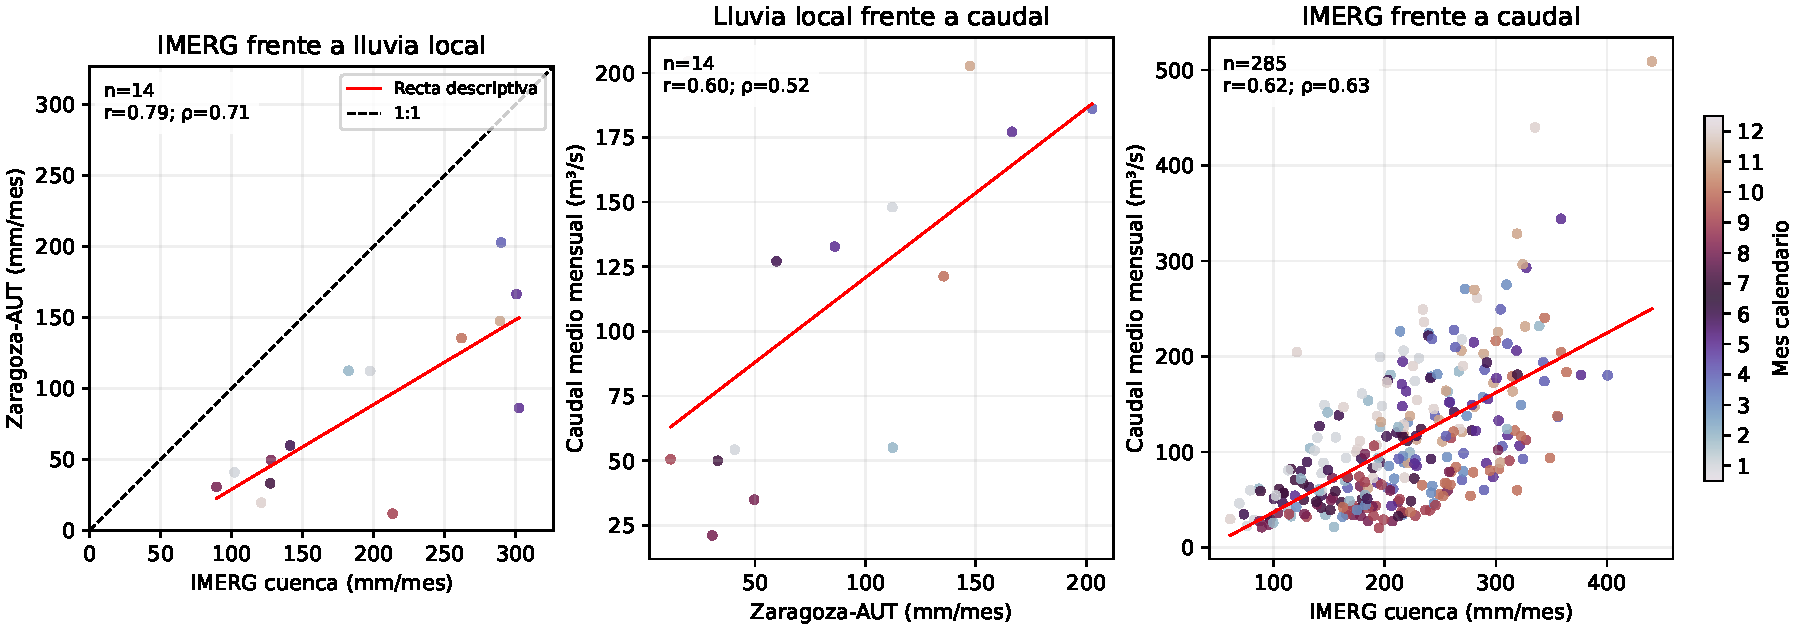
\includegraphics[width=\linewidth]{../apartado_2_1/dispersiones_21.pdf}\caption{Tres diagramas requeridos con IMERG de polígono y lluvia local completa.}\end{figure}
\subsubsection*{Los mismos diagramas para CHIRPS}\begin{figure}[H]\centering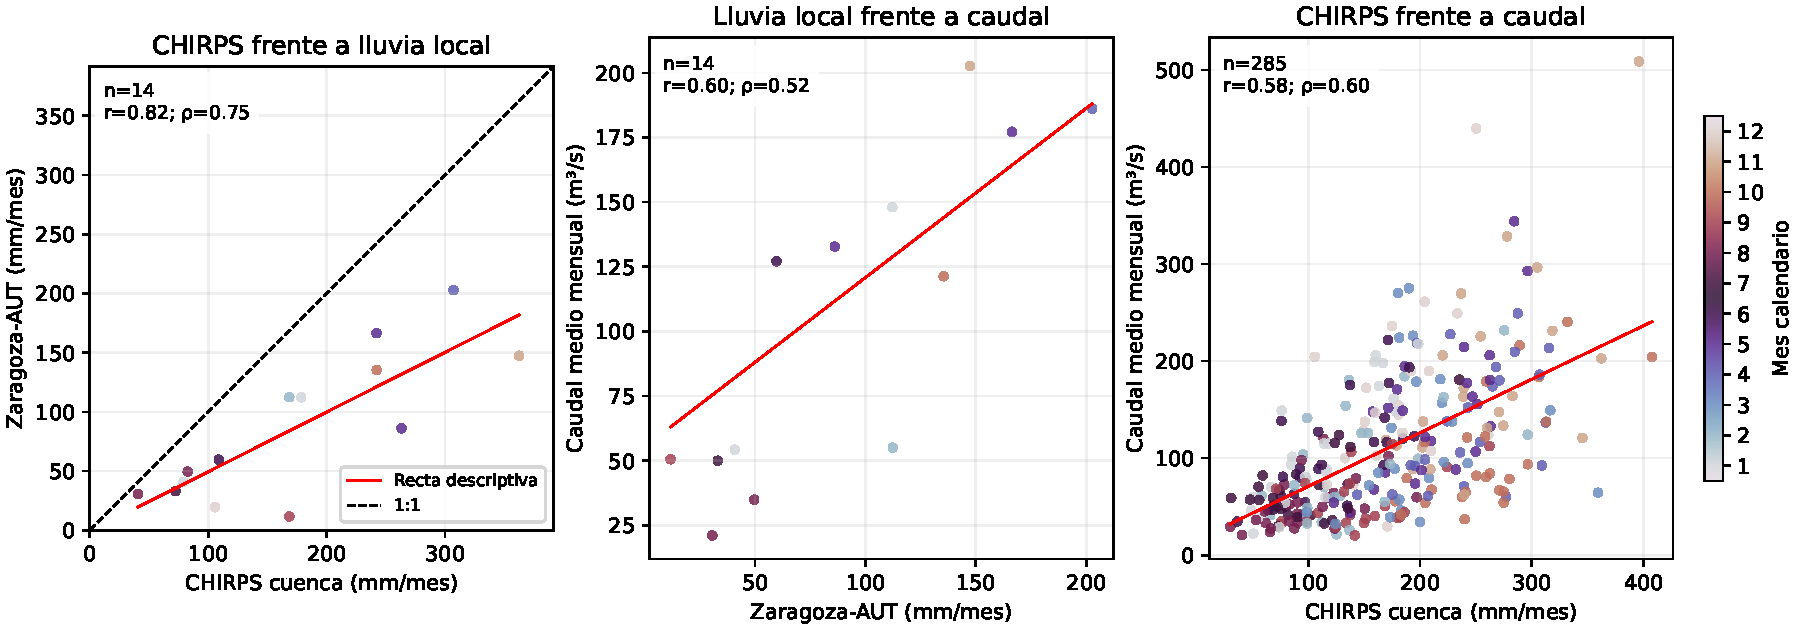
\includegraphics[width=\linewidth]{../apartado_2_1/dispersiones_CHIRPS_21.pdf}\caption{CHIRPS--lluvia local, lluvia local--Q y CHIRPS--Q; muestras comunes.}\end{figure}

\begin{figure}[H]\centering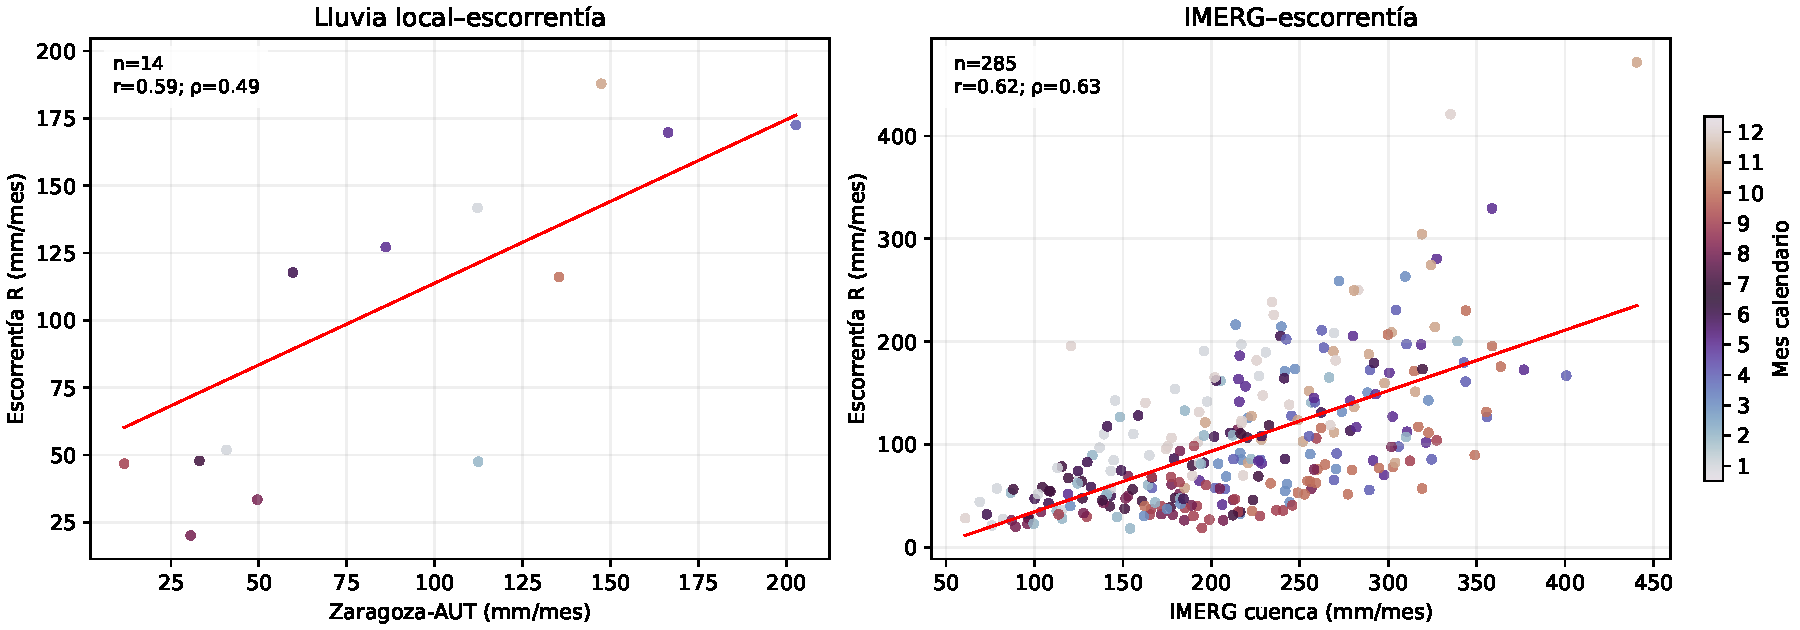
\includegraphics[width=\linewidth]{../apartado_2_1/laminas_21.pdf}\caption{Comparación de precipitación y escorrentía en láminas mensuales.}\end{figure}
\subsubsection*{Dirección, forma, dispersión y agrupamientos}
Las tres nubes muestran asociación positiva; IMERG--lluvia local es la más fuerte en la muestra pequeña, mientras lluvia local--Q e IMERG--Q son moderadas. La nube IMERG--Q es alargada y dispersa, sin una función única: una misma lluvia puede acompañarse de caudales diferentes. Los meses calendario se solapan; el color ayuda a detectar agrupamientos estacionales, pero no establece regímenes separados. No hay soporte para ajustar curvaturas con solo 14 puntos locales. Se observan puntos de Q alto fuera del núcleo de la nube; una mayor amplitud a magnitudes altas puede sugerir variabilidad dependiente de la magnitud, pero no constituye una prueba de heterocedasticidad.
\subsubsection*{Sesgo, MAE y RMSE frente a la referencia local}
La línea 1:1 usa límites y escalas iguales. Con lluvia local como referencia, el error mensual se define mediante
\begin{equation}
e_t=P_{\mathrm{IMERG},t}-L_t
\end{equation}
El sesgo medio es +109,80 mm/mes, MAE 109,80 mm/mes y RMSE 119,61 mm/mes (n=14). El sesgo indica la diferencia media con signo; MAE mide la diferencia absoluta típica; RMSE da más peso a errores grandes. Todos los errores de esta muestra son positivos, por eso sesgo y MAE coinciden. IMERG es un promedio de cuenca y Zaragoza una medición puntual: la diferencia combina representatividad espacial, cobertura y errores de ambas fuentes; no es una validación contra la lluvia verdadera de toda la cuenca. Una correlación alta no garantiza concordancia con 1:1.
\subsubsection*{Pearson, Spearman y valores influyentes}
Pearson resume asociación lineal y es sensible a magnitudes extremas; Spearman correlaciona rangos y resume asociación monótona. Sus diferencias no prueban por sí solas no linealidad. Se comprueba influencia retirando un mes cada vez: la tabla de sensibilidad muestra el mes que más cambia Pearson y el intervalo obtenido. No se eliminan extremos del análisis. Noviembre y diciembre de 2010 destacan por caudales altos en IMERG--Q; diciembre de 2018 combina poca lluvia local y caudal alto, compatible con lluvia antecedente o aportes de otras zonas. Son hipótesis de interpretación que requieren datos adicionales, no causas demostradas.
\begin{center}\small\begin{tabular}{lrrr}\hline
Relación & n & Pearson & Spearman \\ \hline
IMERG--lluvia local & 14 & 0,79 & 0,71 \\
Lluvia local--caudal & 14 & 0,60 & 0,52 \\
IMERG--caudal & 285 & 0,62 & 0,63 \\
IMERG--escorrentía & 285 & 0,62 & 0,63 \\
\hline\end{tabular}\end{center}
\begin{center}\small\begin{tabular}{lrrrr}\hline
Relación & Mes influyente & r sin mes & r mínimo & r máximo \\ \hline
IMERG--lluvia local & 2018-09 & 0,87 & 0,75 & 0,87 \\
Lluvia local--caudal & 2018-12 & 0,84 & 0,53 & 0,84 \\
IMERG--caudal & 2010-11 & 0,60 & 0,60 & 0,63 \\
IMERG--escorrentía & 2010-11 & 0,60 & 0,60 & 0,63 \\
\hline\end{tabular}\end{center}
\subsubsection*{Rezagos mensuales y apoyo con láminas}
Se relaciona la lluvia antecedente con el caudal mediante
\begin{equation}
\rho(k)=\operatorname{corr}\!\left[P(t-k),Q(t)\right],\qquad k\geq 0
\end{equation}
Un rezago de un mes significa que se utiliza la lluvia del mes anterior. Se preserva el calendario mensual antes de desplazar, para no saltar faltantes. Se exploran 0--3 meses por posible humedad antecedente y almacenamiento; no se invocan nieve ni regulación documentada para explicar esta cuenca. Nunca se usa lluvia futura para explicar caudal pasado. Las muestras cambian por disponibilidad: los máximos de correlación son descriptivos y no estiman automáticamente un tiempo físico de respuesta. La comparación en láminas usa la conversión a escorrentía mensual
\begin{equation}
R_m=\frac{86{,}4\,d_m\,Q_m}{2797{,}19}\quad[\mathrm{mm/mes}]
\end{equation}
Aquí, $d_m$ es el número de días del mes y $Q_m$ el caudal medio mensual en m$^3$/s. R deriva de Q y no aporta evidencia independiente; sus diferencias mensuales incluyen la duración del mes. Los diagramas P--R ayudan a comparar unidades, pero no cierran un balance hídrico sin evapotranspiración y almacenamiento. En IMERG--Q, Pearson original es mayor sin rezago (0,62), mientras Spearman es ligeramente mayor a un mes (0,65 frente a 0,63): no hay un único rezago óptimo independiente del indicador. Con anomalías, el mayor valor de ambas correlaciones ocurre sin rezago (Pearson 0,64; Spearman 0,60). Para lluvia local--Q el máximo explorado es un mes (Pearson 0,65; Spearman 0,64), pero solo hay 14 pares y las muestras cambian. La correlación negativa a tres meses puede mezclar estacionalidad y tamaño muestral; no demuestra una respuesta física inversa.
\textbf{Rezagos: original.} $P(t-k)$ frente a $Q(t)$ o $R(t)$.
\begin{center}\small\begin{tabular}{lrrrr}\hline
Relación & k & n & Pearson & Spearman \\ \hline
Lluvia local--caudal & 0 & 14 & 0,60 & 0,52 \\
Lluvia local--caudal & 1 & 14 & 0,65 & 0,64 \\
Lluvia local--caudal & 2 & 14 & 0,14 & 0,09 \\
Lluvia local--caudal & 3 & 14 & -0,43 & -0,43 \\
IMERG--caudal & 0 & 285 & 0,62 & 0,63 \\
IMERG--caudal & 1 & 284 & 0,60 & 0,65 \\
IMERG--caudal & 2 & 283 & 0,32 & 0,36 \\
IMERG--caudal & 3 & 282 & 0,08 & 0,06 \\
IMERG--escorrentía & 0 & 285 & 0,62 & 0,63 \\
IMERG--escorrentía & 1 & 284 & 0,60 & 0,66 \\
IMERG--escorrentía & 2 & 283 & 0,32 & 0,36 \\
IMERG--escorrentía & 3 & 282 & 0,07 & 0,06 \\
\hline\end{tabular}\end{center}
\textbf{Rezagos: anomalia.} $P(t-k)$ frente a $Q(t)$ o $R(t)$.
\begin{center}\small\begin{tabular}{lrrrr}\hline
Relación & k & n & Pearson & Spearman \\ \hline
IMERG--caudal & 0 & 285 & 0,64 & 0,60 \\
IMERG--caudal & 1 & 284 & 0,50 & 0,50 \\
IMERG--caudal & 2 & 283 & 0,41 & 0,44 \\
IMERG--caudal & 3 & 282 & 0,43 & 0,46 \\
IMERG--escorrentía & 0 & 285 & 0,63 & 0,60 \\
IMERG--escorrentía & 1 & 284 & 0,50 & 0,50 \\
IMERG--escorrentía & 2 & 283 & 0,41 & 0,44 \\
IMERG--escorrentía & 3 & 282 & 0,42 & 0,45 \\
\hline\end{tabular}\end{center}
\subsubsection*{Anomalías y persistencia al retirar el ciclo anual}
La anomalía mensual se define como
\begin{equation}
X'(t)=X(t)-\overline{X}_{j(t)}
\end{equation}
La media de referencia corresponde al mes calendario $j(t)$. Para I, Q y R se calcula una climatología común de enero de 1998--diciembre de 2022 usando exclusivamente los 285 meses simultáneos completos; el archivo de climatología conserva el conteo por mes. La misma definición deberá utilizarse al integrar los apartados 1.5 y 3.2. La asociación IMERG--Q persiste después de retirar el ciclo anual: se reportan Pearson y Spearman de las anomalías y sus rezagos. Esto indica asociación entre desviaciones respecto de lo habitual, sin demostrar causalidad ni capacidad predictiva. No se presenta una climatología local como confiable: Zaragoza tiene solo 14 meses válidos, marzo no tiene ninguno y varios meses tienen un solo año. No es defendible completar la comparación de anomalías de las dos parejas locales con esa cobertura; se necesitan más años de lluvia local verificada. Sin rezago, las anomalías IMERG--Q dan Pearson 0,64 y Spearman 0,60.
\begin{figure}[H]\centering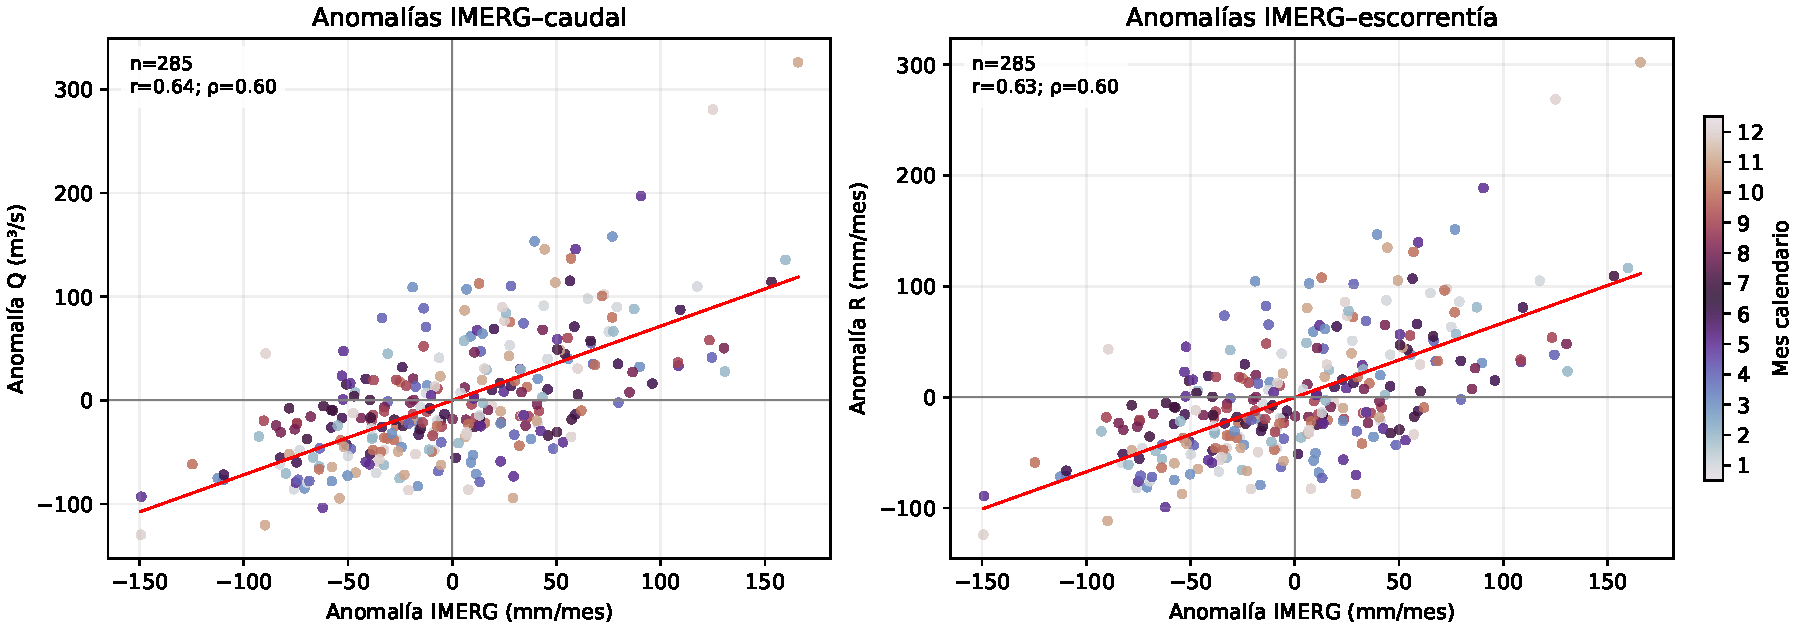
\includegraphics[width=\linewidth]{../apartado_2_1/anomalias_21.pdf}\caption{Anomalías con climatología común 1998--2022.}\end{figure}
\subsubsection*{CHIRPS e IMERG: comparación del apartado 2.1}
\subsubsection*{CHIRPS: los mismos diagramas y criterios}
Los diagramas comparan CHIRPS con la lluvia local y el caudal, bajo las mismas unidades y colores por mes calendario que IMERG. Ambos productos representan precipitación promediada sobre la cuenca. Se utilizan las mismas fechas para cada contraste: 14 meses completos frente a Zaragoza y 285 frente a caudal y escorrentía durante 1998--2022. Esto permite comparar los productos sin confundir sus diferencias con cambios en la cobertura temporal.

\subsubsection*{Dirección, forma, dispersión y puntos influyentes en CHIRPS}
CHIRPS--lluvia local y CHIRPS--Q muestran asociación positiva. La primera nube es relativamente alineada en esta muestra pequeña, aunque todos los acumulados CHIRPS están por encima de la lluvia local (debajo de 1:1 con la orientación elegida). CHIRPS--Q tiene una nube amplia; a lluvias similares corresponden caudales diferentes y no hay una relación determinista. Los colores se solapan, sin agrupamientos separados que permitan identificar regímenes por sí solos. En ambas fuentes, los caudales altos amplían la dispersión y noviembre de 2010 debe examinarse como valor influyente. La tabla de retirar-un-mes cuantifica la sensibilidad para cada relación; se conservan todos los valores originales.
\subsubsection*{¿Cuál tiene menor error frente a Zaragoza?}
En los mismos 14 meses, CHIRPS tiene sesgo +86,74, MAE 86,74 y RMSE 104,14 mm/mes; IMERG tiene sesgo +109,80, MAE 109,80 y RMSE 119,61 mm/mes. CHIRPS muestra menor discrepancia con la referencia puntual en esta muestra: su RMSE es aproximadamente 12,9 \% menor y su MAE 21,0 \% menor. Ambos sobreestiman todos los acumulados locales seleccionados. La relación CHIRPS--local es algo más fuerte (Pearson 0,82; Spearman 0,75) que IMERG--local (0,79; 0,71), pero la correlación no mide concordancia ni demuestra mayor exactitud en toda la cuenca. Zaragoza es una referencia puntual de cobertura corta; no basta para declarar un producto superior en general.
\begin{center}\small\begin{tabular}{lrrrrr}\hline
Fuente & n & Sesgo & MAE & RMSE & SD error \\ \hline
IMERG & 14 & 109,80 & 109,80 & 119,61 & 49,22 \\
CHIRPS & 14 & 86,74 & 86,74 & 104,14 & 59,80 \\
\hline\end{tabular}\end{center}
\subsubsection*{¿Cuál es más disperso? Depende de la comparación}
La dispersión se cuantifica con unidades y muestras iguales. Frente a la recta 1:1 con Zaragoza, la desviación estándar muestral del error P-local es 59,80 mm/mes para CHIRPS y 49,22 para IMERG: los errores CHIRPS son más variables aunque su sesgo y RMSE totales son menores. Alrededor de la recta lineal ajustada a lluvia local, el RMSE residual es 33,59 mm/mes para CHIRPS y 35,87 para IMERG: la nube CHIRPS es algo más estrecha alrededor de su propia recta. Frente a caudal, el RMSE residual en los mismos 285 meses es 58,89 m$^3$/s para CHIRPS y 56,85 para IMERG: IMERG tiene aproximadamente 3,5 \% menos dispersión residual y una asociación algo mayor. Estas rectas son resúmenes descriptivos calculados con todos los pares, no modelos validados ni errores de pronóstico.
\begin{center}\small\begin{tabular}{lrrrr}\hline
Fuente & Referencia & n & RMSE residual & Mediana abs. \\ \hline
IMERG & lluvia local & 14 & 35,87 & 14,86 \\
IMERG & caudal Q & 285 & 56,85 & 35,49 \\
IMERG & escorrentía R & 285 & 53,58 & 32,64 \\
CHIRPS & lluvia local & 14 & 33,59 & 25,80 \\
CHIRPS & caudal Q & 285 & 58,89 & 33,70 \\
CHIRPS & escorrentía R & 285 & 55,60 & 31,76 \\
\hline\end{tabular}\end{center}
\subsubsection*{Anomalías, rezagos y apoyo con escorrentía para CHIRPS}
Se resta la climatología de cada mes calendario construida con los mismos 285 meses de 1998--2022 para CHIRPS, IMERG, Q y R. CHIRPS--Q pasa de Pearson 0,58 y Spearman 0,60 en valores originales a 0,54 y 0,54 en anomalías. IMERG--Q pasa de 0,62 y 0,63 a 0,64 y 0,60. La asociación persiste para ambas fuentes; IMERG es más fuerte en anomalías dentro de este periodo común. Se exploran P(t-k) frente a Q(t)/R(t), con k=0--3 meses, preservando el calendario y excluyendo cada par inválido. La tabla permite contrastar los rezagos sin introducir lluvia futura. R se expresa en mm/mes y deriva de Q, por lo que no constituye evidencia independiente. Para las dos parejas con lluvia local permanece la limitación: los 14 meses no sustentan una climatología local de doce meses adecuada. Para CHIRPS, en original, el mayor Pearson explorado está en k=1 (0,60; n=274). No es una estimación causal del tiempo de respuesta. Para IMERG, en original, el mayor Pearson explorado está en k=0 (0,62; n=285). No es una estimación causal del tiempo de respuesta. Para CHIRPS, en anomalía, el mayor Pearson explorado está en k=0 (0,54; n=285). No es una estimación causal del tiempo de respuesta. Para IMERG, en anomalía, el mayor Pearson explorado está en k=0 (0,64; n=285). No es una estimación causal del tiempo de respuesta.
\begin{figure}[H]\centering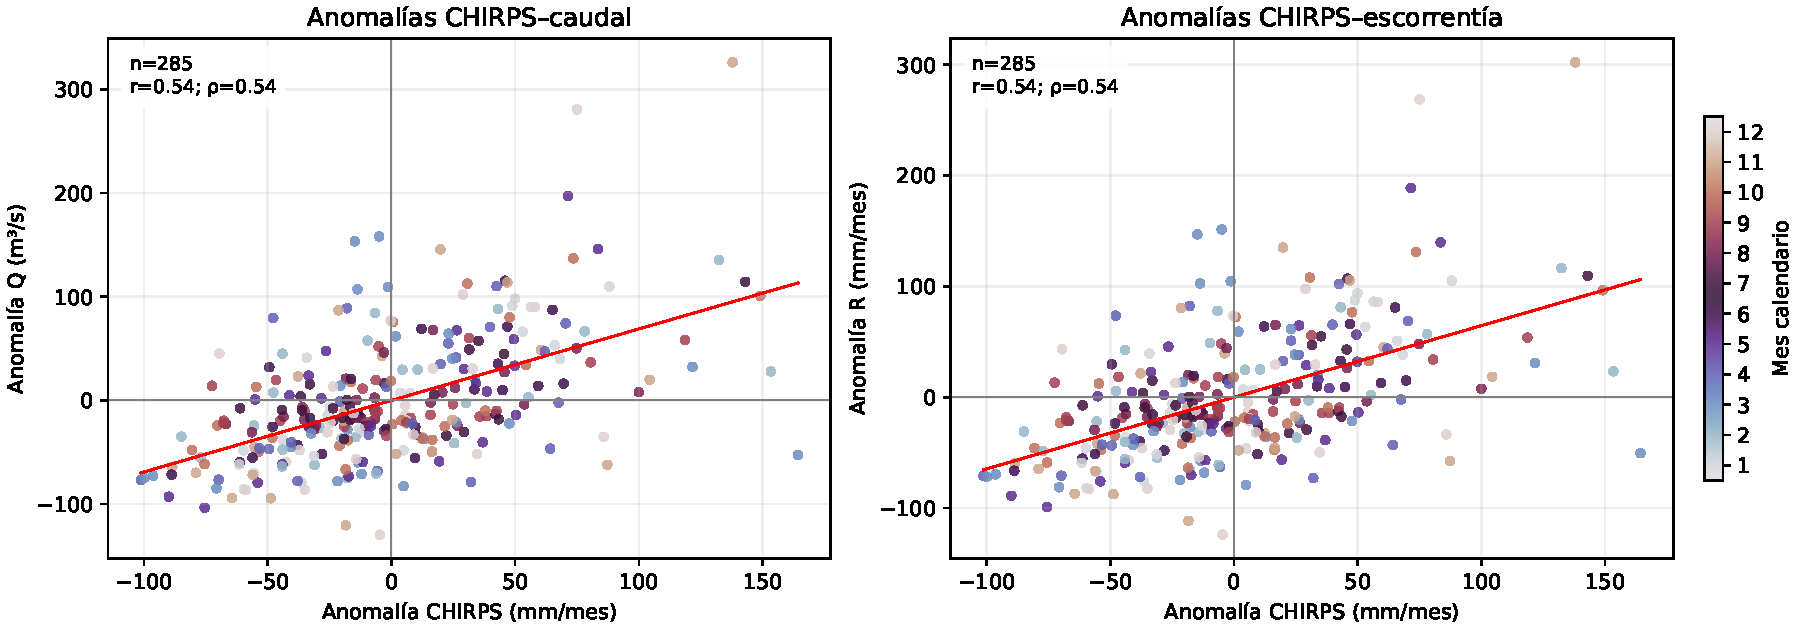
\includegraphics[width=\linewidth]{../apartado_2_1/anomalias_CHIRPS_21.pdf}\caption{Anomalías CHIRPS con climatología común 1998--2022.}\end{figure}
\begin{figure}[H]\centering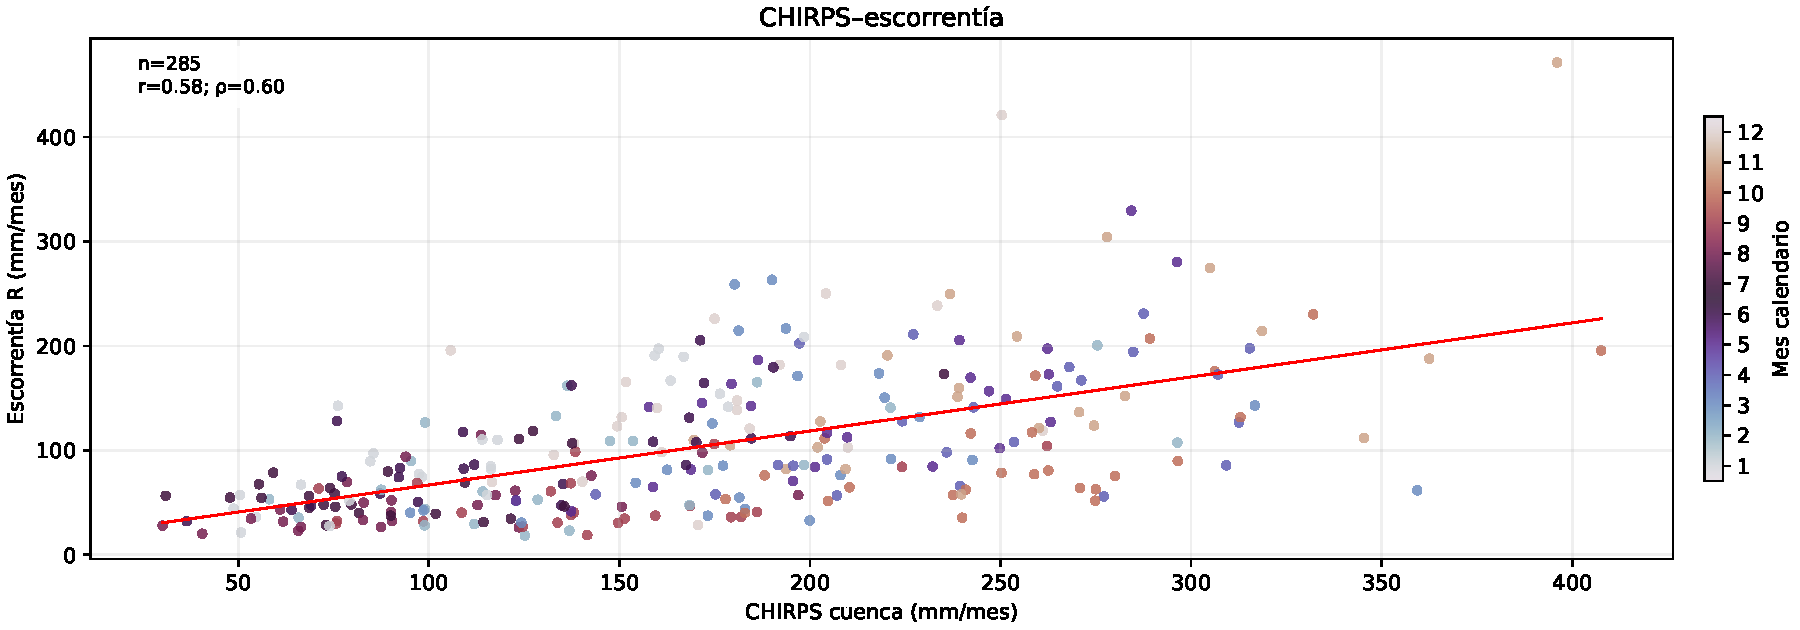
\includegraphics[width=\linewidth]{../apartado_2_1/laminas_CHIRPS_21.pdf}\caption{Apoyo con escorrentía mensual en láminas.}\end{figure}
\subsubsection*{Conclusión comparativa del 2.1}
CHIRPS se acerca más a Zaragoza en error medio y RMSE durante los 14 meses completos disponibles; IMERG se asocia algo más con el caudal y presenta menos dispersión alrededor de la recta P--Q en los 285 meses comunes, incluso después de retirar el ciclo anual. No hay un único ganador para todas las preguntas: error frente a lluvia local, variabilidad del error y asociación con caudal son criterios distintos. Ninguno de estos resultados demuestra causalidad ni una ventaja predictiva fuera de muestra. La comparación de anomalías locales requiere ampliar los registros completos de estaciones.
\subsubsection*{Correlaciones originales y anomalías: muestras comunes}
\begin{center}\small\begin{tabular}{lrrrrr}\hline
Fuente & Referencia & Serie & n & Pearson & Spearman \\ \hline
IMERG & lluvia local & original & 14 & 0,79 & 0,71 \\
IMERG & caudal Q & original & 285 & 0,62 & 0,63 \\
IMERG & caudal Q & anomalía & 285 & 0,64 & 0,60 \\
IMERG & escorrentía R & original & 285 & 0,62 & 0,63 \\
IMERG & escorrentía R & anomalía & 285 & 0,63 & 0,60 \\
CHIRPS & lluvia local & original & 14 & 0,82 & 0,75 \\
CHIRPS & caudal Q & original & 285 & 0,58 & 0,60 \\
CHIRPS & caudal Q & anomalía & 285 & 0,54 & 0,54 \\
CHIRPS & escorrentía R & original & 285 & 0,58 & 0,60 \\
CHIRPS & escorrentía R & anomalía & 285 & 0,54 & 0,54 \\
\hline\end{tabular}\end{center}
\subsubsection*{Sensibilidad CHIRPS: retirar un mes}
\begin{center}\small\begin{tabular}{lrrrr}\hline
Relación & Mes & r sin mes & r mínimo & r máximo \\ \hline
CHIRPS--lluvia local & 2018-09 & 0,87 & 0,78 & 0,87 \\
CHIRPS--caudal Q & 2010-11 & 0,56 & 0,56 & 0,59 \\
CHIRPS--escorrentía R & 2010-11 & 0,56 & 0,56 & 0,59 \\
\hline\end{tabular}\end{center}
\subsubsection*{Rezagos CHIRPS: calendario continuo}
\textbf{original.}\begin{center}\small\begin{tabular}{lrrrr}\hline
Referencia & k & n & Pearson & Spearman \\ \hline
caudal Q & 0,00 & 285 & 0,58 & 0,60 \\
caudal Q & 1,00 & 274 & 0,60 & 0,66 \\
caudal Q & 2,00 & 270 & 0,26 & 0,32 \\
caudal Q & 3,00 & 267 & -0,06 & -0,06 \\
escorrentía R & 0,00 & 285 & 0,58 & 0,60 \\
escorrentía R & 1,00 & 274 & 0,60 & 0,66 \\
escorrentía R & 2,00 & 270 & 0,27 & 0,32 \\
escorrentía R & 3,00 & 267 & -0,06 & -0,07 \\
\hline\end{tabular}\end{center}
\textbf{anomalía.}\begin{center}\small\begin{tabular}{lrrrr}\hline
Referencia & k & n & Pearson & Spearman \\ \hline
caudal Q & 0,00 & 285 & 0,54 & 0,54 \\
caudal Q & 1,00 & 274 & 0,41 & 0,42 \\
caudal Q & 2,00 & 270 & 0,30 & 0,36 \\
caudal Q & 3,00 & 267 & 0,30 & 0,35 \\
escorrentía R & 0,00 & 285 & 0,54 & 0,54 \\
escorrentía R & 1,00 & 274 & 0,41 & 0,42 \\
escorrentía R & 2,00 & 270 & 0,30 & 0,36 \\
escorrentía R & 3,00 & 267 & 0,30 & 0,35 \\
\hline\end{tabular}\end{center}

\subsection{Modelos estadísticos de lluvia y caudal}
Después de explorar las relaciones entre lluvia y caudal en los diagramas del apartado 2.1, buscamos establecer si esas asociaciones pueden traducirse en estimaciones útiles. Para ello construimos modelos estadísticos sencillos con dos propósitos: estimar la lluvia mensual de Zaragoza-AUT a partir de IMERG o CHIRPS, y estimar el caudal medio mensual del río La Vieja a partir de la precipitación de cuenca. También examinamos la relación entre lluvia local y caudal como un ejercicio exploratorio. El interés no está únicamente en encontrar una ecuación que se ajuste a los puntos, sino en comprobar si incorporar la lluvia mejora la estimación frente a referencias sencillas, como la media o el comportamiento habitual de cada mes.

En estos modelos, P(t) representa la precipitación de cuenca del mes t y L(t) la lluvia local, ambas en mm/mes; Q(t) corresponde al caudal medio mensual, expresado en m$^3$/s. IMERG se obtiene mediante un promedio por área sobre el polígono exacto de La Vieja. Comparamos las dos fuentes de precipitación en las mismas fechas para que las diferencias de desempeño respondan al modelo y al producto utilizado, y no a periodos distintos. Además de la lluvia del mes analizado, consideramos la del mes anterior como una forma sencilla de explorar la posible influencia de condiciones antecedentes sobre el caudal.

Esta comparación requiere que estén disponibles, simultáneamente, el caudal y la lluvia de IMERG y CHIRPS tanto en el mes actual como en el anterior. Al aplicar ese criterio, quedan 274 meses completos entre 1998 y 2022, once menos que los 285 pares contemporáneos del apartado 2.1; los faltantes se conservan sin rellenarlos. Organizamos esta muestra en el tiempo: los 206 meses disponibles hasta diciembre de 2016 se destinan al desarrollo y la selección de los modelos, mientras que los 68 meses de 2017--2022 se reservan para la evaluación del apartado 2.3. Así podemos elegir las ecuaciones con información del periodo de desarrollo y comprobar después cómo funcionan en meses que no intervinieron en esa elección.
\begin{samepage}\subsubsection*{Relaciones candidatas y criterio de selección}
La nube positiva de 2.1 justifica probar una recta como referencia, sin suponer que determine una respuesta única. Se comparan la media constante y la climatología mensual con cuatro relaciones que incorporan precipitación:
\begin{equation}
Q_t=a+bP_t
\end{equation}

\begin{equation}
Q_t=a+bP_{t-1}
\end{equation}

\begin{equation}
Q_t=a+bP_t+cP_{t-1}
\end{equation}

\begin{equation}
Q_t=a+b\sqrt{P_t}
\end{equation}
\end{samepage}
 La raíz cuadrada es una alternativa no lineal sencilla para una posible respuesta sublineal y no transforma el caudal. Se ajusta por mínimos cuadrados con intercepto, sin forzar paso por el origen. La selección usa RMSE agregado de tres validaciones temporales dentro del desarrollo: ajuste hasta 2006$\rightarrow$2007--2009, hasta 2009$\rightarrow$2010--2012 y hasta 2012$\rightarrow$2013--2016 (29, 30 y 46 meses, total 105). Cada coeficiente, media y climatología se estima solo con el pasado de su bloque. Se prefieren dos parámetros si el tercero mejora menos del 5 \%; se considera candidato útil si reduce al menos 5 \% el RMSE frente al mejor referente sin lluvia. Este umbral es una regla práctica explícita, no una prueba de significancia. La evaluación final independiente de 2017--2022 se realizará en 2.3.
\begin{center}\small\begin{tabular}{rrrrrrr}\hline
Fuente & Modelo & n & RMSE & MAE & Sesgo & $R^2$ \\ \hline
IMERG & Media constante & 105 & 83,17 & 60,06 & -2,25 & -0,04 \\
IMERG & Climatología mensual & 105 & 77,37 & 56,24 & -4,92 & 0,10 \\
IMERG & Lineal P(t) & 105 & 63,45 & 43,08 & -16,02 & 0,39 \\
IMERG & Lineal P(t-1) & 105 & 67,38 & 42,75 & -15,84 & 0,32 \\
IMERG & P(t) + P(t-1) & 105 & 56,43 & 38,97 & -22,66 & 0,52 \\
IMERG & Raíz de P(t) & 105 & 65,14 & 44,82 & -17,16 & 0,36 \\
CHIRPS & Media constante & 105 & 83,17 & 60,06 & -2,25 & -0,04 \\
CHIRPS & Climatología mensual & 105 & 77,37 & 56,24 & -4,92 & 0,10 \\
CHIRPS & Lineal P(t) & 105 & 69,42 & 48,58 & -2,19 & 0,27 \\
CHIRPS & Lineal P(t-1) & 105 & 71,36 & 50,57 & -3,21 & 0,23 \\
CHIRPS & P(t) + P(t-1) & 105 & 63,87 & 45,99 & -2,81 & 0,38 \\
CHIRPS & Raíz de P(t) & 105 & 70,19 & 49,80 & -3,91 & 0,26 \\
\hline\end{tabular}\end{center}
\subsubsection*{Resultado para caudal: modelos con lluvia actual y antecedente}
El modelo con P(t) y P(t-1) es el candidato seleccionado para ambas fuentes: mejora la recta contemporánea y los referentes de media y climatología. IMERG obtiene RMSE 56,43 m$^3$/s, MAE 38,97 y R$^2$ 0,52 en los 105 meses de validación de desarrollo; CHIRPS obtiene RMSE 63,87, MAE 45,99 y R$^2$ 0,38. La climatología tiene RMSE 77,37; la reducción es 27,1 \% para IMERG y 17,4 \% para CHIRPS. La raíz de P no supera al modelo con rezago. Esta evidencia respalda utilidad preliminar, no certifica predicción operativa. Las ecuaciones siguientes corresponden al reajuste final con los 206 meses de desarrollo; las métricas anteriores proceden de coeficientes ajustados por separado en cada bloque.

\begin{equation}
\widehat{Q}_t=\max\left(0,-87.2692+0.465439P_{IMERG,t}+0.433065P_{IMERG,t-1}\right).
\end{equation}


\begin{equation}
\widehat{Q}_t=\max\left(0,-35.8526+0.422155P_{CHIRPS,t}+0.434939P_{CHIRPS,t-1}\right).
\end{equation}

\begin{figure}[H]\centering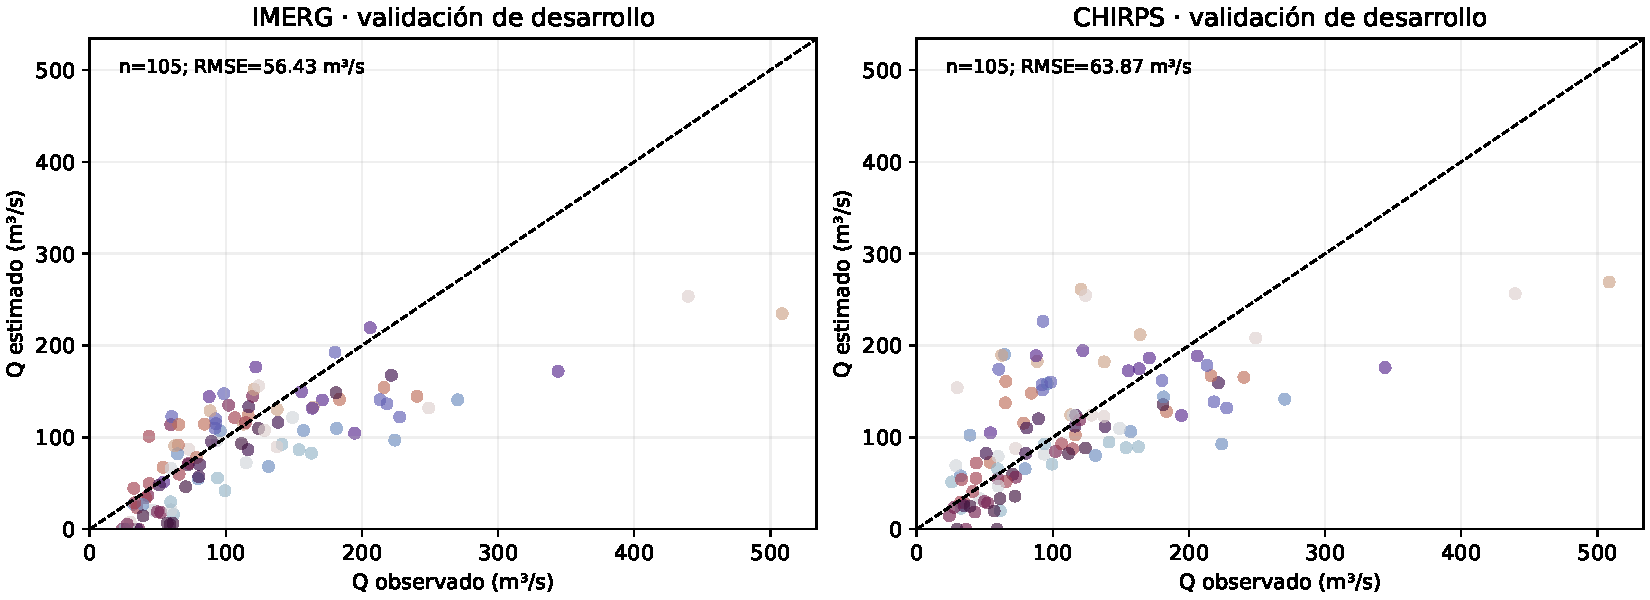
\includegraphics[width=\linewidth]{../apartado_2_2/modelos_Q_comparados.pdf}\caption{Modelos de caudal: validación temporal dentro del desarrollo.}\end{figure}
\begin{figure}[H]\centering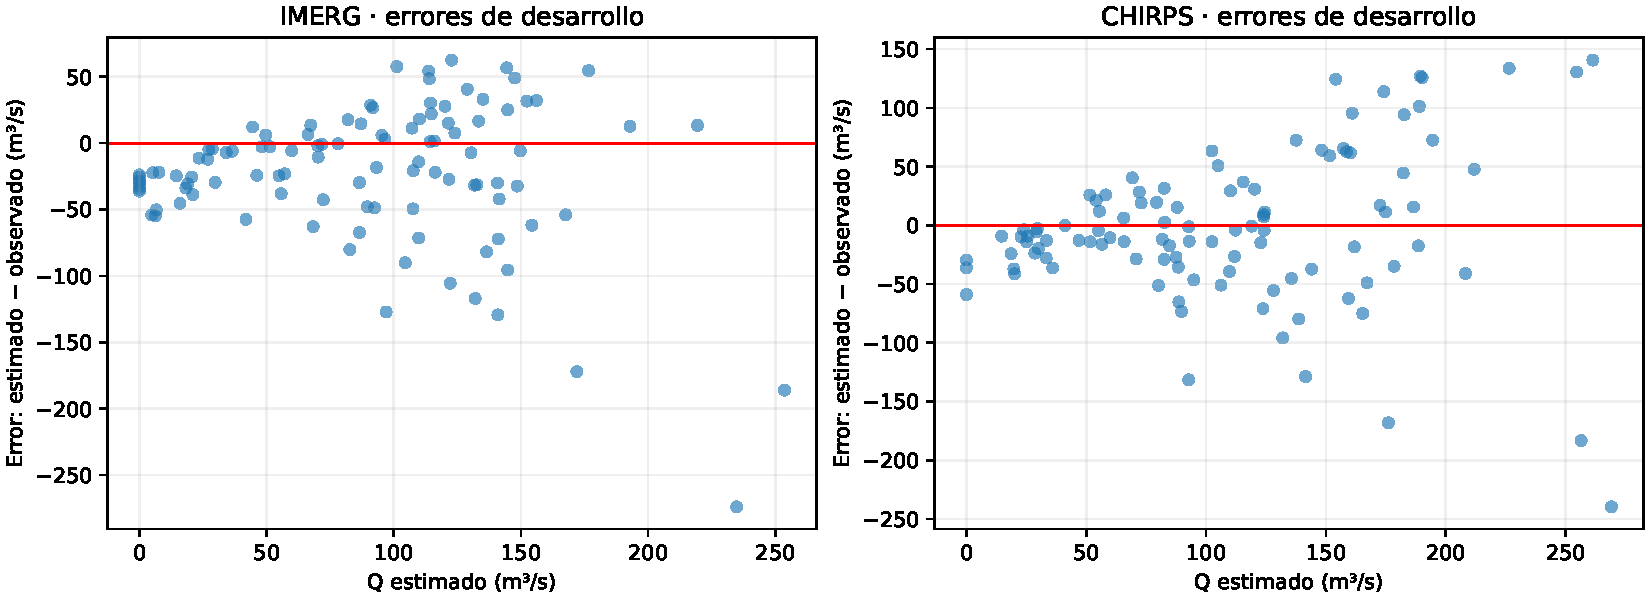
\includegraphics[width=\linewidth]{../apartado_2_2/residuos_Q.pdf}\caption{Errores de estimación de caudal durante la validación de desarrollo.}\end{figure}
\begin{center}\small\begin{tabular}{rrrrr}\hline
Fuente & Modelo & a & b & c \\ \hline
IMERG & Lineal P(t) & -26,10 & 0,61 & 0,00 \\
IMERG & Lineal P(t-1) & -22,11 & 0,60 & 0,00 \\
IMERG & P(t) + P(t-1) & -87,27 & 0,47 & 0,43 \\
IMERG & Raíz de P(t) & -138,95 & 16,97 & 0,00 \\
CHIRPS & Lineal P(t) & 10,97 & 0,57 & 0,00 \\
CHIRPS & Lineal P(t-1) & 9,20 & 0,59 & 0,00 \\
CHIRPS & P(t) + P(t-1) & -35,85 & 0,42 & 0,43 \\
CHIRPS & Raíz de P(t) & -70,49 & 14,11 & 0,00 \\
\hline\end{tabular}\end{center}
\subsubsection*{Lluvia local: calibración sencilla y evidencia limitada}
Se conserva solo la cobertura 100 \%: 14 meses completos. Para cada producto se comparan media, recta y raíz de P. La recta es la referencia elegida por parsimonia: la raíz no muestra una mejora convincente con tan pocos datos. En ajuste sobre los 14 meses, RMSE es 35,87 mm/mes para IMERG y 33,59 para CHIRPS. En un diagnóstico temporal muy corto (siete meses de 2018 para ajustar y siete de 2019 para comprobar), las rectas dan RMSE 41,85 para IMERG y 30,50 para CHIRPS; el referente constante da 58,03. Para IMERG, la raíz apenas mejora ese diagnóstico un 0,9 \%, insuficiente para preferirla; para CHIRPS empeora. No se selecciona por correlación ni se presenta el ajuste como validación. Estas ecuaciones calibran un promedio de cuenca hacia una estación puntual; no reconstruyen automáticamente la lluvia verdadera de toda la cuenca ni autorizan extrapolar a otras estaciones. Las ecuaciones mostradas usan los 14 meses, mientras la comprobación temporal usó únicamente coeficientes de 2018.

\begin{samepage}
\begin{equation}
\widehat{L}_t=\max\left(0,-30.7549+0.596818P_{IMERG,t}\right).
\end{equation}


\begin{equation}
\widehat{L}_t=\max\left(0,-0.9713+0.504221P_{CHIRPS,t}\right).
\end{equation}
\end{samepage}

\begin{center}\small\begin{tabular}{rrrrrr}\hline
Fuente & Modelo & RMSE ajuste & RMSE temporal & MAE temporal & $R^2$ temporal \\ \hline
IMERG & Media constante & 58,28 & 58,03 & 48,58 & -0,04 \\
IMERG & Lineal P(t) & 35,87 & 41,85 & 36,76 & 0,46 \\
IMERG & Raíz de P(t) & 36,25 & 41,47 & 36,76 & 0,47 \\
CHIRPS & Media constante & 58,28 & 58,03 & 48,58 & -0,04 \\
CHIRPS & Lineal P(t) & 33,59 & 30,50 & 25,58 & 0,71 \\
CHIRPS & Raíz de P(t) & 34,26 & 33,09 & 30,23 & 0,66 \\
\hline\end{tabular}\end{center}
\begin{figure}[H]\centering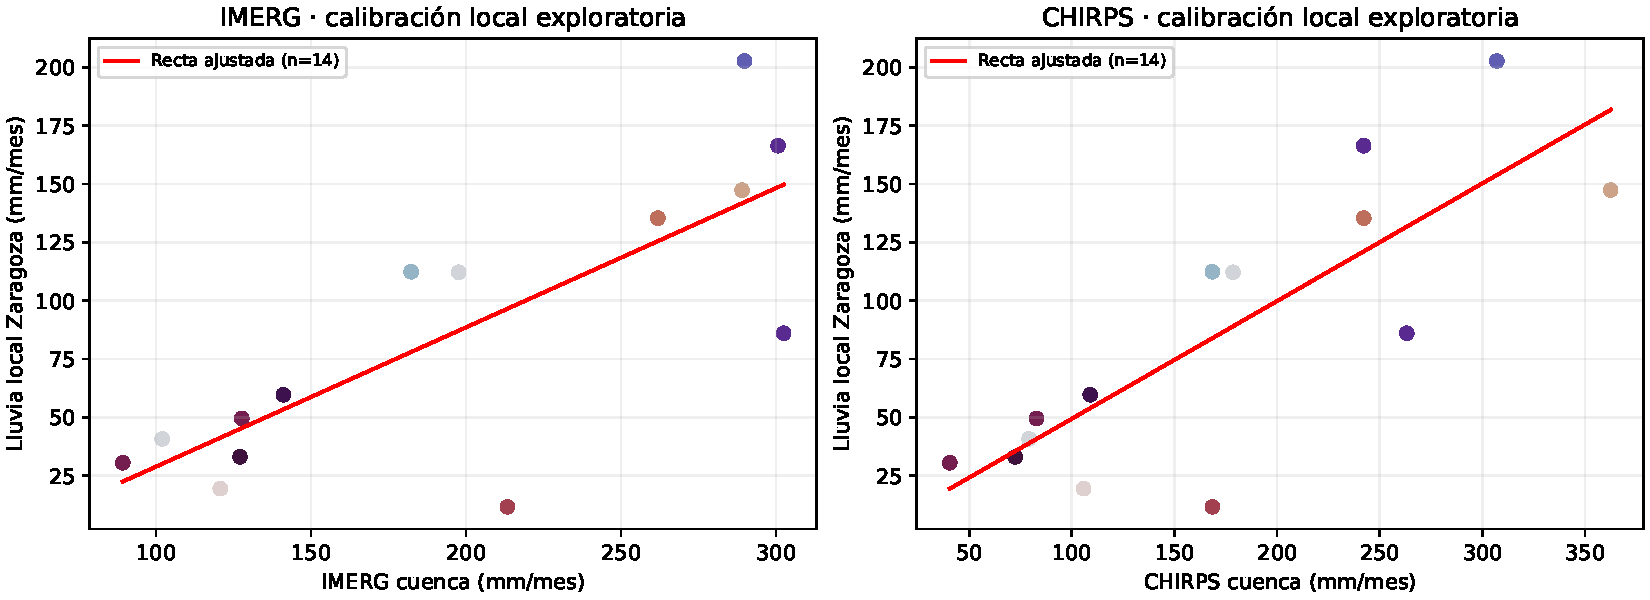
\includegraphics[width=\linewidth]{../apartado_2_2/modelos_lluvia_local.pdf}\caption{Calibraciones locales exploratorias, catorce meses de ajuste.}\end{figure}
\subsubsection*{Caudal a partir de lluvia local: no recomendar todavía}
La recta local--Q con 14 pares da RMSE de ajuste 51,13 m$^3$/s. En el diagnóstico temporal de siete meses de 2019, RMSE es 54,31 y R$^2$ solo 0,03, con sesgo +39,05 m$^3$/s; el referente constante tiene RMSE 71,01. La raíz empeora a RMSE 57,88 y R$^2$ negativo. Aunque la recta reduce error respecto de esa media, la explicación de la variabilidad es escasa, el sesgo es grande y el registro demasiado corto. Se documenta la ecuación exploratoria, pero no se recomienda un modelo operativo local--Q ni añadirle más parámetros o rezagos con esta muestra. No se compara directamente su RMSE de siete meses con los RMSE de 105 meses de IMERG/CHIRPS.

\begin{equation}
\widehat{Q}_t=\max\left(0,55.3322+0.654768L_t\right).
\end{equation}

\begin{center}\small\begin{tabular}{rrrrr}\hline
Modelo & RMSE ajuste & RMSE temporal & Sesgo temporal & $R^2$ temporal \\ \hline
media & 63,80 & 71,01 & 44,69 & -0,66 \\
lineal & 51,13 & 54,31 & 39,05 & 0,03 \\
raiz & 52,81 & 57,88 & 41,74 & -0,10 \\
\hline\end{tabular}\end{center}
\subsubsection*{Supuestos, rangos, ceros y transformaciones}
El modelo supone una relación aproximadamente estable en el periodo y ámbito de calibración; cambios de medición, uso del suelo, extracciones, humedad antecedente y regulación pueden romperla. Mínimos cuadrados minimiza errores cuadrados y es sensible a extremos. No se supone independencia de meses para calcular p-valores ni intervalos; los residuos pueden ser autocorrelacionados y de varianza cambiante. P(t-1) significa estrictamente el mes anterior del calendario, sin saltar faltantes. Las precipitaciones y caudales cero, si estuvieran observados, serían válidos; en las muestras actuales no hay ceros. La raíz admite cero y evita añadir constantes arbitrarias. Los faltantes nunca se sustituyen por cero. Para evitar estimaciones físicas negativas se publica max(0, expresión), también aplicado durante la comparación; no se recorta el extremo superior. No se recomienda extrapolar fuera de los rangos observados. Las ecuaciones con P(t) estiman el caudal una vez conocida la lluvia del mismo mes: no son pronósticos adelantados.
\begin{center}\small\begin{tabular}{rrrrr}\hline
Fuente & P mín. Q & P máx. Q & P mín. local & P máx. local \\ \hline
IMERG & 60,83 & 440,52 & 89,28 & 302,46 \\
CHIRPS & 30,12 & 396,03 & 40,56 & 362,47 \\
\hline\end{tabular}\end{center}
Rango de Q en desarrollo: 21,34--508,77 m$^3$/s.
\subsubsection*{Interpretación de parámetros y conservación de masa}
En lluvia local, el intercepto tiene unidades mm/mes y la pendiente es adimensional. En caudal, el intercepto está en m$^3$/s y las pendientes en (m$^3$/s)/(mm/mes); el coeficiente de $\sqrt{P}$ tendría unidades (m$^3$/s)/$\sqrt{\mathrm{mm/mes}}$. Una pendiente positiva indica asociación, no una fracción causal de lluvia convertida en caudal. El intercepto negativo y el truncamiento no representan un balance de agua. Q estimado puede convertirse a lámina mensual con la siguiente expresión:
\begin{equation}
\widehat{R}_m=\frac{86{,}4\,d_m\,\widehat{Q}_m}{2797{,}19}
\end{equation}
Sin embargo, la regresión no conserva masa: faltan evapotranspiración, cambios de almacenamiento, aportes, extracciones y controles de operación. No se interpreta P(t-1) como un tiempo de viaje medido.
\subsubsection*{Comparación y decisión del apartado 2.2}
Para lluvia local, la recta CHIRPS tiene mejor desempeño en el diagnóstico disponible, pero la muestra de 14 meses exige tratarla como calibración exploratoria. Para caudal, IMERG con lluvia actual y antecedente tiene menor RMSE y MAE de desarrollo que CHIRPS. Sin embargo, su sesgo es -22,66 m$^3$/s, frente a -2,81 de CHIRPS: menor error cuadrático no implica menor sesgo. Los gráficos de residuos permiten revisar magnitud y persistencia del error; no se prometen intervalos de predicción sin validación. Se proponen dos candidatos de caudal para pasar al 2.3, se mantienen calibraciones locales exploratorias y se descarta afirmar que la lluvia local corta sustenta un modelo operativo. En el cuartil de caudales observados más altos, ambos modelos subestiman y CHIRPS tiene menor RMSE (89,13 frente a 98,29 m$^3$/s de IMERG): la ventaja global de IMERG no se extiende automáticamente a extremos. La correlación de errores en meses consecutivos es 0,53 para IMERG y 0,67 para CHIRPS, señal de persistencia no resuelta. Esto limita la confianza en la relación y refuerza la necesidad del 2.3.
\begin{center}\small\begin{tabular}{rrrr}\hline
Fuente & r error antecedente & RMSE Q alto & Sesgo Q alto \\ \hline
IMERG & 0,53 & 98,29 & -76,29 \\
CHIRPS & 0,67 & 89,13 & -63,59 \\
\hline\end{tabular}\end{center}
\subsection{Desempeño de los modelos en la reserva temporal}
\subsubsection*{Partición temporal y prueba sin reajuste}
Se mantienen las decisiones del 2.2: modelos de caudal con lluvia del mismo mes y del mes anterior, ajustados con 206 meses válidos hasta diciembre de 2016. Aquí se abren únicamente los 68 meses comunes de enero de 2017 a diciembre de 2022. No se vuelven a elegir modelos, rezagos, transformaciones ni parámetros a partir de esta prueba. Los años completos definen la partición cronológica, pero se excluyen pares inválidos: junio y julio de 2021 y marzo y abril de 2022. Junio de 2021 y marzo de 2022 carecen de datos mensuales completos; los meses siguientes pierden la lluvia antecedente CHIRPS. No hay mezcla aleatoria de ajuste y prueba ni relleno de huecos. Se usa precipitación original, no anomalías, por lo que no se calcula una nueva climatología de predictores con la reserva.
\subsubsection*{Ecuaciones congeladas y referencia}
Se aplican exactamente las ecuaciones de caudal del 2.2, con el mismo truncamiento de los valores negativos:
\begin{equation}
\widehat{Q}_{\mathrm{IMERG},t}=\max\!\left(0,-87{,}269198+0{,}465439P_t+0{,}433065P_{t-1}\right)
\end{equation}

\begin{equation}
\widehat{Q}_{\mathrm{CHIRPS},t}=\max\!\left(0,-35{,}852625+0{,}422155P_t+0{,}434939P_{t-1}\right)
\end{equation}
 Q está en m$^3$/s y P en mm/mes. La referencia principal es la climatología mensual de Q estimada exclusivamente con los 206 meses de ajuste; también se muestra la media constante de ese ajuste. Se conserva una huella SHA-256 del archivo de parámetros para verificar que no cambió. Como P(t) se conoce al terminar el mes, esta prueba evalúa estimación mensual retrospectiva, no un pronóstico disponible antes de observar la lluvia del mes.
\subsubsection*{Resultados fuera del ajuste}
En los mismos 68 meses, CHIRPS obtiene RMSE 42,14 m$^3$/s, MAE 30,23, sesgo 2,47 y NSE 0,60; IMERG obtiene RMSE 43,77, MAE 34,49, sesgo -10,06 y NSE 0,57. El sesgo se define como estimado-observado: negativo indica subestimación. La eficiencia de Nash–Sutcliffe se calcula mediante
\begin{equation}
\mathrm{NSE}=1-\frac{\mathrm{SSE}}{\mathrm{SST}}
\end{equation}
Este indicador compara el error con la media del periodo evaluado; no sustituye la comparación explícita con la climatología entrenada. Esta última tiene RMSE 51,14. La reducción de RMSE frente a ella es 14,41 \% para IMERG y 17,61 \% para CHIRPS.
\begin{center}\small\begin{tabular}{lrrrrr}\hline
Fuente & n & RMSE & MAE & Sesgo & NSE \\ \hline
IMERG & 68 & 43,77 & 34,49 & -10,06 & 0,57 \\
CHIRPS & 68 & 42,14 & 30,23 & 2,47 & 0,60 \\
Media & 68 & 67,68 & 53,90 & -9,44 & -0,02 \\
Climatologia & 68 & 51,14 & 39,25 & -8,03 & 0,42 \\
\hline\end{tabular}\end{center}
\begin{figure}[H]\centering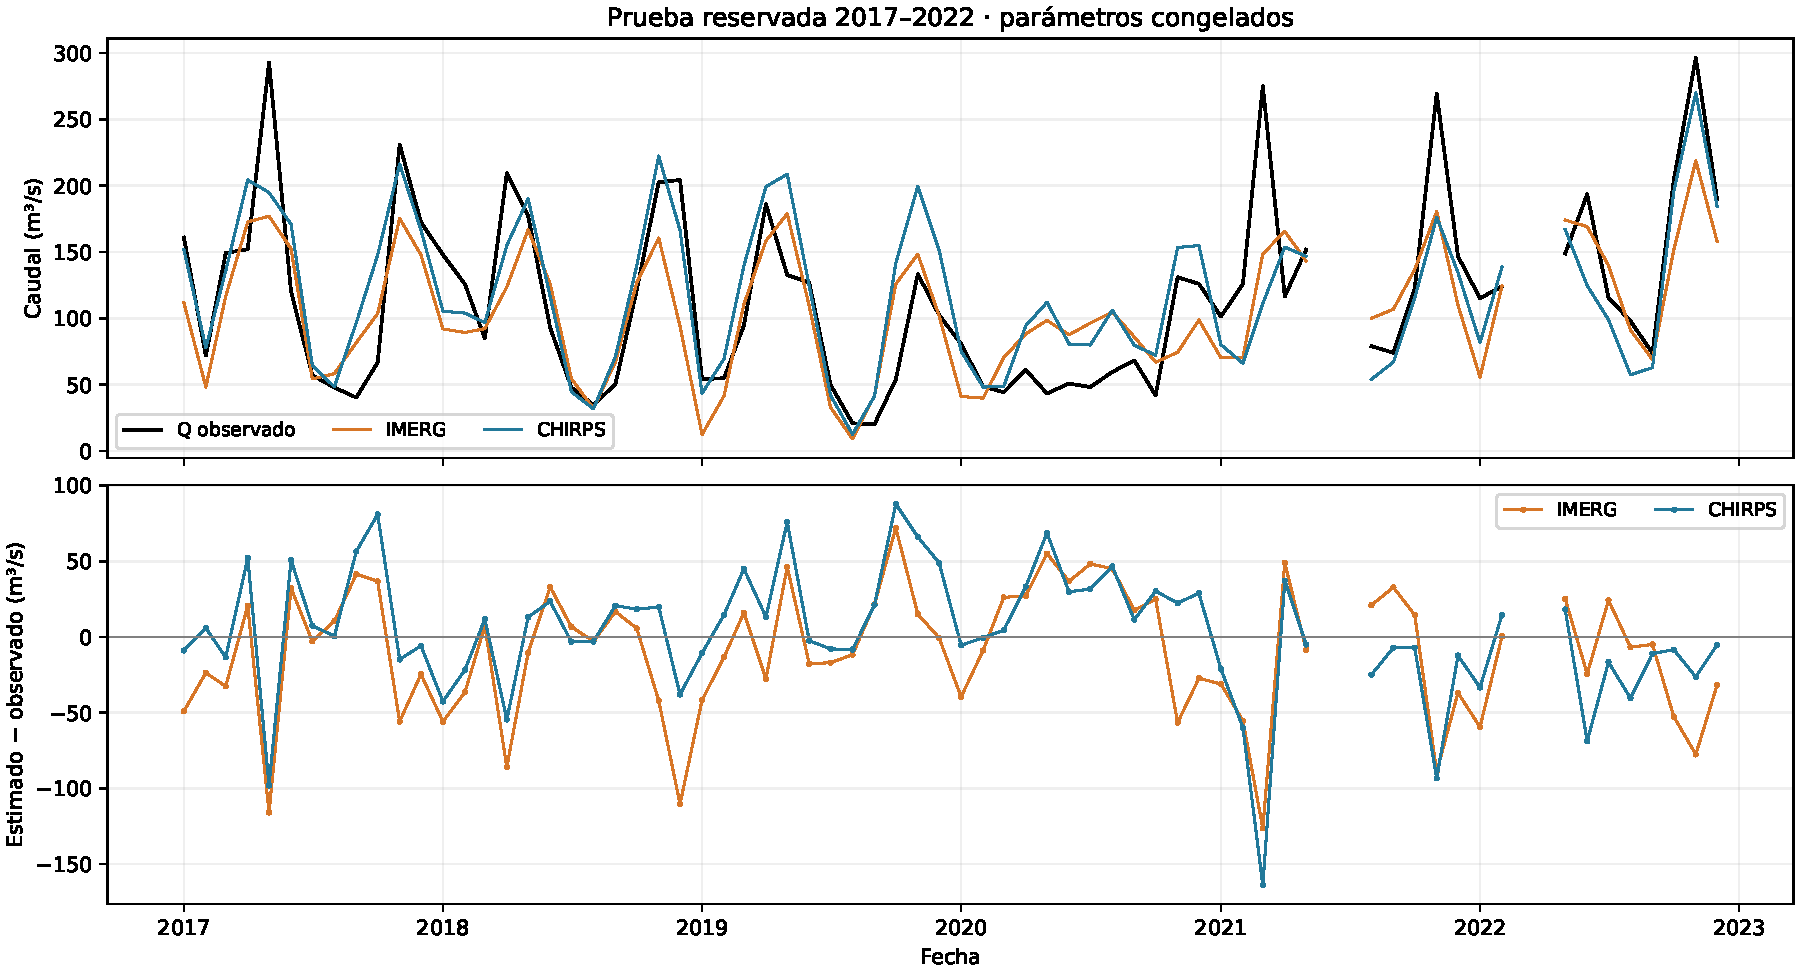
\includegraphics[width=\linewidth]{../apartado_2_3/reserva_series.pdf}\caption{Series y errores de los modelos congelados, 2017--2022.}\end{figure}
\subsubsection*{Estabilidad entre periodos y diferencia entre productos}
El orden de desempeño se invierte respecto del desarrollo: IMERG tenía RMSE 56,43 frente a 63,87 de CHIRPS; en la reserva CHIRPS es ligeramente mejor. La diferencia RMSE\_CHIRPS-RMSE\_IMERG es -1,63 m$^3$/s, pequeña frente al tamaño de los errores. La tabla anual permite examinar años favorables y desfavorables sin reajustar por año. Se calcula, además, un intervalo descriptivo de la diferencia mediante 3000 remuestreos pareados de bloques calendario de seis meses, manteniendo juntas las dos fuentes y preservando los huecos. Se repite con doce meses como sensibilidad; no se remuestrean meses aislados como si fueran independientes. Son intervalos aproximados con solo seis años, no una prueba de superioridad universal. El intervalo central del 95 \% con bloques de seis meses va de -7,76 a 5,89 m$^3$/s y con doce meses de -7,83 a 5,62; ambos incluyen cero. No hay evidencia sólida aquí de superioridad general de una fuente. CHIRPS tiene menor RMSE en 2017, 2018, 2020 y 2022; IMERG en 2019 y 2021. En 2020 el NSE es negativo para ambos (-0,59 y -0,17), lo que advierte estabilidad limitada respecto de la variabilidad de ese año, sin sustituir la referencia climatológica entrenada.
\begin{center}\small\begin{tabular}{lrrrrr}\hline
Fuente & Año & n & RMSE & MAE & Sesgo \\ \hline
IMERG & 2017 & 12 & 46,39 & 37,16 & -13,57 \\
IMERG & 2018 & 12 & 47,78 & 34,45 & -22,85 \\
IMERG & 2019 & 12 & 31,22 & 25,05 & 3,44 \\
IMERG & 2020 & 12 & 37,30 & 34,45 & 12,42 \\
IMERG & 2021 & 10 & 57,84 & 46,44 & -22,95 \\
IMERG & 2022 & 10 & 39,00 & 30,73 & -20,75 \\
CHIRPS & 2017 & 12 & 45,88 & 32,94 & 9,44 \\
CHIRPS & 2018 & 12 & 26,99 & 22,54 & -4,64 \\
CHIRPS & 2019 & 12 & 44,12 & 33,51 & 28,63 \\
CHIRPS & 2020 & 12 & 32,04 & 26,12 & 25,13 \\
CHIRPS & 2021 & 10 & 64,69 & 43,15 & -35,70 \\
CHIRPS & 2022 & 10 & 30,37 & 24,31 & -17,74 \\
Climatologia & 2017 & 12 & 52,57 & 36,85 & -22,10 \\
Climatologia & 2018 & 12 & 35,89 & 29,81 & -16,80 \\
Climatologia & 2019 & 12 & 38,79 & 36,16 & 22,30 \\
Climatologia & 2020 & 12 & 52,65 & 45,03 & 41,14 \\
Climatologia & 2021 & 10 & 60,98 & 38,53 & -33,12 \\
Climatologia & 2022 & 10 & 63,82 & 50,95 & -50,95 \\
\hline\end{tabular}\end{center}
\begin{center}\small\begin{tabular}{lrrr}\hline
Bloque (meses) & Diferencia RMSE & Percentil 2,5 & Percentil 97,5 \\ \hline
6 & -1,63 & -7,76 & 5,89 \\
12 & -1,63 & -7,83 & 5,62 \\
\hline\end{tabular}\end{center}
\subsubsection*{Residuos frente al tiempo, al estimado y al mes calendario}
Se presentan errores estimado-observado frente al tiempo y al valor estimado, además del sesgo y RMSE por mes calendario. Las curvas temporales conservan los huecos. La tabla mensual tiene solo cinco a seis observaciones por mes: las diferencias orientan la revisión, pero no justifican correcciones estacionales nuevas ajustadas con esta prueba. Se examina la correlación del error con el mes anterior usando el calendario completo, sin unir artificialmente meses separados por faltantes. Persistencia, dispersión cambiante y errores concentrados en ciertos meses limitan los modelos y evitan tratar una correlación global como garantía predictiva. IMERG subestima en enero, noviembre y diciembre (sesgos -46,14, -50,99 y -38,57 m$^3$/s); CHIRPS muestra sobreestimación marcada en octubre (+33,65) y subestimación en marzo (-23,16). Estos patrones no se corrigen después de mirar la reserva. La correlación del error con el mes anterior es 0,21 para IMERG y 0,18 para CHIRPS: la persistencia se reduce frente al desarrollo, pero no desaparece.
\begin{figure}[H]\centering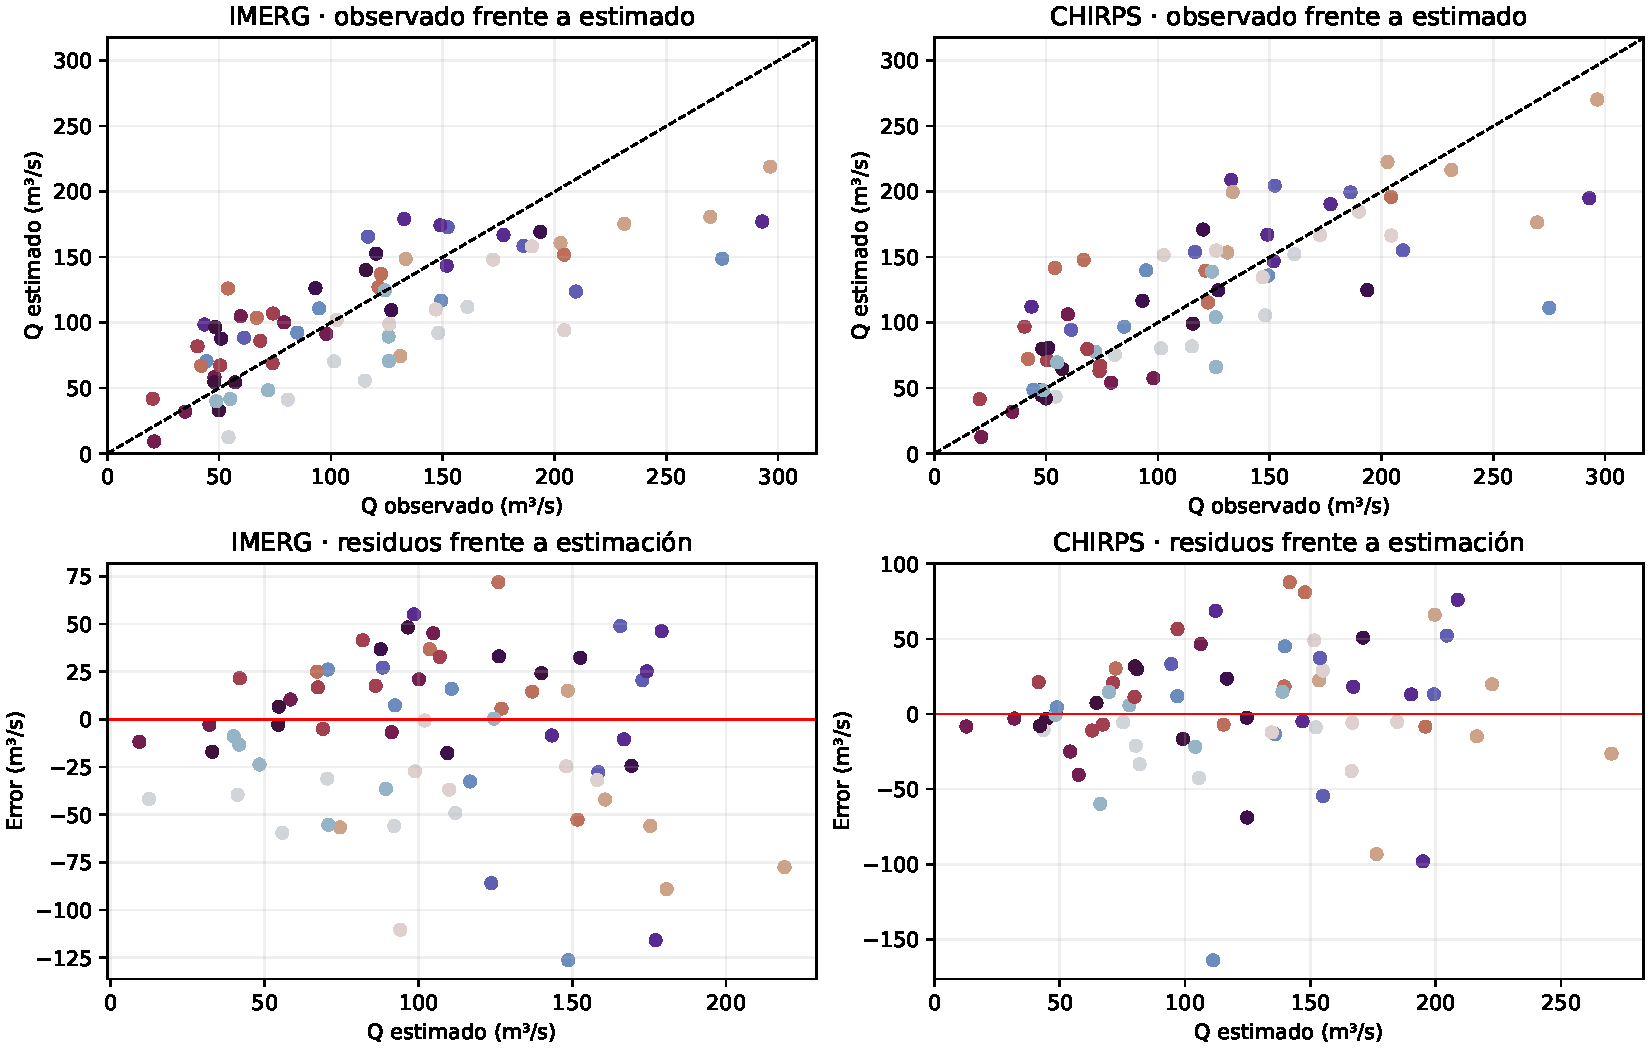
\includegraphics[width=\linewidth]{../apartado_2_3/reserva_dispersion_residuos.pdf}\caption{Predicciones y residuos frente al valor estimado.}\end{figure}
\begin{figure}[H]\centering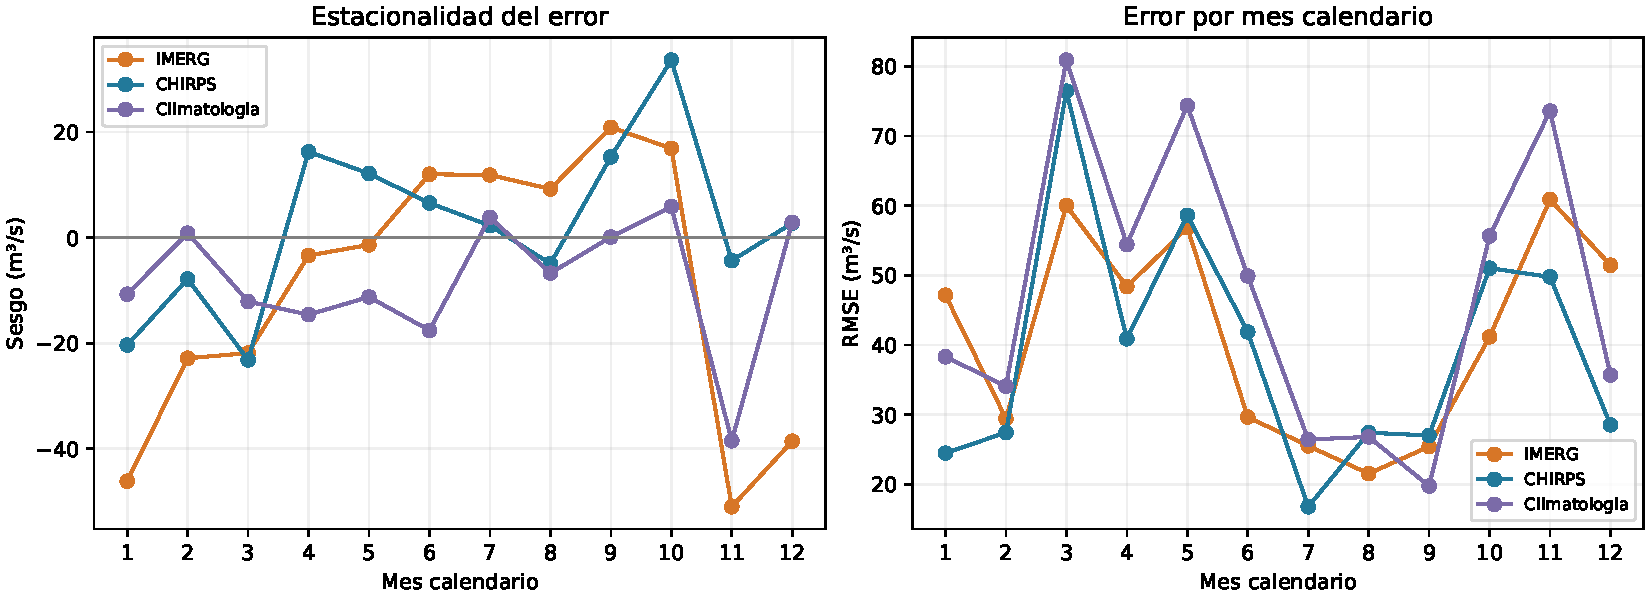
\includegraphics[width=\linewidth]{../apartado_2_3/reserva_meses.pdf}\caption{Estacionalidad residual y RMSE mensual en la reserva.}\end{figure}
\begin{center}\small\begin{tabular}{lrrrrr}\hline
Fuente & Mes & n & RMSE & MAE & Sesgo \\ \hline
IMERG & 1 & 6 & 47,16 & 46,14 & -46,14 \\
IMERG & 2 & 6 & 29,43 & 22,98 & -22,84 \\
IMERG & 3 & 5 & 60,02 & 41,69 & -21,86 \\
IMERG & 4 & 5 & 48,39 & 42,07 & -3,37 \\
IMERG & 5 & 6 & 56,86 & 43,52 & -1,37 \\
IMERG & 6 & 5 & 29,66 & 28,84 & 12,02 \\
IMERG & 7 & 5 & 25,52 & 19,79 & 11,88 \\
IMERG & 8 & 6 & 21,53 & 16,32 & 9,23 \\
IMERG & 9 & 6 & 25,43 & 22,54 & 20,89 \\
IMERG & 10 & 6 & 41,17 & 34,44 & 16,92 \\
IMERG & 11 & 6 & 60,89 & 56,01 & -50,99 \\
IMERG & 12 & 6 & 51,46 & 38,57 & -38,57 \\
CHIRPS & 1 & 6 & 24,47 & 20,35 & -20,35 \\
CHIRPS & 2 & 6 & 27,44 & 19,54 & -7,82 \\
CHIRPS & 3 & 5 & 76,44 & 47,75 & -23,16 \\
CHIRPS & 4 & 5 & 40,89 & 38,07 & 16,27 \\
CHIRPS & 5 & 6 & 58,62 & 46,46 & 12,15 \\
CHIRPS & 6 & 5 & 41,88 & 35,09 & 6,56 \\
CHIRPS & 7 & 5 & 16,77 & 13,35 & 2,29 \\
CHIRPS & 8 & 6 & 27,40 & 20,64 & -4,93 \\
CHIRPS & 9 & 6 & 27,02 & 21,32 & 15,31 \\
CHIRPS & 10 & 6 & 51,03 & 38,79 & 33,65 \\
CHIRPS & 11 & 6 & 49,78 & 40,45 & -4,35 \\
CHIRPS & 12 & 6 & 28,53 & 23,20 & 2,75 \\
\hline\end{tabular}\end{center}
\begin{center}\small\begin{tabular}{lrr}\hline
Fuente & r error antecedente & Fracción subestimada \\ \hline
IMERG & 0,21 & 0,56 \\
CHIRPS & 0,18 & 0,50 \\
\hline\end{tabular}\end{center}
\subsubsection*{Caudales altos, plausibilidad física y extrapolación}
Para definir caudal alto se usa el percentil 75 del ajuste, 141,54 m$^3$/s, sin elegir el umbral con la prueba. Se reportan por separado n, sesgo, MAE y RMSE de esa condición y del resto. En el grupo alto, el menor RMSE corresponde a CHIRPS (54,06 m$^3$/s), lo que debe leerse junto con los sesgos y la muestra. Se cuentan salidas negativas antes de aplicar el truncamiento a cero y entradas P(t) o P(t-1) fuera de los rangos del ajuste. El truncamiento asegura no negatividad, pero no conserva masa ni valida magnitudes extremas. No se aplica recorte superior, interpolación ni corrección posterior del sesgo. Cambios de almacenamiento, evapotranspiración, extracción y operación quedan fuera de estas regresiones. Los dos modelos subestiman caudales altos: sesgo -48,16 m$^3$/s para IMERG y -25,85 para CHIRPS, con 21 meses en el grupo. En los 47 meses bajos-medios, IMERG tiene menor RMSE (31,83 frente a 35,54). No hubo salidas brutas negativas en la reserva. CHIRPS presenta dos meses con predictores fuera del rango de ajuste, octubre y noviembre de 2022; IMERG ninguno. No se descartan esos meses para favorecer un resultado.
\textbf{Q alto (umbral de ajuste).}\begin{center}\small\begin{tabular}{lrrrr}\hline
Fuente & n & RMSE & MAE & Sesgo \\ \hline
IMERG & 21 & 62,74 & 52,52 & -48,16 \\
CHIRPS & 21 & 54,06 & 36,93 & -25,85 \\
Media & 21 & 102,94 & 91,20 & -91,20 \\
Climatologia & 21 & 73,94 & 59,13 & -57,89 \\
\hline\end{tabular}\end{center}
\textbf{Q bajo-medio.}\begin{center}\small\begin{tabular}{lrrrr}\hline
Fuente & n & RMSE & MAE & Sesgo \\ \hline
IMERG & 47 & 31,83 & 26,43 & 6,97 \\
CHIRPS & 47 & 35,54 & 27,24 & 15,13 \\
Media & 47 & 43,50 & 37,24 & 27,08 \\
Climatologia & 47 & 36,62 & 30,37 & 14,24 \\
\hline\end{tabular}\end{center}
\begin{center}\small\begin{tabular}{lrrrr}\hline
Fuente & Mín. bruto & Máx. bruto & Negativos & Fuera rango P \\ \hline
IMERG & 9,32 & 218,97 & 0 & 0 \\
CHIRPS & 12,76 & 270,15 & 0 & 2 \\
\hline\end{tabular}\end{center}
\subsubsection*{Comparación de estimaciones de lluvia local}
La tabla compara IMERG y CHIRPS sin corrección con sus rectas de calibración para estimar la lluvia mensual de Zaragoza. Las rectas se ajustaron con siete meses completos de 2018 y se comprobaron con siete de 2019; RMSE, MAE y sesgo se expresan en mm/mes. Por su corta duración y su uso en la selección de los modelos, esta comparación es exploratoria y no constituye una validación final independiente.
\begin{center}\small\begin{tabular}{lrrrrr}\hline
Fuente & Método & n & RMSE & MAE & Sesgo \\ \hline
IMERG & Sin corrección & 7 & 108,19 & 95,51 & 95,51 \\
IMERG & Recta de calibración & 7 & 41,85 & 36,76 & -17,40 \\
CHIRPS & Sin corrección & 7 & 85,28 & 67,75 & 67,75 \\
CHIRPS & Recta de calibración & 7 & 30,50 & 25,58 & -14,29 \\
\hline\end{tabular}\end{center}
\subsubsection*{Fuentes compartidas y alcance de la independencia}
La separación temporal evita usar el caudal de prueba para ajustar la regresión, pero no garantiza independencia entre productos de precipitación y estaciones. IMERG Final combina información satelital con análisis de pluviómetros; CHIRPS combina información satelital y estaciones. No se ha verificado si Zaragoza integra las redes de ajuste de estos productos. Tampoco se presenta Q como un balance de agua cerrado ni como una medida causal de la lluvia. Fuentes metodológicas: NASA, IMERG (\url{https://gpm.nasa.gov/data/imerg}); Climate Hazards Center, CHIRPS (\url{https://chc.ucsb.edu/data/chirps}). La reserva temporal permite evaluar la generalización del modelo; una comprobación prospectiva con años nuevos reforzaría la evidencia.
\subsubsection*{Conclusión del 2.3}
Existe una relación aprovechable para estimar caudal mensual a partir de lluvia contemporánea y antecedente: ambas fuentes mejoran la climatología en la prueba reservada. CHIRPS tiene el menor RMSE y MAE globales y un sesgo más cercano a cero en 2017--2022; la ventaja es pequeña y debe contrastarse con años, meses y condiciones de caudal, sin declarar un ganador general. Los modelos siguen siendo herramientas estadísticas retrospectivas de la misma cuenca, con limitaciones en extremos, estabilidad y causalidad. No se recomienda usarlos como pronósticos de crecidas ni extrapolarlos a otras cuencas.
\clearpage
% PUNTO_3_COMMIT_2D27402_INICIO
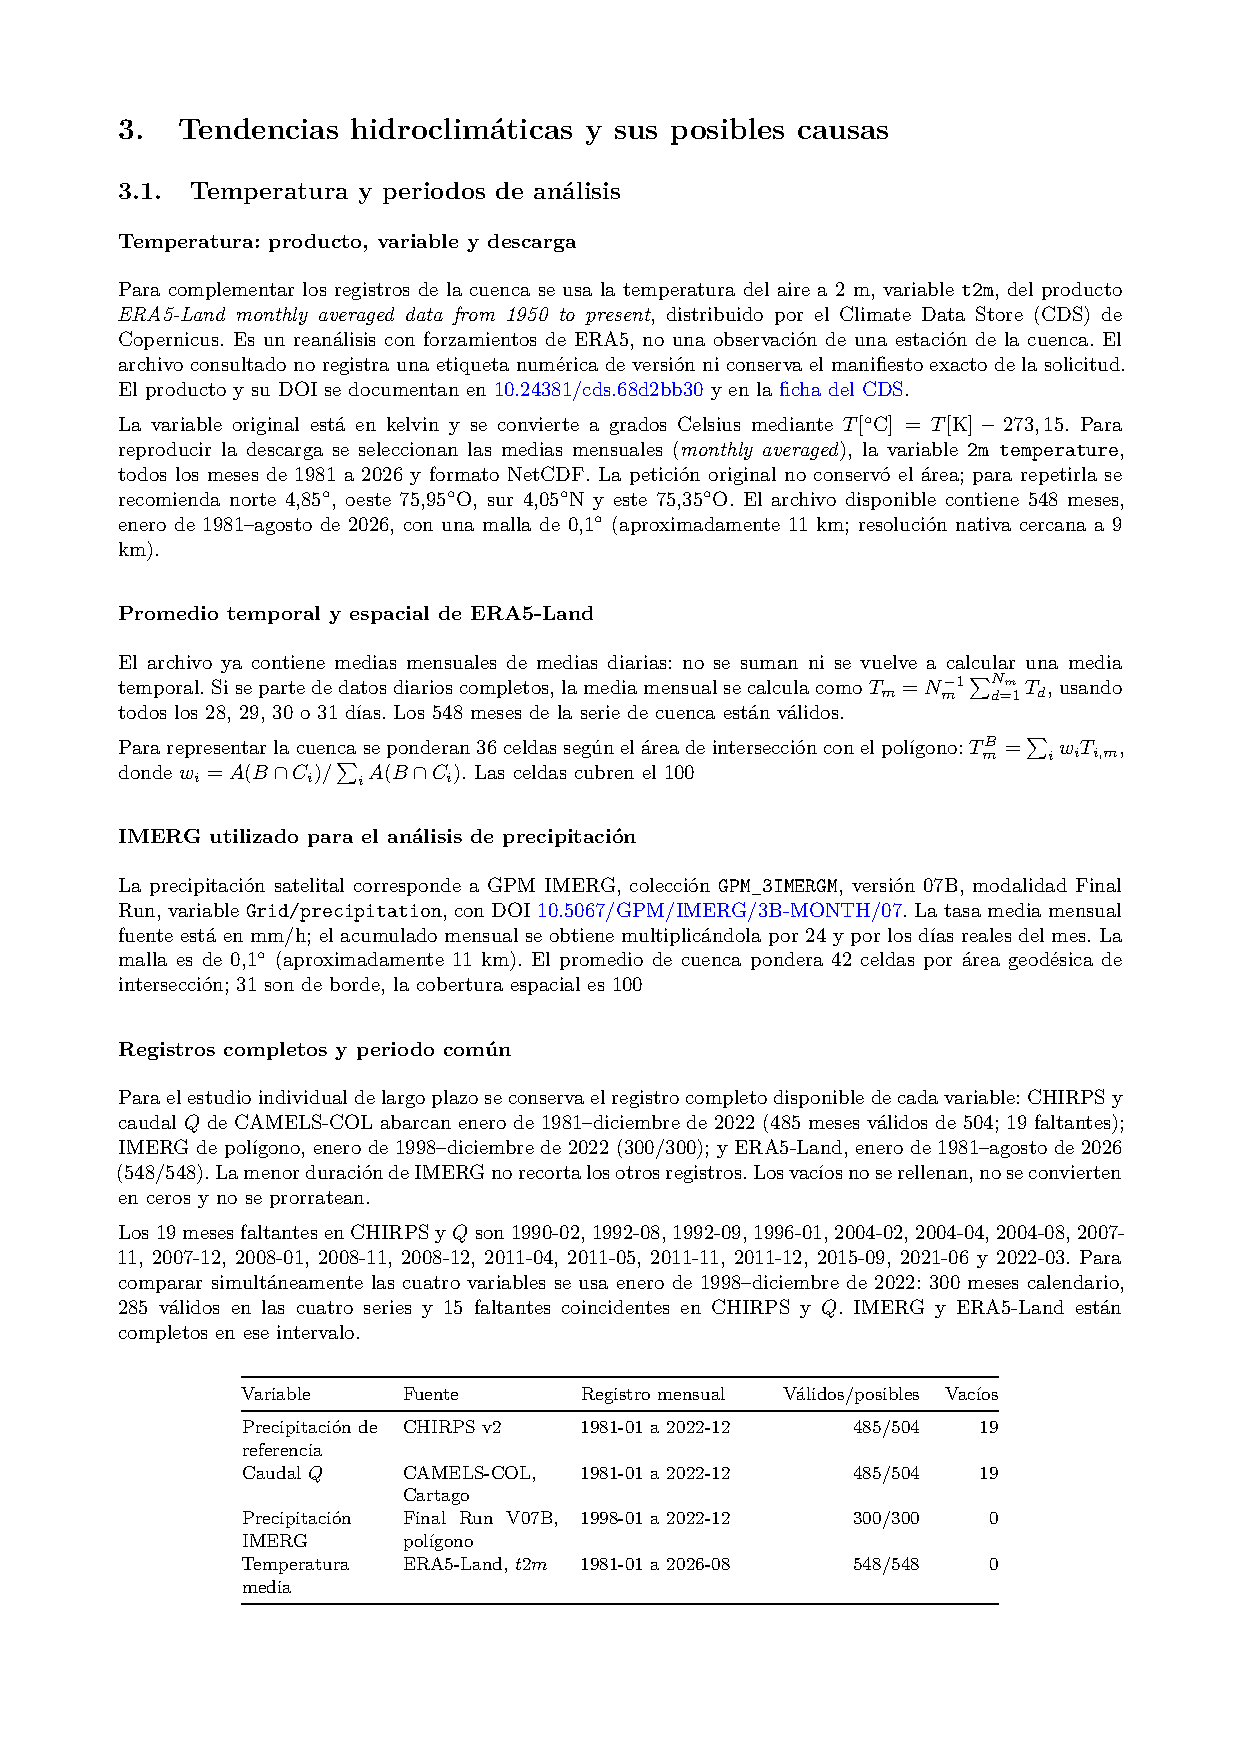
\includepdf[pages=-,pagecommand={\thispagestyle{plain}},addtotoc={
1,section,1,Tendencias hidroclimáticas y sus posibles causas,punto3,
1,subsection,2,Temperatura y periodos de análisis,punto31,
2,subsection,2,{Series originales, anomalías y anomalías estandarizadas},punto32,
4,subsection,2,Dos escalas de evaluación temporal,punto33,
6,subsection,2,Métodos y comparación de resultados,punto34,
9,subsection,2,{Incertidumbre, robustez y presentación},punto35,
10,subsection,2,Interpretación física de la variabilidad hidroclimática,punto36
}]{../apartado_3/punto_3_commit_2d27402.pdf}
% PUNTO_3_COMMIT_2D27402_FIN
\section{Análisis de frecuencias mediante Fourier}
\subsection{Preparar las series y documentar el cálculo}
Pendiente de desarrollar.
\subsection{Construir e interpretar los espectros}
Pendiente de desarrollar.
\clearpage
\section{Mapas de correlación con el clima global}
\subsection{Seleccionar los campos climáticos}
\subsubsection*{Selección y justificación física}
Se obtuvo una base pública de campos globales mensuales: SST NOAA ERSSTv5, presión al nivel del mar (SLP) y altura geopotencial a 500 hPa (Z500) de NCEP/NCAR Reanalysis 1. Se añade presión de superficie como control vertical. La malla nativa de 2$^\circ$/2,5$^\circ$ resuelve patrones de gran escala y evita interpolar a una resolución aparente mayor. No resuelve el relieve ni los procesos de lluvia de una cuenca andina. La selección se fijó antes de calcular mapas de correlación.

\subsubsection*{Mecanismos relevantes y alcance}
Para el occidente y los Andes colombianos, la literatura describe conexiones de la lluvia con SST del Pacífico y Atlántico, ENSO y circulación asociada a los chorros de Chocó y del Caribe (Poveda y Mesa, 1997; Poveda et al., 2014). Es una justificación regional, no una atribución demostrada para La Vieja. SLP y Z500 describen el estado de circulación; para evaluar directamente advección de humedad se necesitarían vientos y humedad, no inferirla solo de estos dos campos.

\subsubsection*{Productos atmosféricos y alternativas}
Se consideraron los productos mensuales ERA5 en superficie y en niveles de presión, distribuidos por el CDS en una malla atmosférica regular de 0,25$^\circ$. En este análisis se adopta NCEP/NCAR Reanalysis 1, de acceso público y resolución de 2,5$^\circ$, como base inicial para identificar patrones de gran escala. ERA5 constituye una alternativa para evaluar la sensibilidad de los resultados al reanálisis y a la resolución espacial; esa comparación requeriría una agregación consistente por área y debe conservar ambos productos separados. La temperatura ERA5-Land utilizada en el estudio de cuenca no reemplaza los campos atmosféricos globales.

\subsubsection*{Periodo, cobertura y correspondencia con la cuenca}
Cada campo descargado contiene 504 meses consecutivos entre enero de 1981 y diciembre de 2022. CHIRPS y Q tienen 485 meses completos; IMERG tiene 300 desde 1998. La comparación principal conserva los mismos 285 meses completos de CHIRPS, IMERG y Q en 1998-2022, con 15 huecos sin relleno. El análisis secundario CHIRPS-Q podrá usar 1981-2022 por separado. La muestra principal aporta entre 22 y 25 pares por mes calendario; los mapas informarán el tamaño efectivo en cada píxel.

\subsubsection*{Unidades, máscaras y transformaciones}
Las medias mensuales no se suman. SLP y presión superficial vienen en las unidades declaradas en el NetCDF: se dividen por 100 solo si están en Pa; millibars equivale a hPa. NCEP hgt ya es altura geopotencial en metros: no se vuelve a dividir por g. En ERA5, geopotential es $\Phi$ en m$^2$/s$^2$ y se convertiría a Z=$\Phi$/9,80665 m. Se conservan los faltantes oceánicos/terrestres de ERSST sin interpolarlos. Las longitudes se normalizan a [-180$^\circ$,180$^\circ$) sin duplicar la costura; cada campo mantiene su malla nativa.

\subsubsection*{Control vertical y máscara para los mapas}
Se comparó cada celda y mes de presión superficial con 500 hPa: se enmascaran 24 valores celda-mes de Z500 donde la presión superficial mensual es menor de 500 hPa. Es un control sobre medias, no garantiza que el nivel esté sobre el terreno durante cada instante del mes. Los mapas por mes calendario deberán conservar solo píxeles con al menos 20 pares y variación no nula. SLP es una reducción al nivel del mar y puede ser menos fiable sobre terreno elevado; se contrastarán sus patrones sobre océanos y tierras altas en 5.3. Los valores de SST próximos a congelación y el hielo marino requieren cautela; el interés físico principal es tropical.

\subsubsection*{Anomalías y muestra de análisis}
Las anomalías de cada campo se definen como la diferencia entre el valor mensual y la media de su mes calendario. La climatología de referencia se estima con las mismas 285 fechas completas de la cuenca durante 1998-2022, de modo que las comparaciones no dependan de calendarios distintos. Los campos conservan su malla nativa, sus unidades y sus faltantes; no se elimina la tendencia. La verificación de una media de anomalías próxima a cero en cada mes confirma esta transformación. Los índices Niño 3.4 u ONI podrán complementar la interpretación, sin sustituir los campos espaciales. La asociación con lluvia y caudal, sus rezagos y su robustez se evaluarán en los apartados siguientes.

\subsubsection*{Procedencia y alcance de los productos}
La base global combina ERSSTv5 y NCEP/NCAR Reanalysis 1, distribuidos por NOAA PSL. ERSSTv5 es una reconstrucción de SST basada en observaciones oceánicas, mientras que los campos atmosféricos proceden de un reanálisis; por ello, sus valores no se interpretan como mediciones locales directas. Se fijaron las versiones, el periodo y los niveles verticales antes de construir los mapas. Los metadatos de soporte conservan las solicitudes de acceso, fechas, coordenadas, unidades y huellas SHA-256 de los archivos, junto con los conteos y las máscaras. La lluvia de Zaragoza no se utiliza como respuesta principal: sus 14 meses completos resultan insuficientes para estimar asociaciones por mes calendario.

\begin{figure}[H]\centering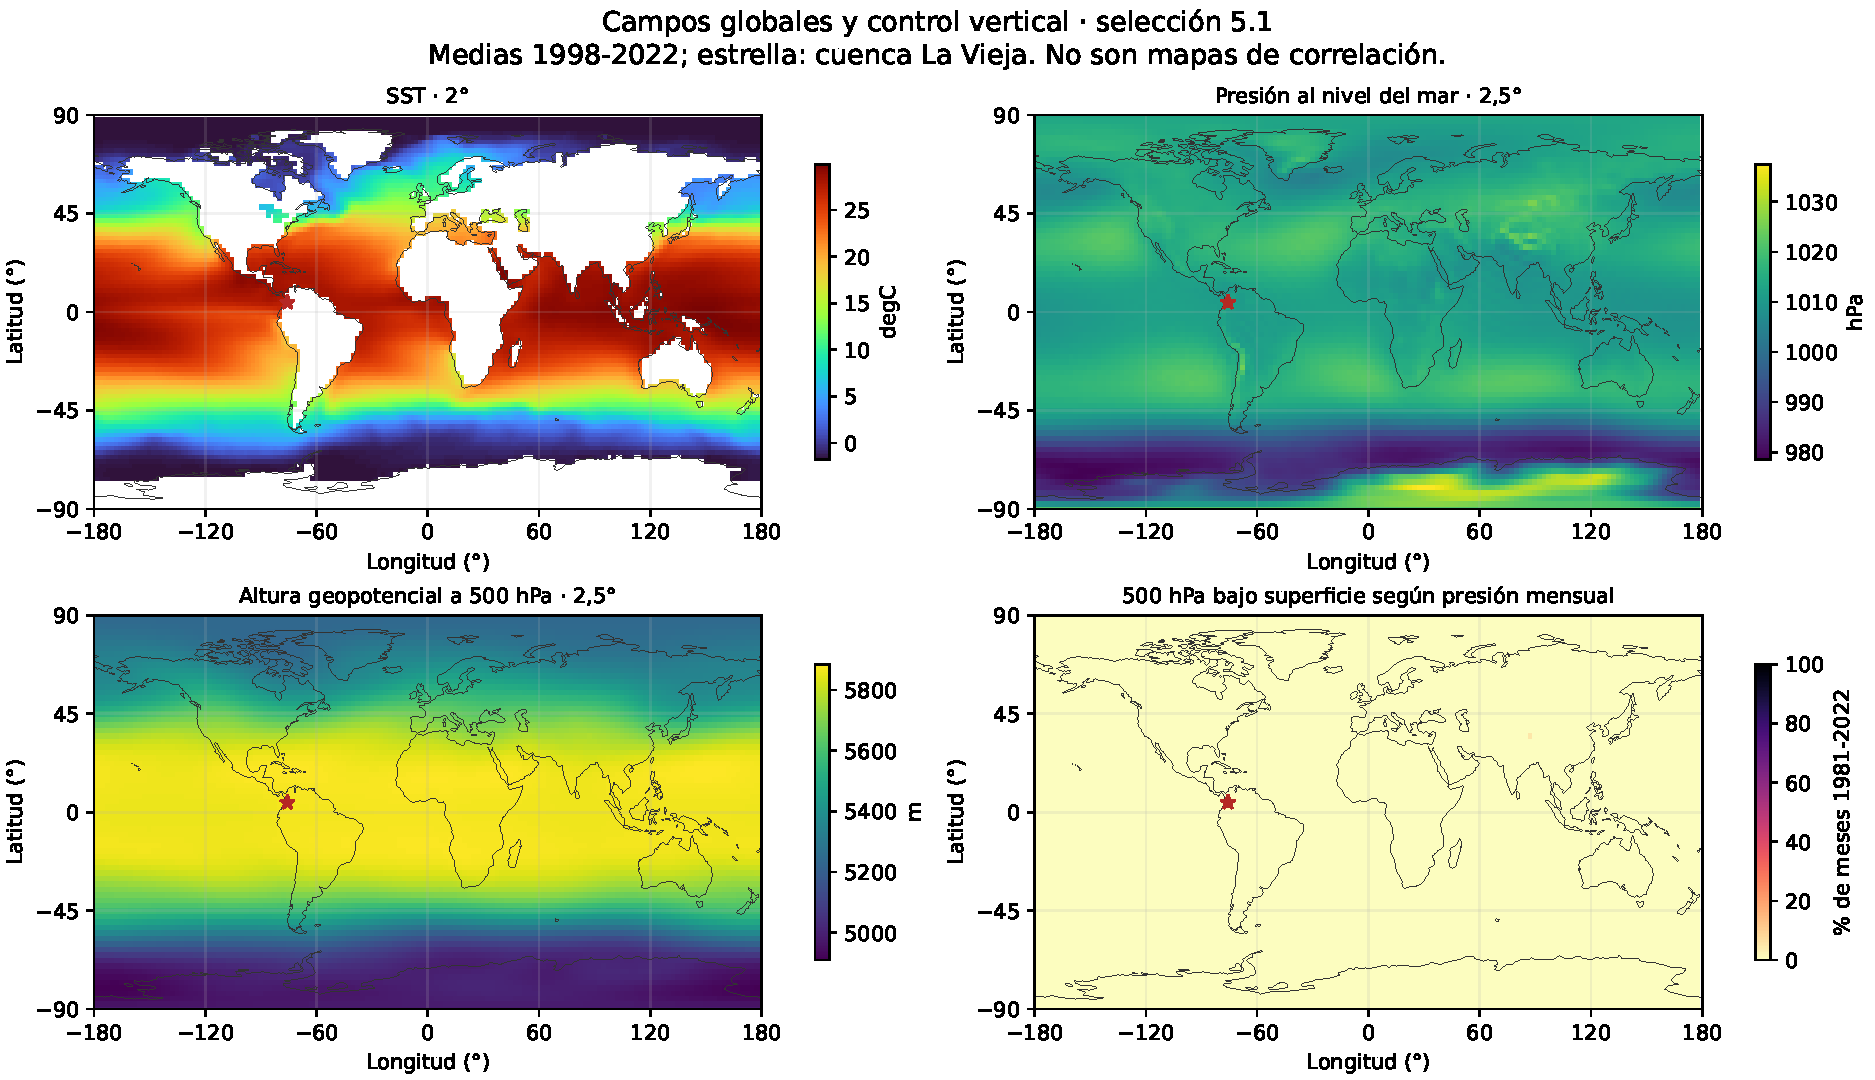
\includegraphics[width=\linewidth]{../apartado_5_1/campos_globales_control.pdf}\caption{Campos obtenidos y control vertical; no son mapas de correlación.}\end{figure}
\subsection{Definir y calcular los mapas mensuales}
\subsubsection*{Variabilidad interanual y definición de los mapas}
La asociación entre la hidroclimatología de La Vieja y los campos globales se estima mediante correlaciones temporales en cada celda. Para un mes calendario j se comparan los valores de la respuesta de cuenca en todos los años disponibles con los del campo climático correspondientes a ese mismo mes o al mes antecedente definido por el rezago. Cada combinación presenta doce mapas, uno por mes de la respuesta. Las correlaciones no se calculan entre celdas ni a partir de un único mes observado.

\subsubsection*{Respuestas de cuenca y fuentes}
La precipitación de referencia corresponde a CHIRPS, promediada sobre la cuenca; el caudal se observa en Cartago. IMERG Final Run V07B permite contrastar la sensibilidad de los patrones a la fuente de precipitación. CHIRPS es un producto espacial combinado, no una medición puntual independiente. La lluvia de Zaragoza dispone de solo 14 meses completos y no permite estimar doce correlaciones interanuales; por ello, no se atribuyen los mapas a esa estación. Se emplean SST ERSSTv5, presión al nivel del mar y altura geopotencial a 500 hPa de NCEP/NCAR R1, manteniendo las rejillas y máscaras del 5.1.

\subsubsection*{Anomalías, rezagos y tamaño efectivo}
La referencia comprende las mismas 285 fechas completas de cuenca en 1998–2022. Para cada variable se resta la climatología de su mes calendario; los campos globales y las respuestas conservan sus unidades antes de calcular el coeficiente adimensional. La base tiene rezago cero. Para Q se añade un rezago de un mes como exploración de la persistencia climática y de una respuesta hidrológica con almacenamiento; no se interpreta como tiempo de concentración. Con la convención r\_j(lon,lat;ell) = corr[a\_X(t),a\_Y(lon,lat,t-ell)] para mes(t)=j, ell>0 significa que el campo climático antecede al caudal. Enero de 1998 se empareja con diciembre de 1997 para ell=1. El desplazamiento se hace en el calendario completo; no se usan valores futuros ni se comprimen los huecos.

\subsubsection*{Criterios de cálculo y representación}
Pearson es la referencia y Spearman contrasta la sensibilidad a extremos, asimetría y relaciones monotónicas no lineales. Spearman se calcula sobre rangos con promedio para empates y la misma máscara de pares válidos. Cada mapa informa el mínimo y máximo n de sus celdas representadas. Se exige n$\geq$20 y variación no nula en ambas variables; las celdas restantes se muestran grises. Las respuestas aportan entre 22 y 25 años por mes, no 285 observaciones para cada enero. Los campos globales están completos en el calendario seleccionado y el antecedente de diciembre de 1997 está disponible; solo las máscaras de cada celda pueden reducir sus pares. Esta muestra no es la de 274 fechas de los modelos de lluvia antecedente del punto 2, que además necesitaban precipitación de cuenca del mes previo.

\subsubsection*{Lectura física y alcance}
Un coeficiente negativo indica que anomalías positivas del campo coinciden con anomalías negativas de la respuesta; un coeficiente positivo indica desviaciones del mismo signo. La interpretación de SLP y Z500 corresponde a patrones de circulación de gran escala, no a mediciones directas de transporte de humedad. La concordancia entre Pearson y Spearman respalda una asociación menos dependiente de la escala o de unos pocos extremos, pero no demuestra causalidad ni constituye una prueba independiente. Los mapas de distintos meses, fuentes y métodos comparten años y forzamientos climáticos. No se eliminó tendencia ni se aplicaron pruebas de significancia: autocorrelación, pruebas múltiples y sensibilidad temporal se evaluarán en 5.3.

\subsubsection*{Contraste regional del Pacífico tropical}
Como apoyo a los mapas se construye un índice interno de anomalías SST en Niño 3.4 (5$^\circ$S–5$^\circ$N, 170$^\circ$W–120$^\circ$W), seleccionando centros de celda y ponderando por coseno de latitud. Es un promedio mensual sobre la referencia de este estudio, no el índice ONI ni su promedio móvil trimestral. Las correlaciones del índice con cada respuesta se calculan a través de los años de un mismo mes. Precipitación CHIRPS: r entre -0.58 y +0.04; negativo en 11/12 meses. Caudal Cartago: r entre -0.85 y -0.28; negativo en 12/12 meses. Precipitación IMERG: r entre -0.66 y -0.14; negativo en 12/12 meses. Estas cifras son descriptivas y no establecen significancia estadística; el detalle de los doce meses permite examinar la estacionalidad de la asociación sin seleccionar una sola celda extrema.

\subsubsection*{Sensibilidad de la precipitación frente a SST ERSSTv5}
La diferencia absoluta entre los mapas Pearson de CHIRPS e IMERG, promediada espacialmente con pesos de coseno de latitud, varía de 0.064 a 0.221 según el mes. Esta diferencia compara dos estimaciones de precipitación sobre las mismas fechas y rejillas; no mide precisión frente a una verdad observada ni es una correlación espacial de los datos. Los paneles permiten identificar si se conservan el signo y la extensión de los patrones, mientras que Spearman permite contrastar su sensibilidad a los rangos.

\subsubsection*{Sensibilidad de la precipitación frente a SLP NCEP/NCAR R1}
La diferencia absoluta entre los mapas Pearson de CHIRPS e IMERG, promediada espacialmente con pesos de coseno de latitud, varía de 0.062 a 0.191 según el mes. Esta diferencia compara dos estimaciones de precipitación sobre las mismas fechas y rejillas; no mide precisión frente a una verdad observada ni es una correlación espacial de los datos. Los paneles permiten identificar si se conservan el signo y la extensión de los patrones, mientras que Spearman permite contrastar su sensibilidad a los rangos.

\subsubsection*{Sensibilidad de la precipitación frente a Z500 NCEP/NCAR R1}
La diferencia absoluta entre los mapas Pearson de CHIRPS e IMERG, promediada espacialmente con pesos de coseno de latitud, varía de 0.080 a 0.273 según el mes. Esta diferencia compara dos estimaciones de precipitación sobre las mismas fechas y rejillas; no mide precisión frente a una verdad observada ni es una correlación espacial de los datos. Los paneles permiten identificar si se conservan el signo y la extensión de los patrones, mientras que Spearman permite contrastar su sensibilidad a los rangos.

\begin{figure}[p]\centering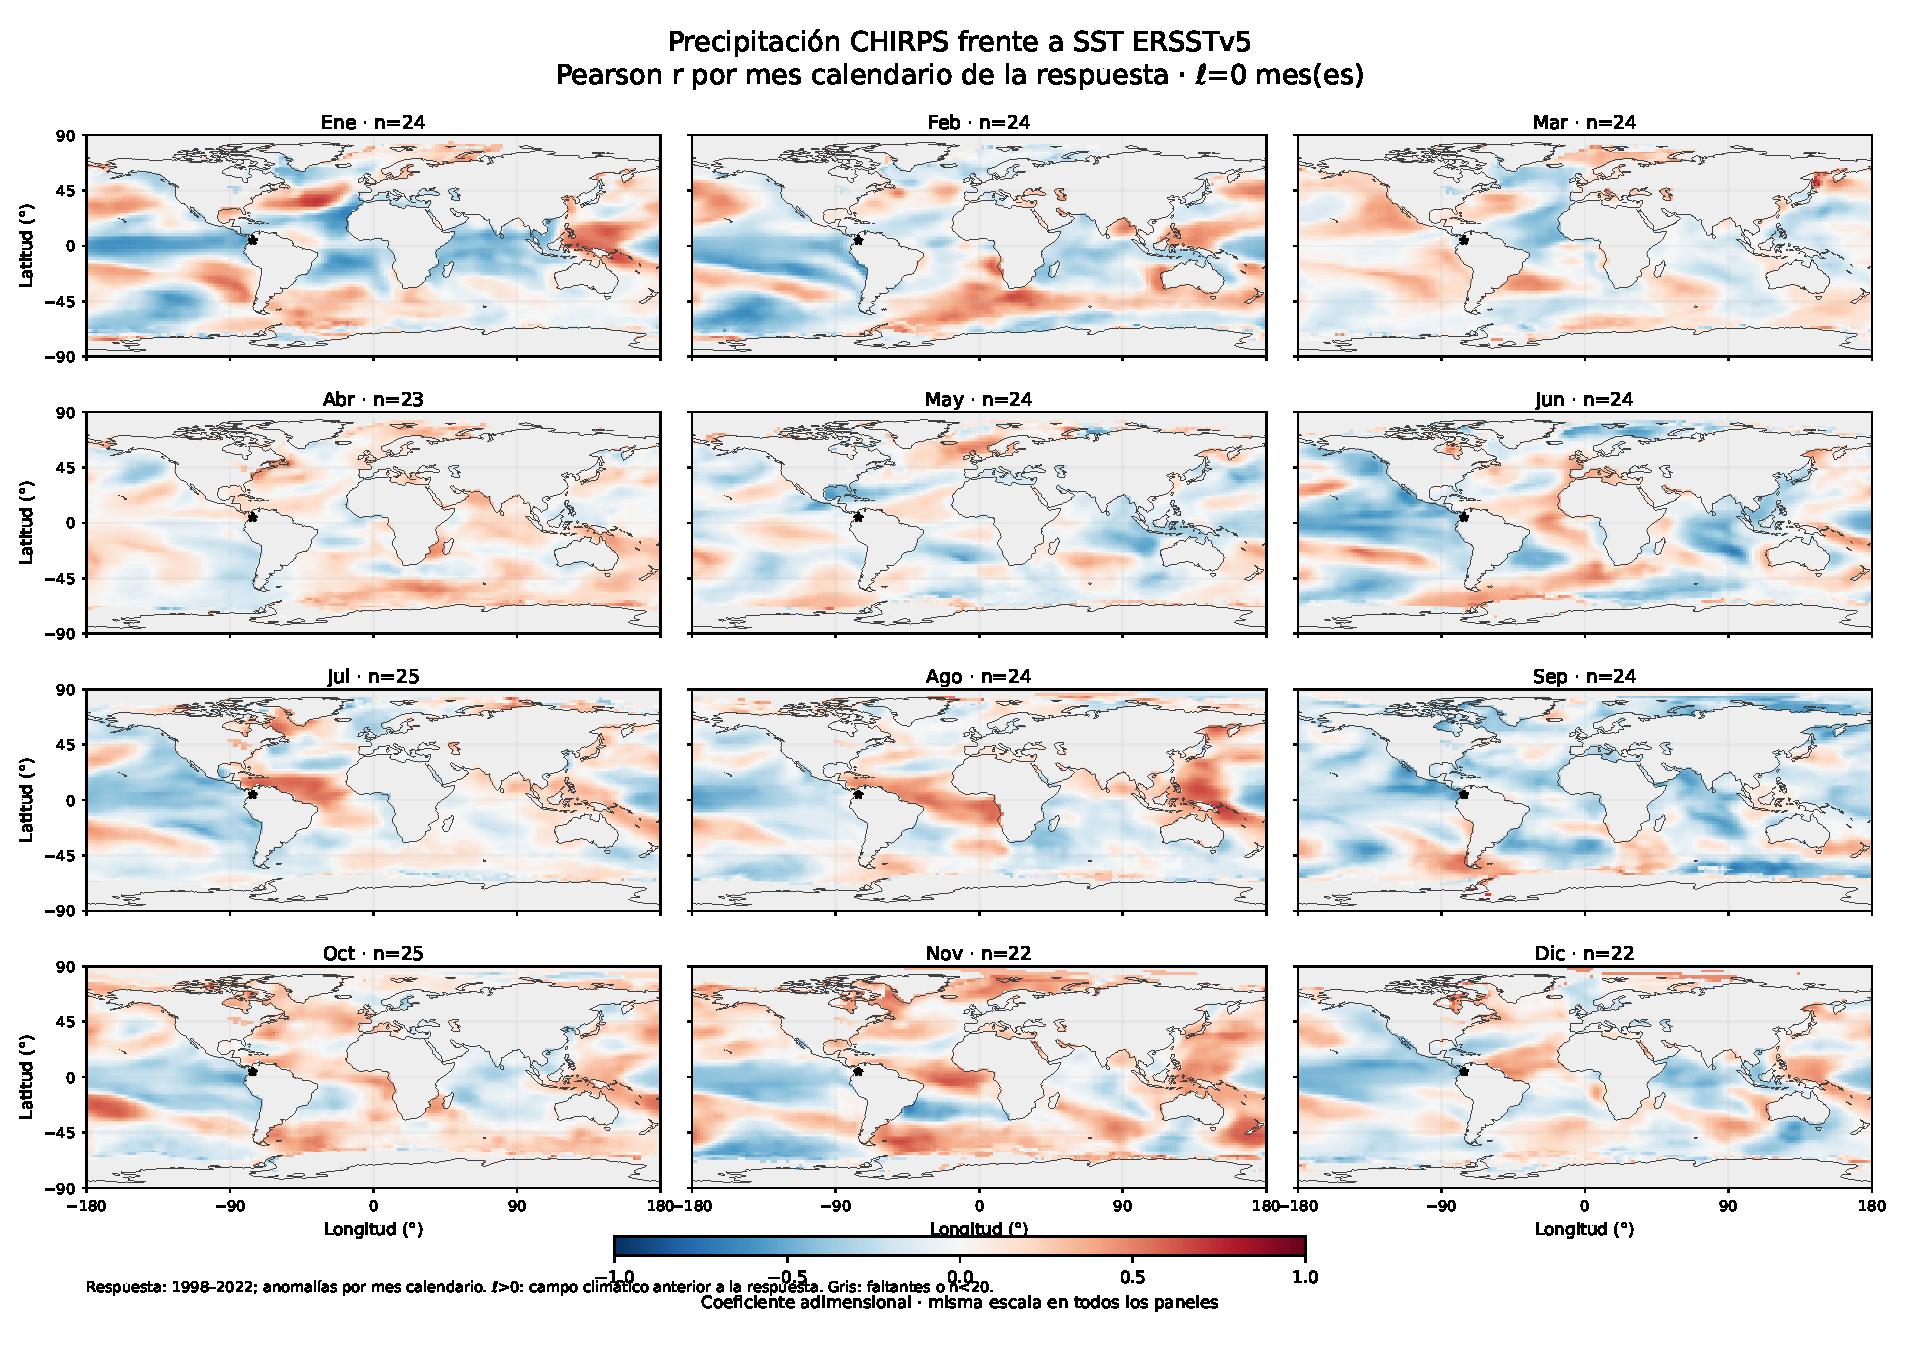
\includegraphics[width=\linewidth]{../apartado_5_2/CHIRPS_sst_l0_pearson.pdf}\caption{Doce correlaciones temporales por mes calendario; rezago 0 mes(es).}\end{figure}
\begin{figure}[p]\centering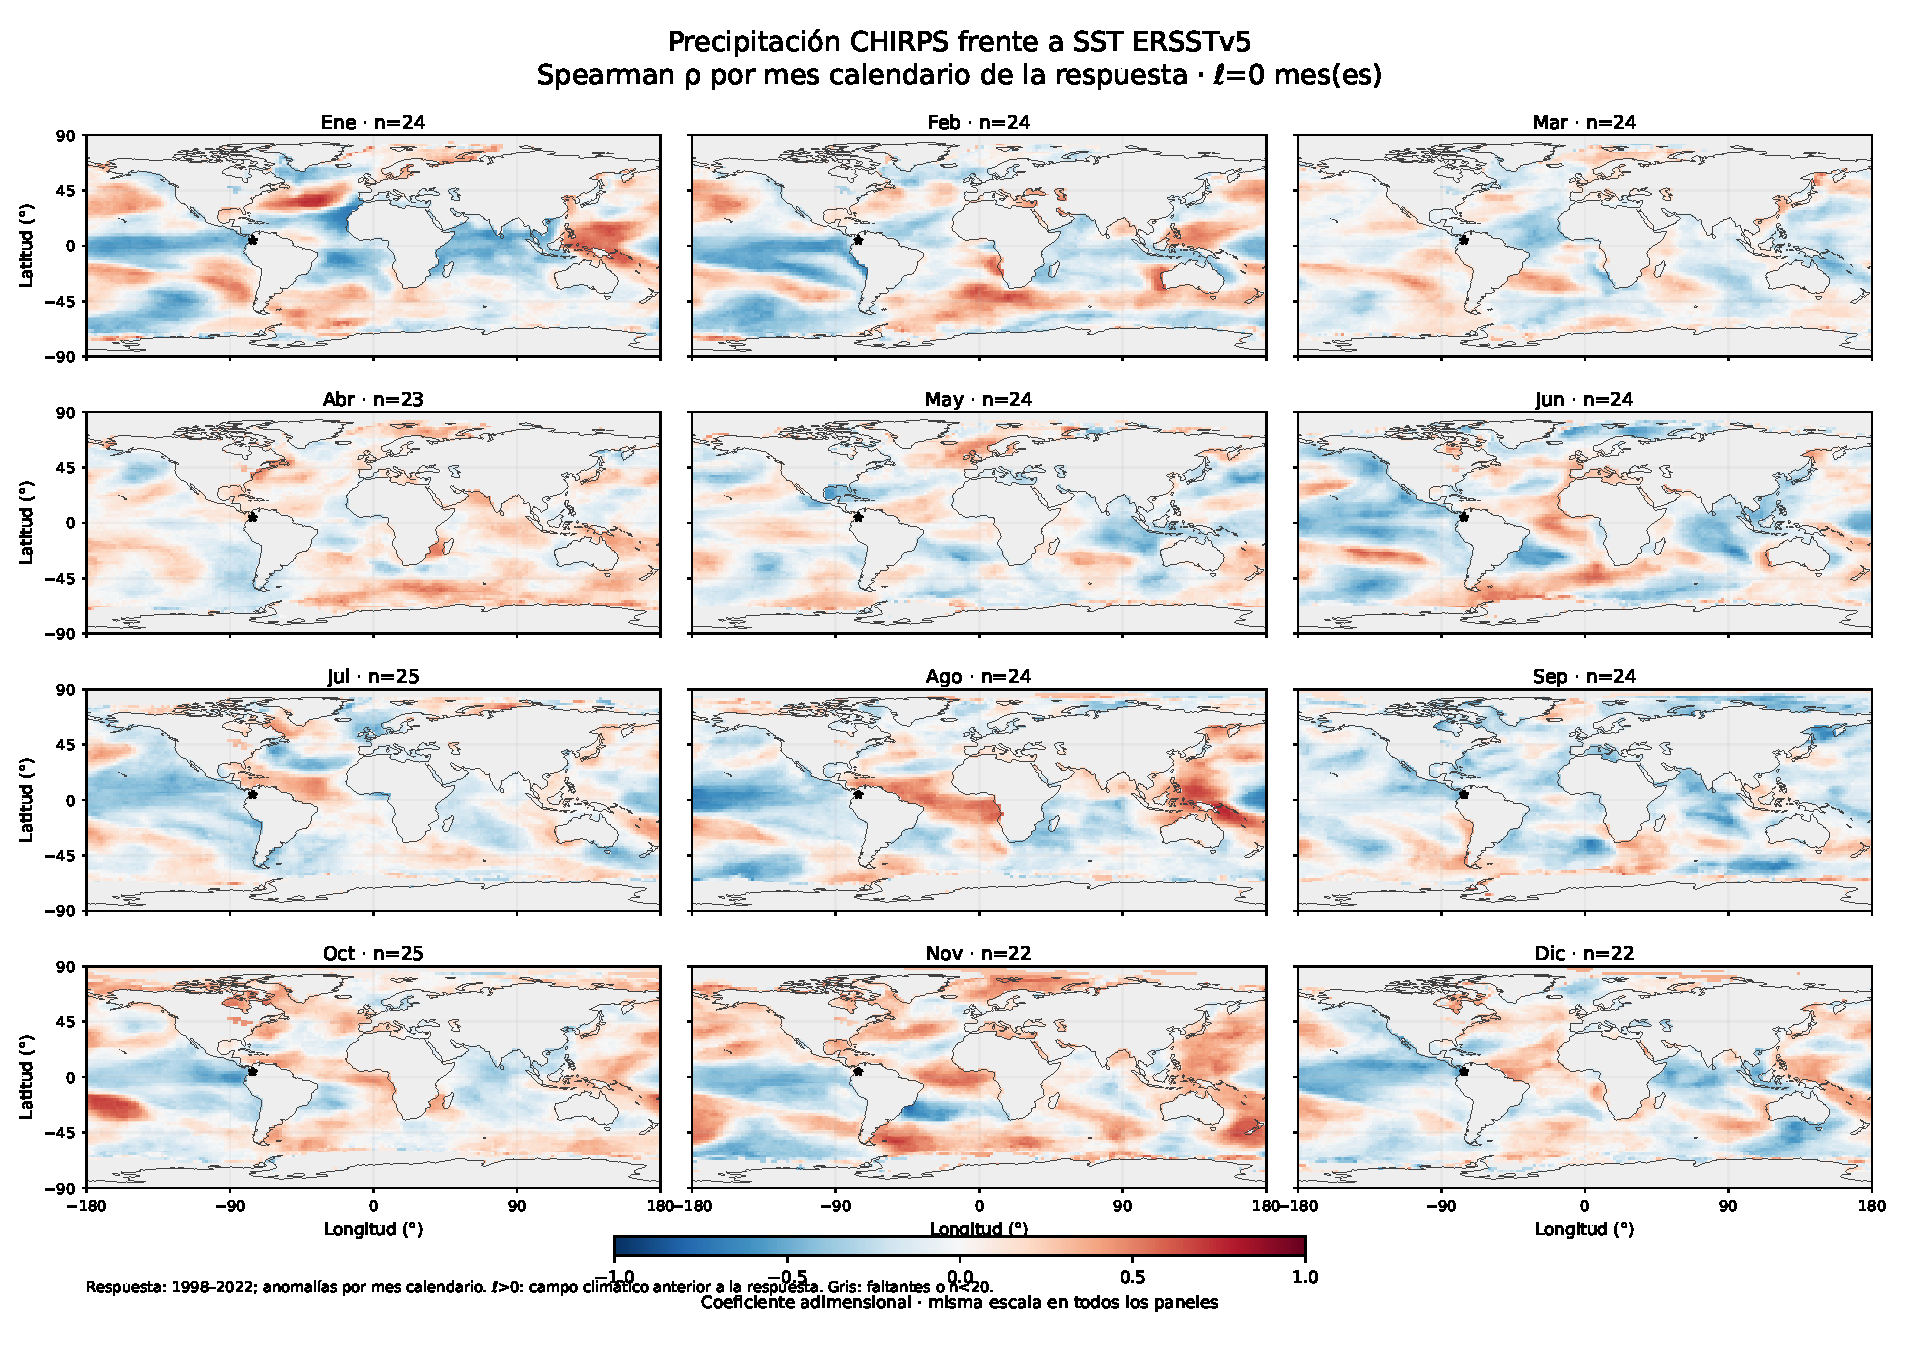
\includegraphics[width=\linewidth]{../apartado_5_2/CHIRPS_sst_l0_spearman.pdf}\caption{Doce correlaciones temporales por mes calendario; rezago 0 mes(es).}\end{figure}
\begin{figure}[p]\centering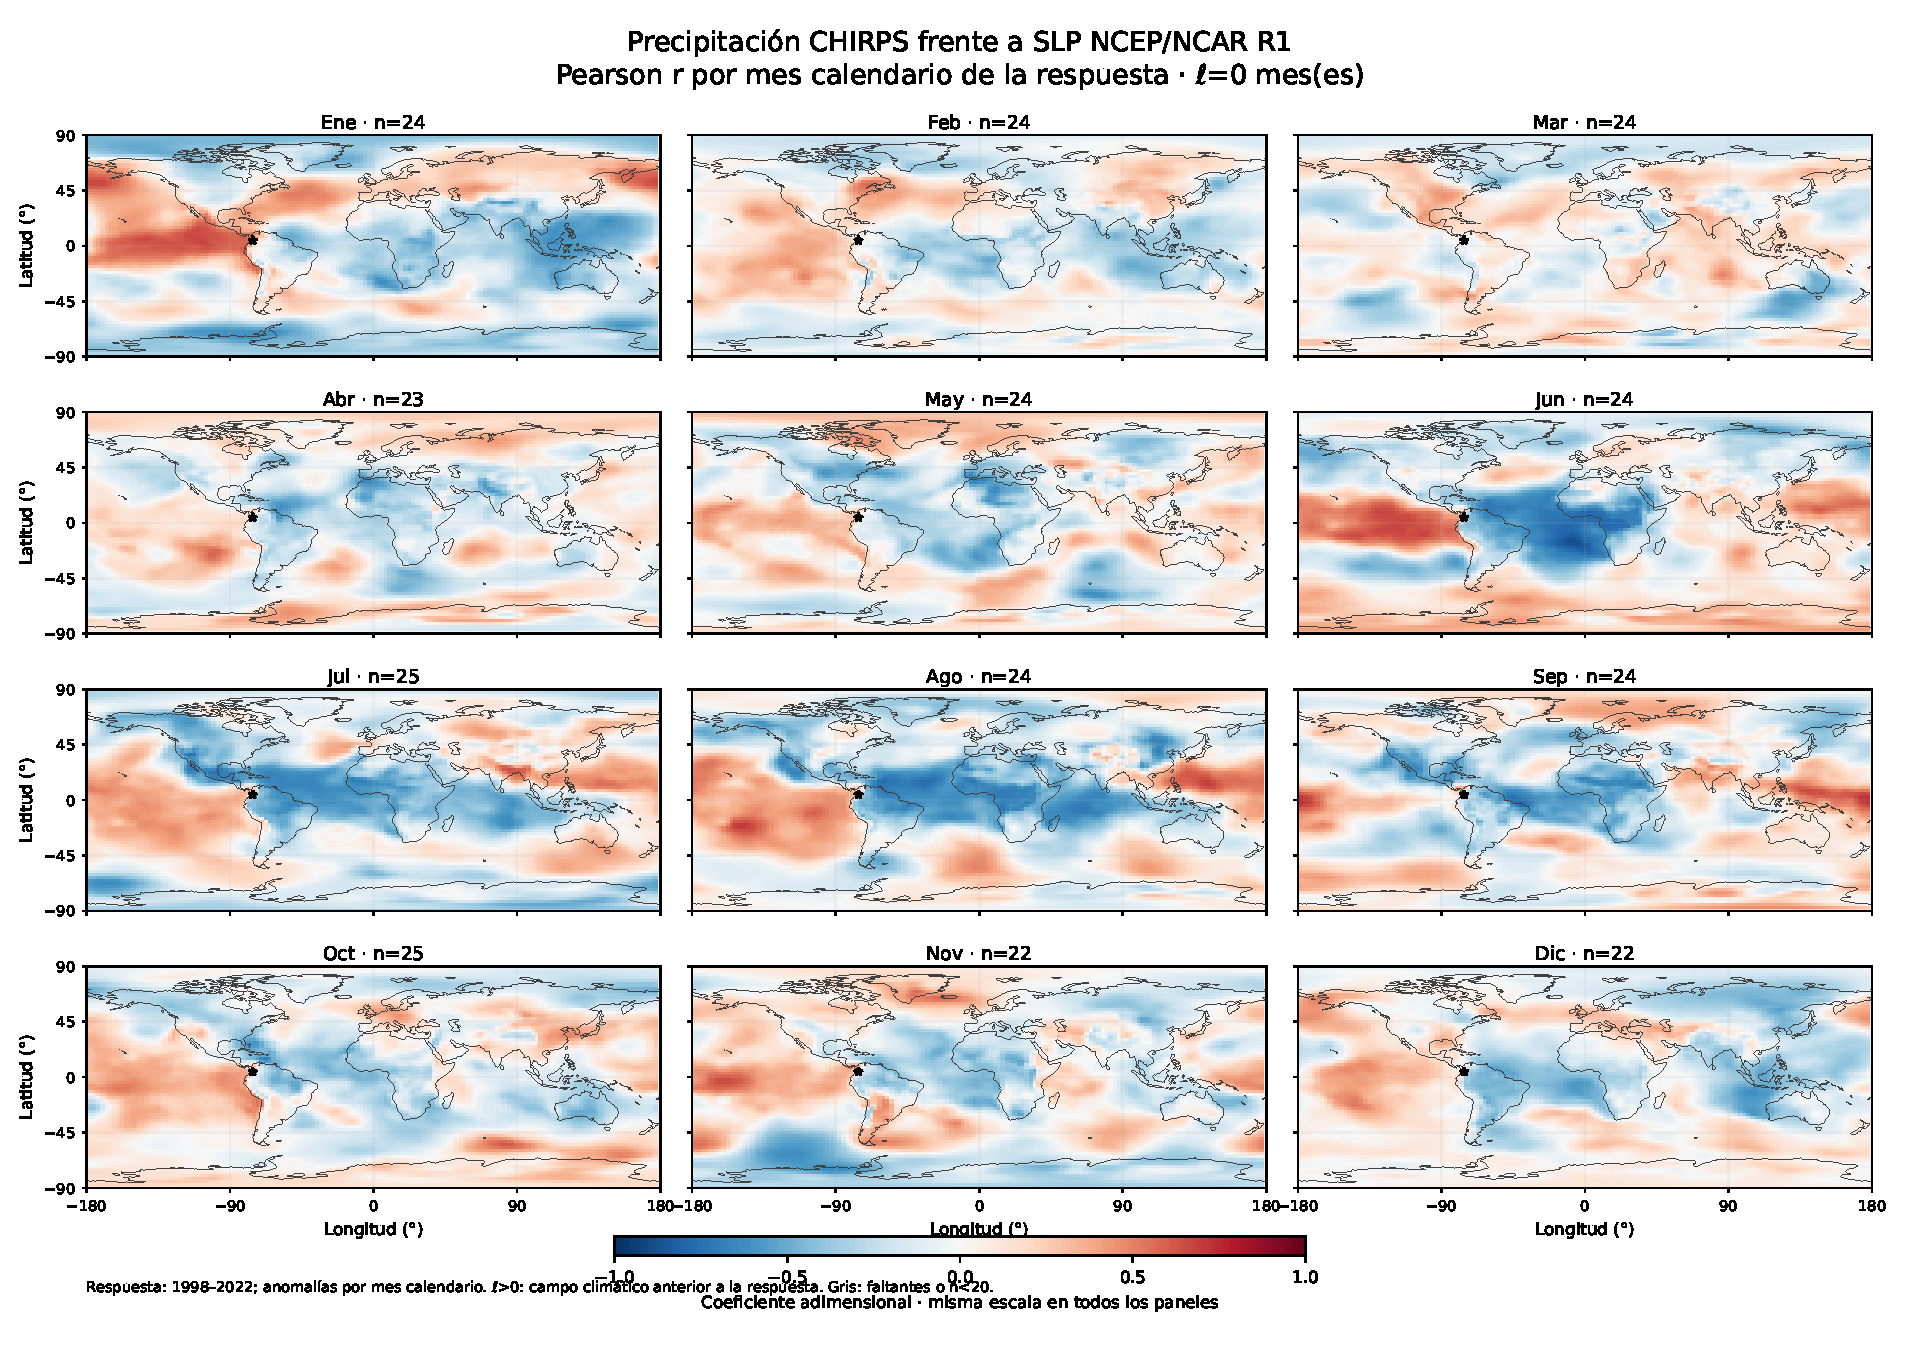
\includegraphics[width=\linewidth]{../apartado_5_2/CHIRPS_slp_l0_pearson.pdf}\caption{Doce correlaciones temporales por mes calendario; rezago 0 mes(es).}\end{figure}
\begin{figure}[p]\centering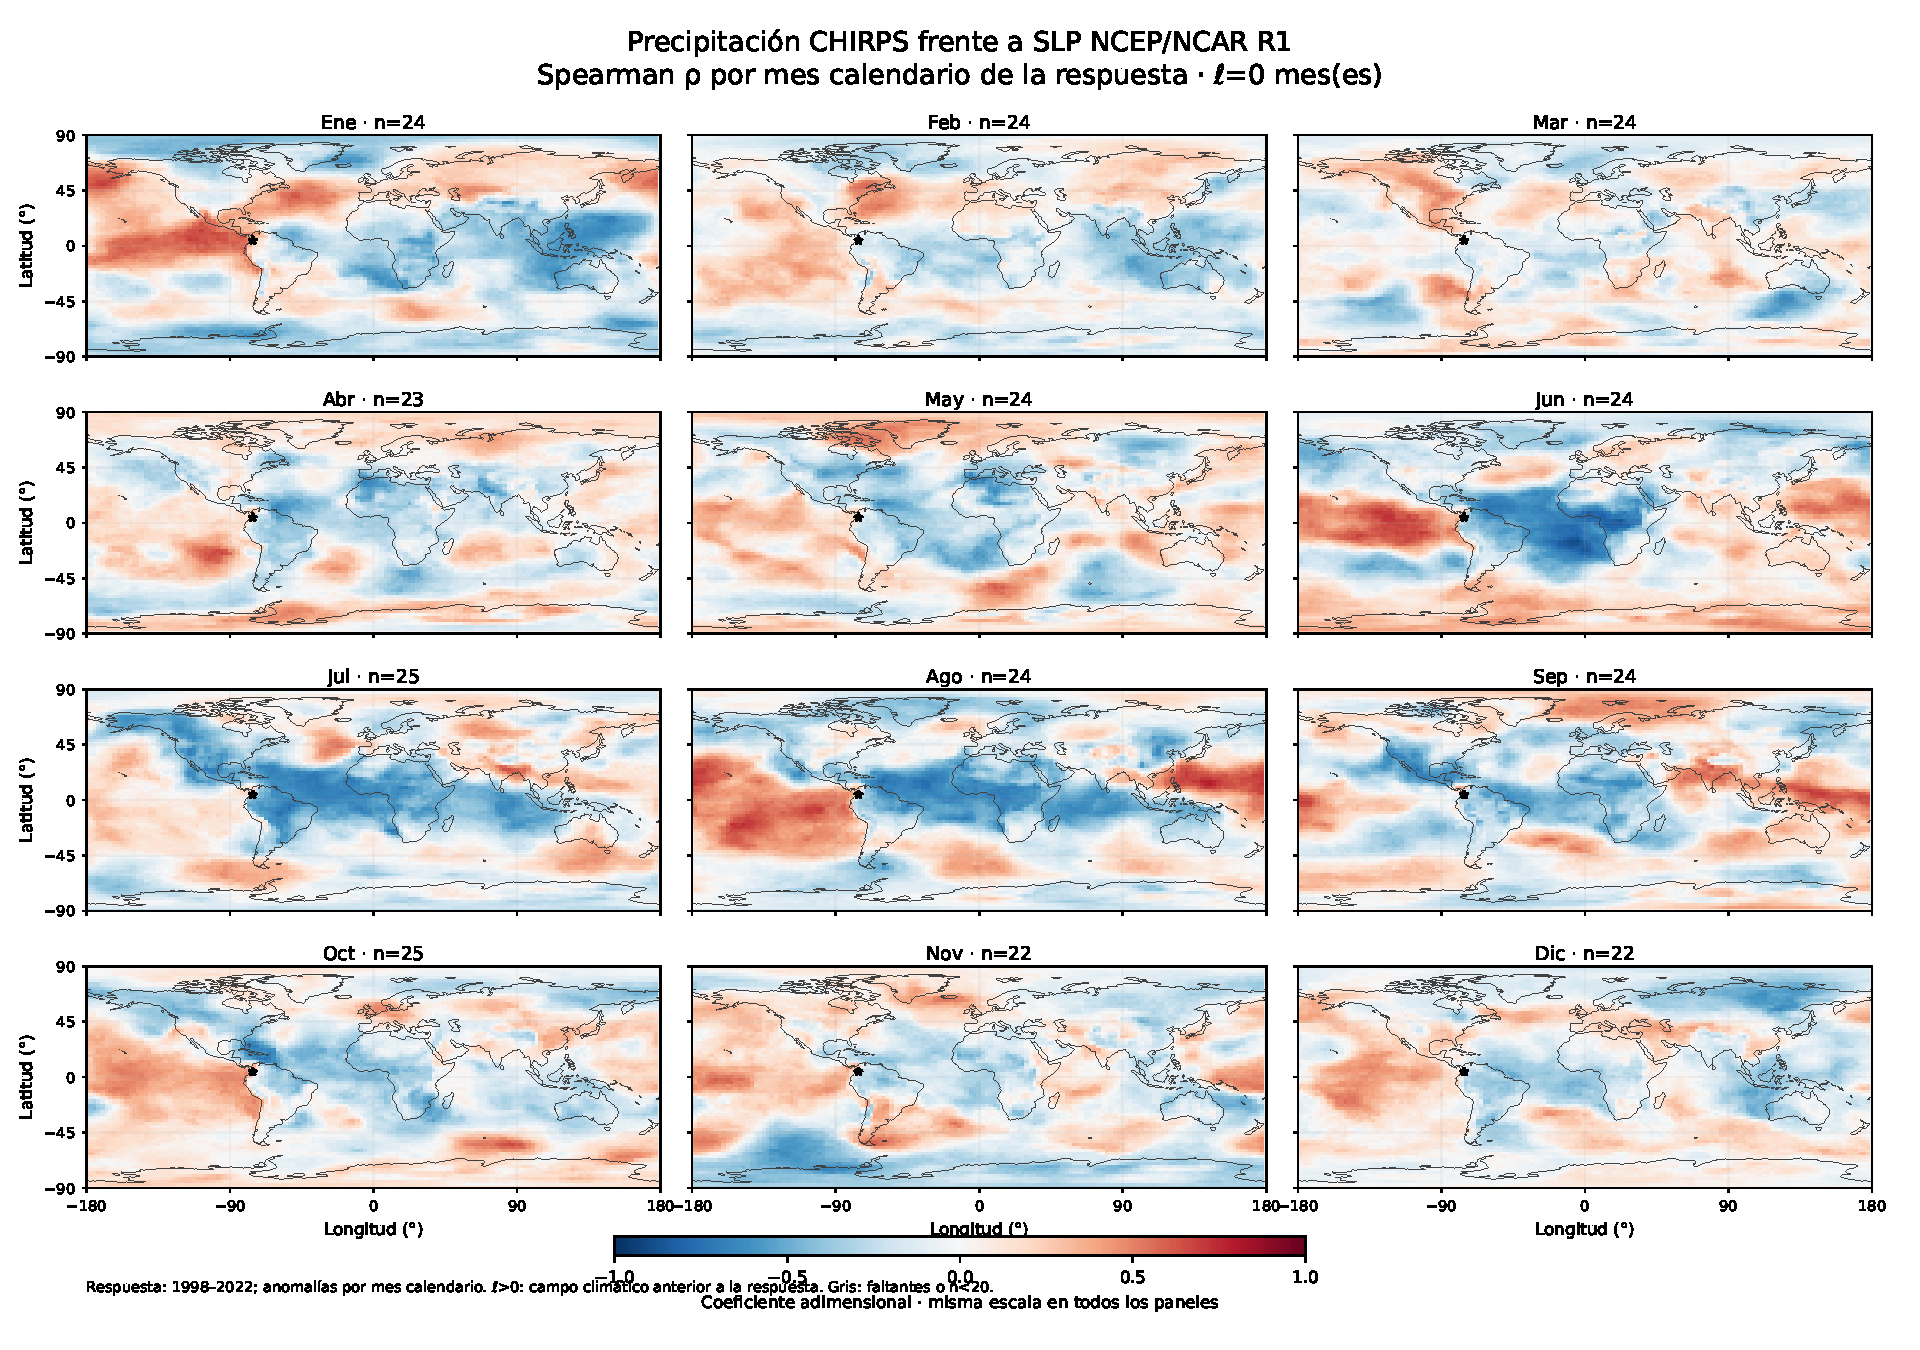
\includegraphics[width=\linewidth]{../apartado_5_2/CHIRPS_slp_l0_spearman.pdf}\caption{Doce correlaciones temporales por mes calendario; rezago 0 mes(es).}\end{figure}
\begin{figure}[p]\centering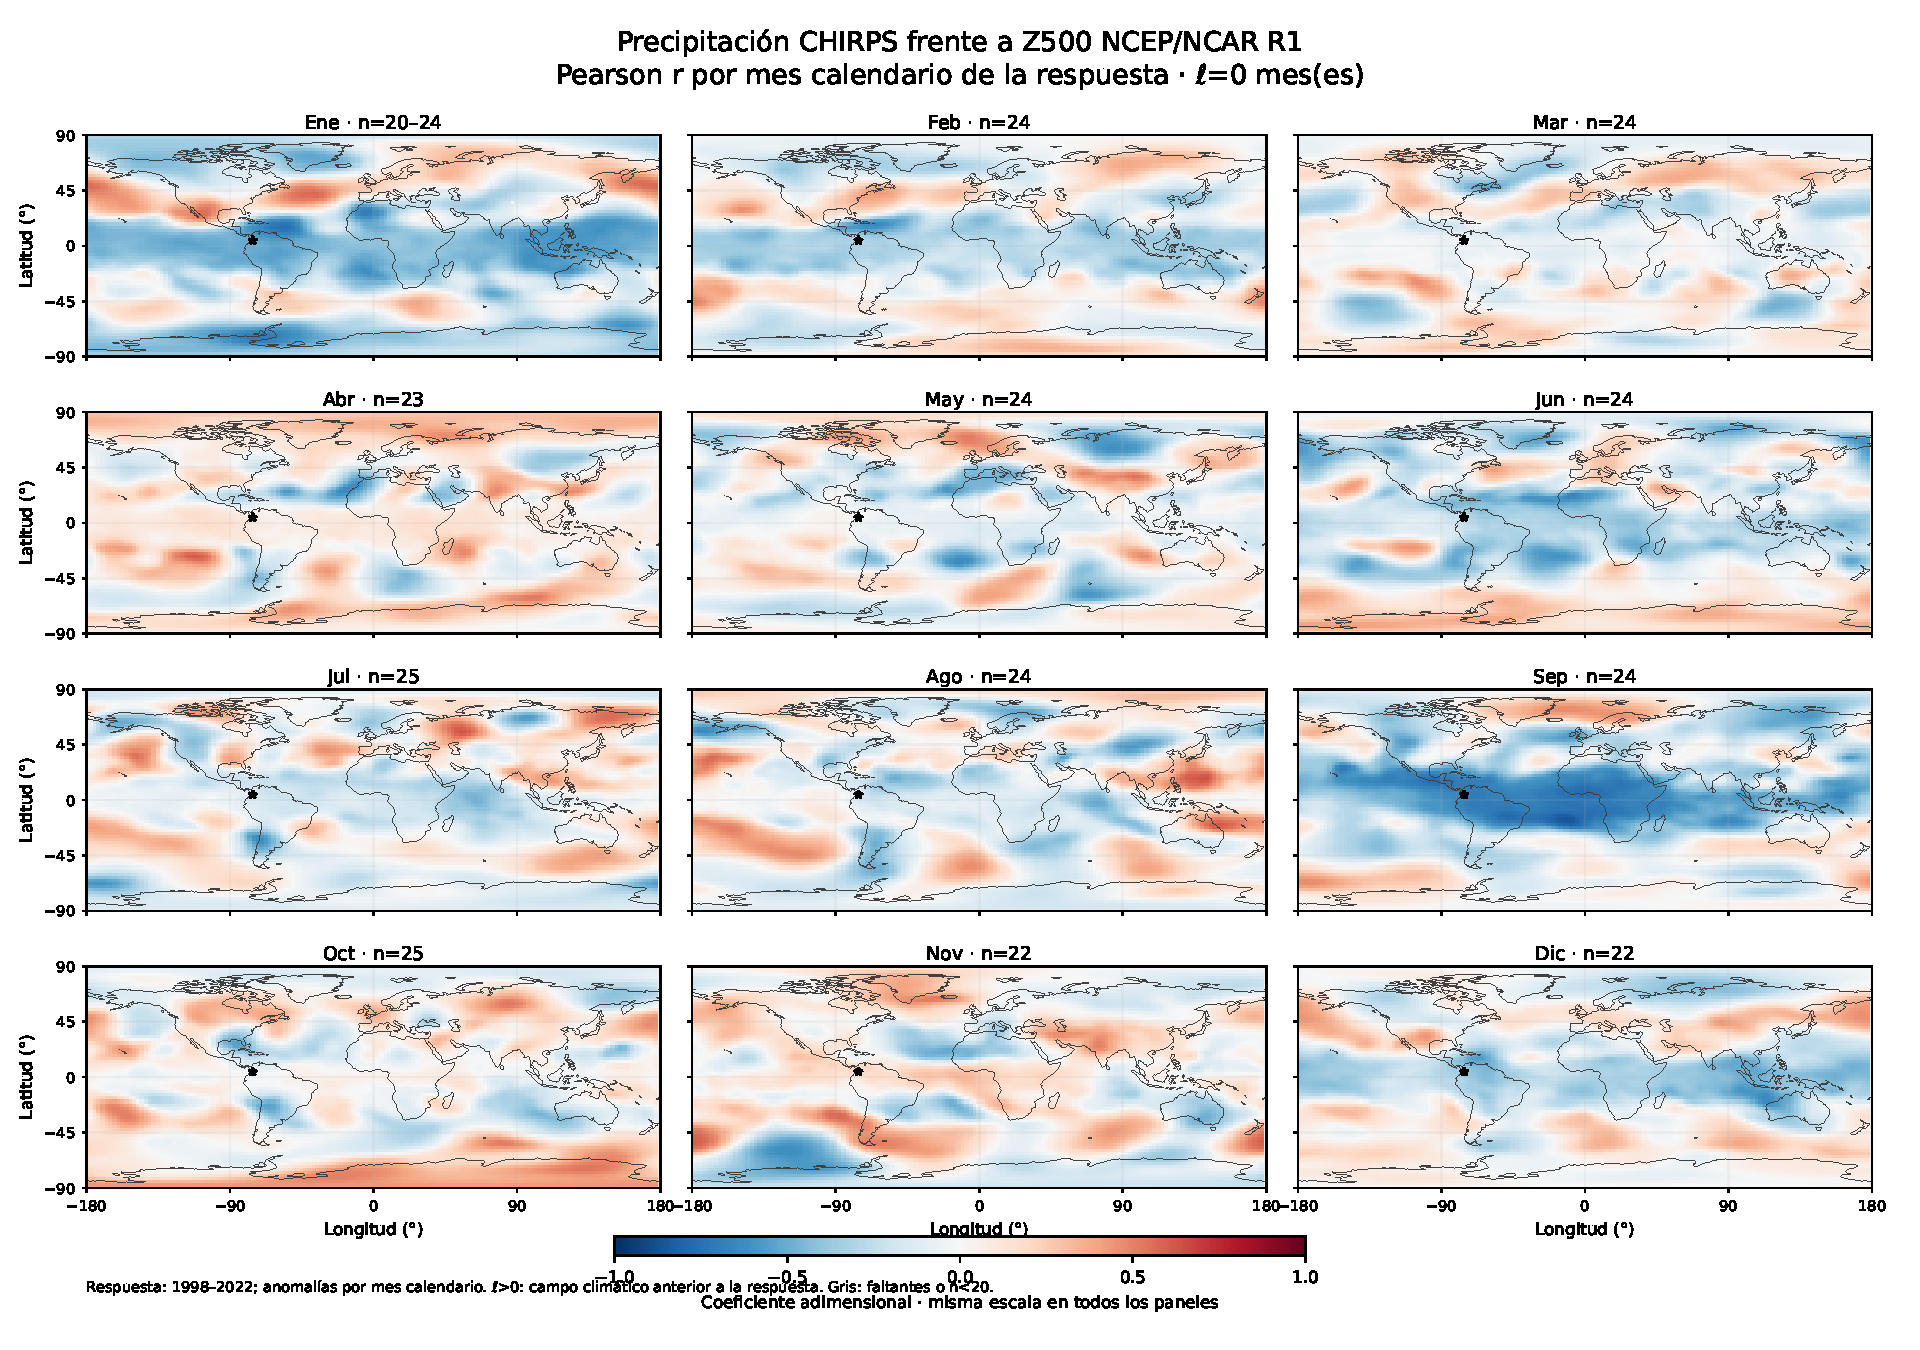
\includegraphics[width=\linewidth]{../apartado_5_2/CHIRPS_z500_l0_pearson.pdf}\caption{Doce correlaciones temporales por mes calendario; rezago 0 mes(es).}\end{figure}
\begin{figure}[p]\centering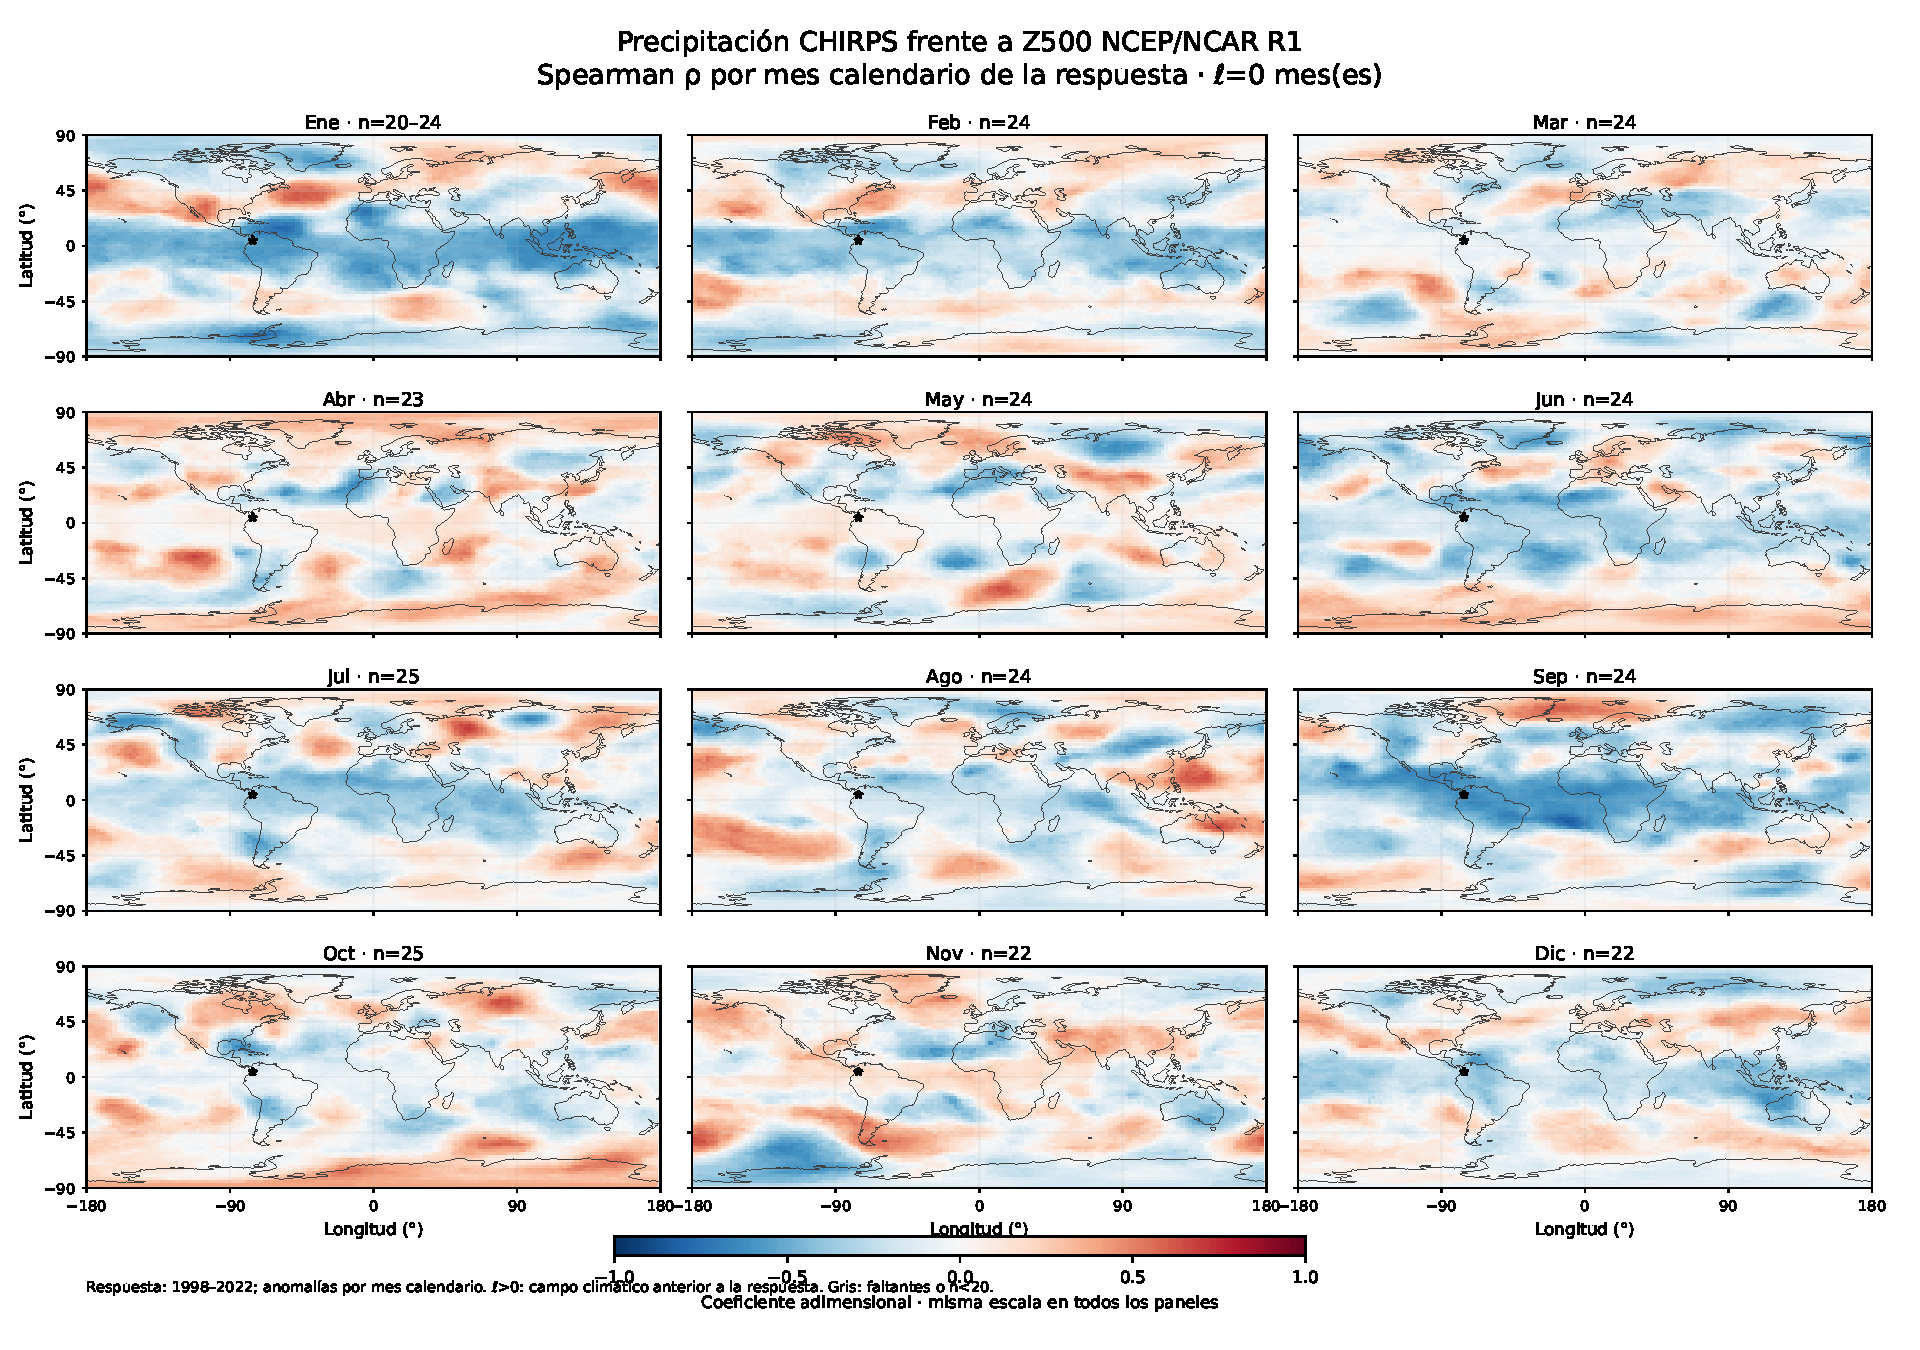
\includegraphics[width=\linewidth]{../apartado_5_2/CHIRPS_z500_l0_spearman.pdf}\caption{Doce correlaciones temporales por mes calendario; rezago 0 mes(es).}\end{figure}
\begin{figure}[p]\centering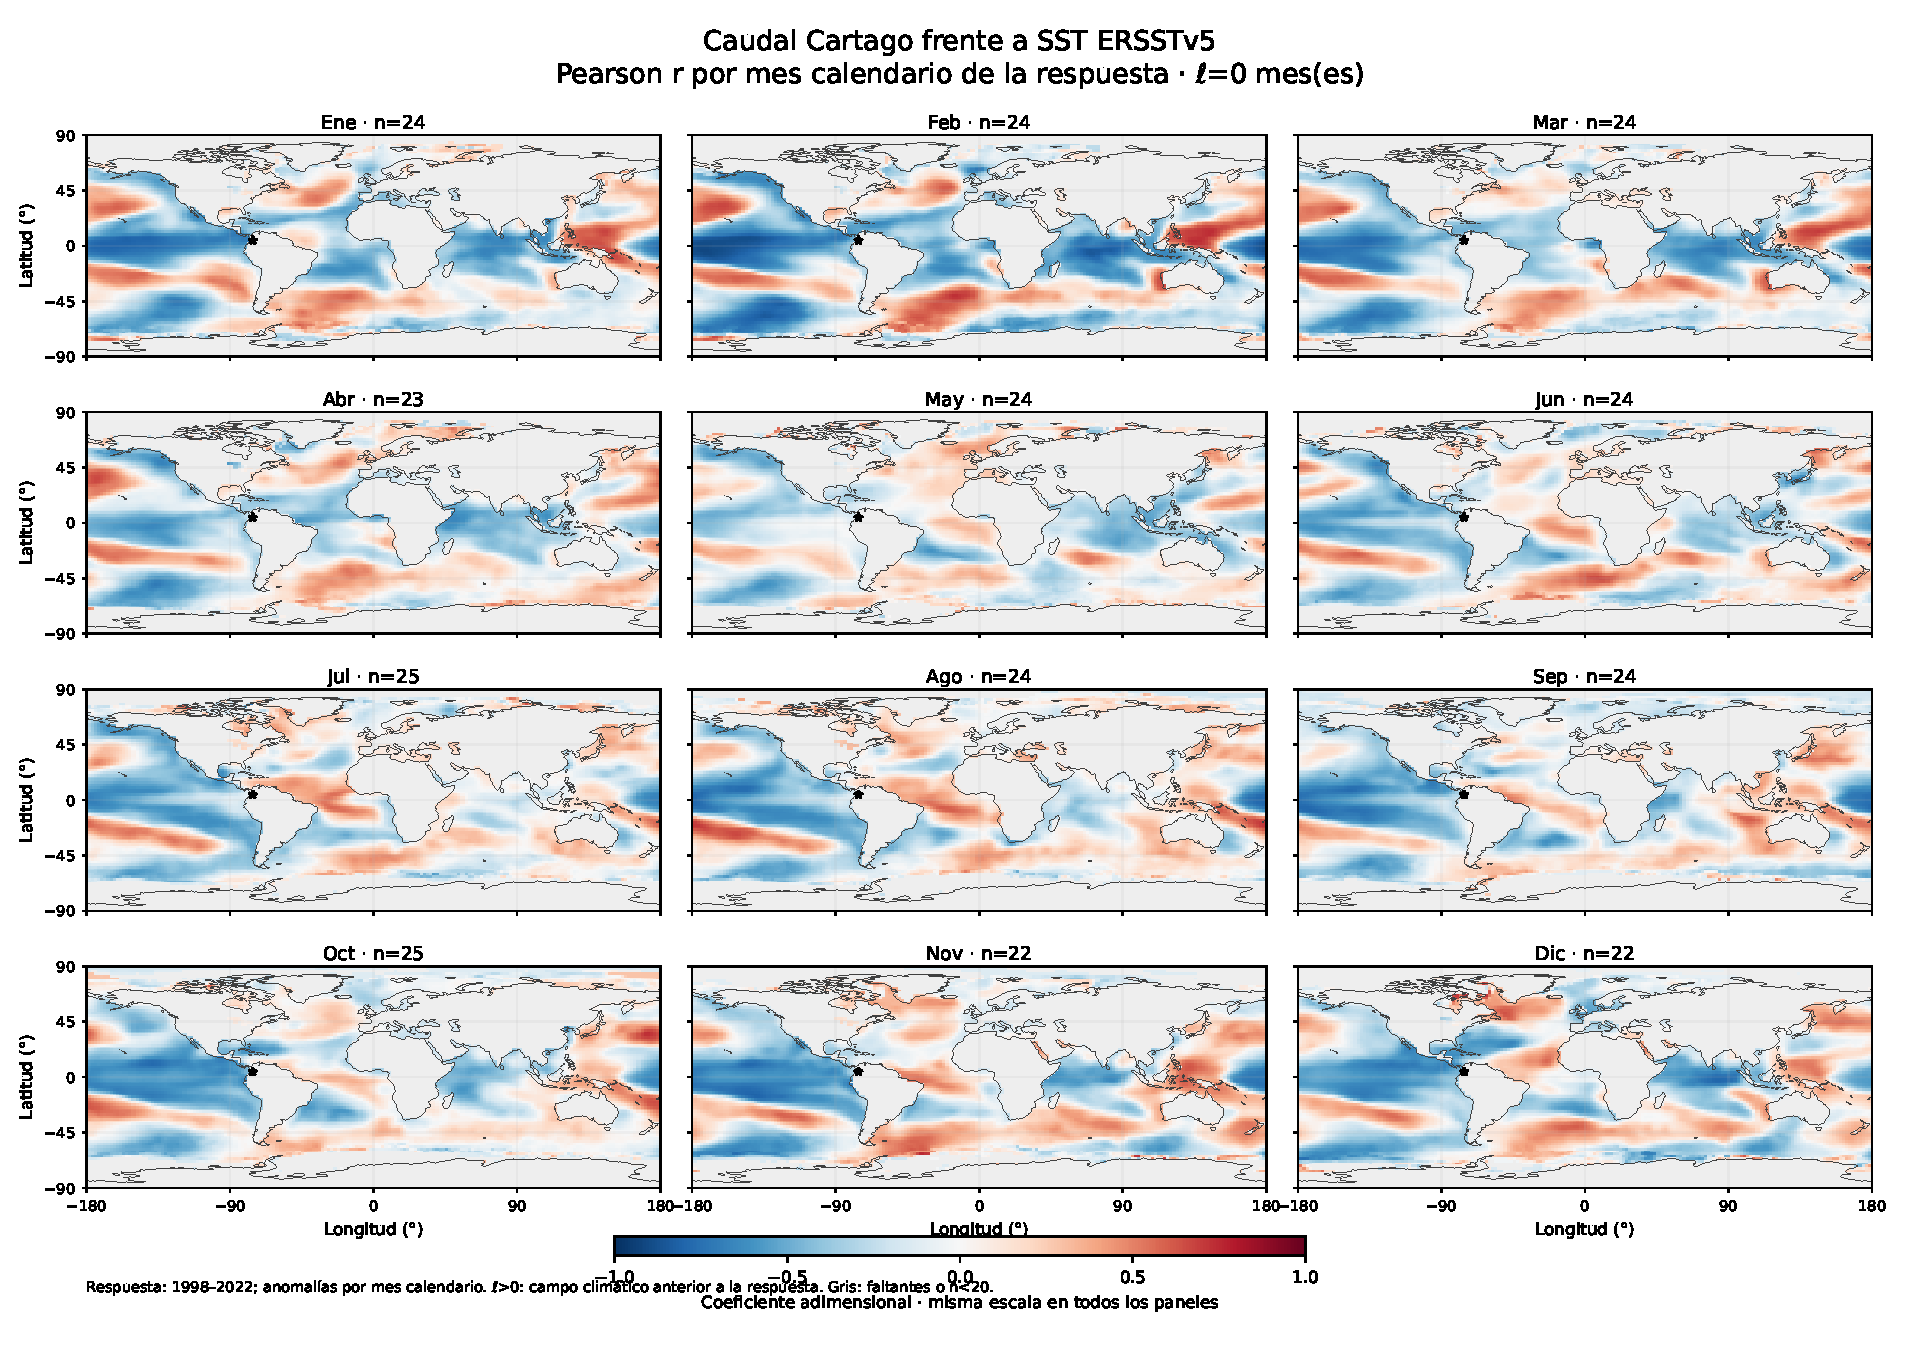
\includegraphics[width=\linewidth]{../apartado_5_2/Q_sst_l0_pearson.pdf}\caption{Doce correlaciones temporales por mes calendario; rezago 0 mes(es).}\end{figure}
\begin{figure}[p]\centering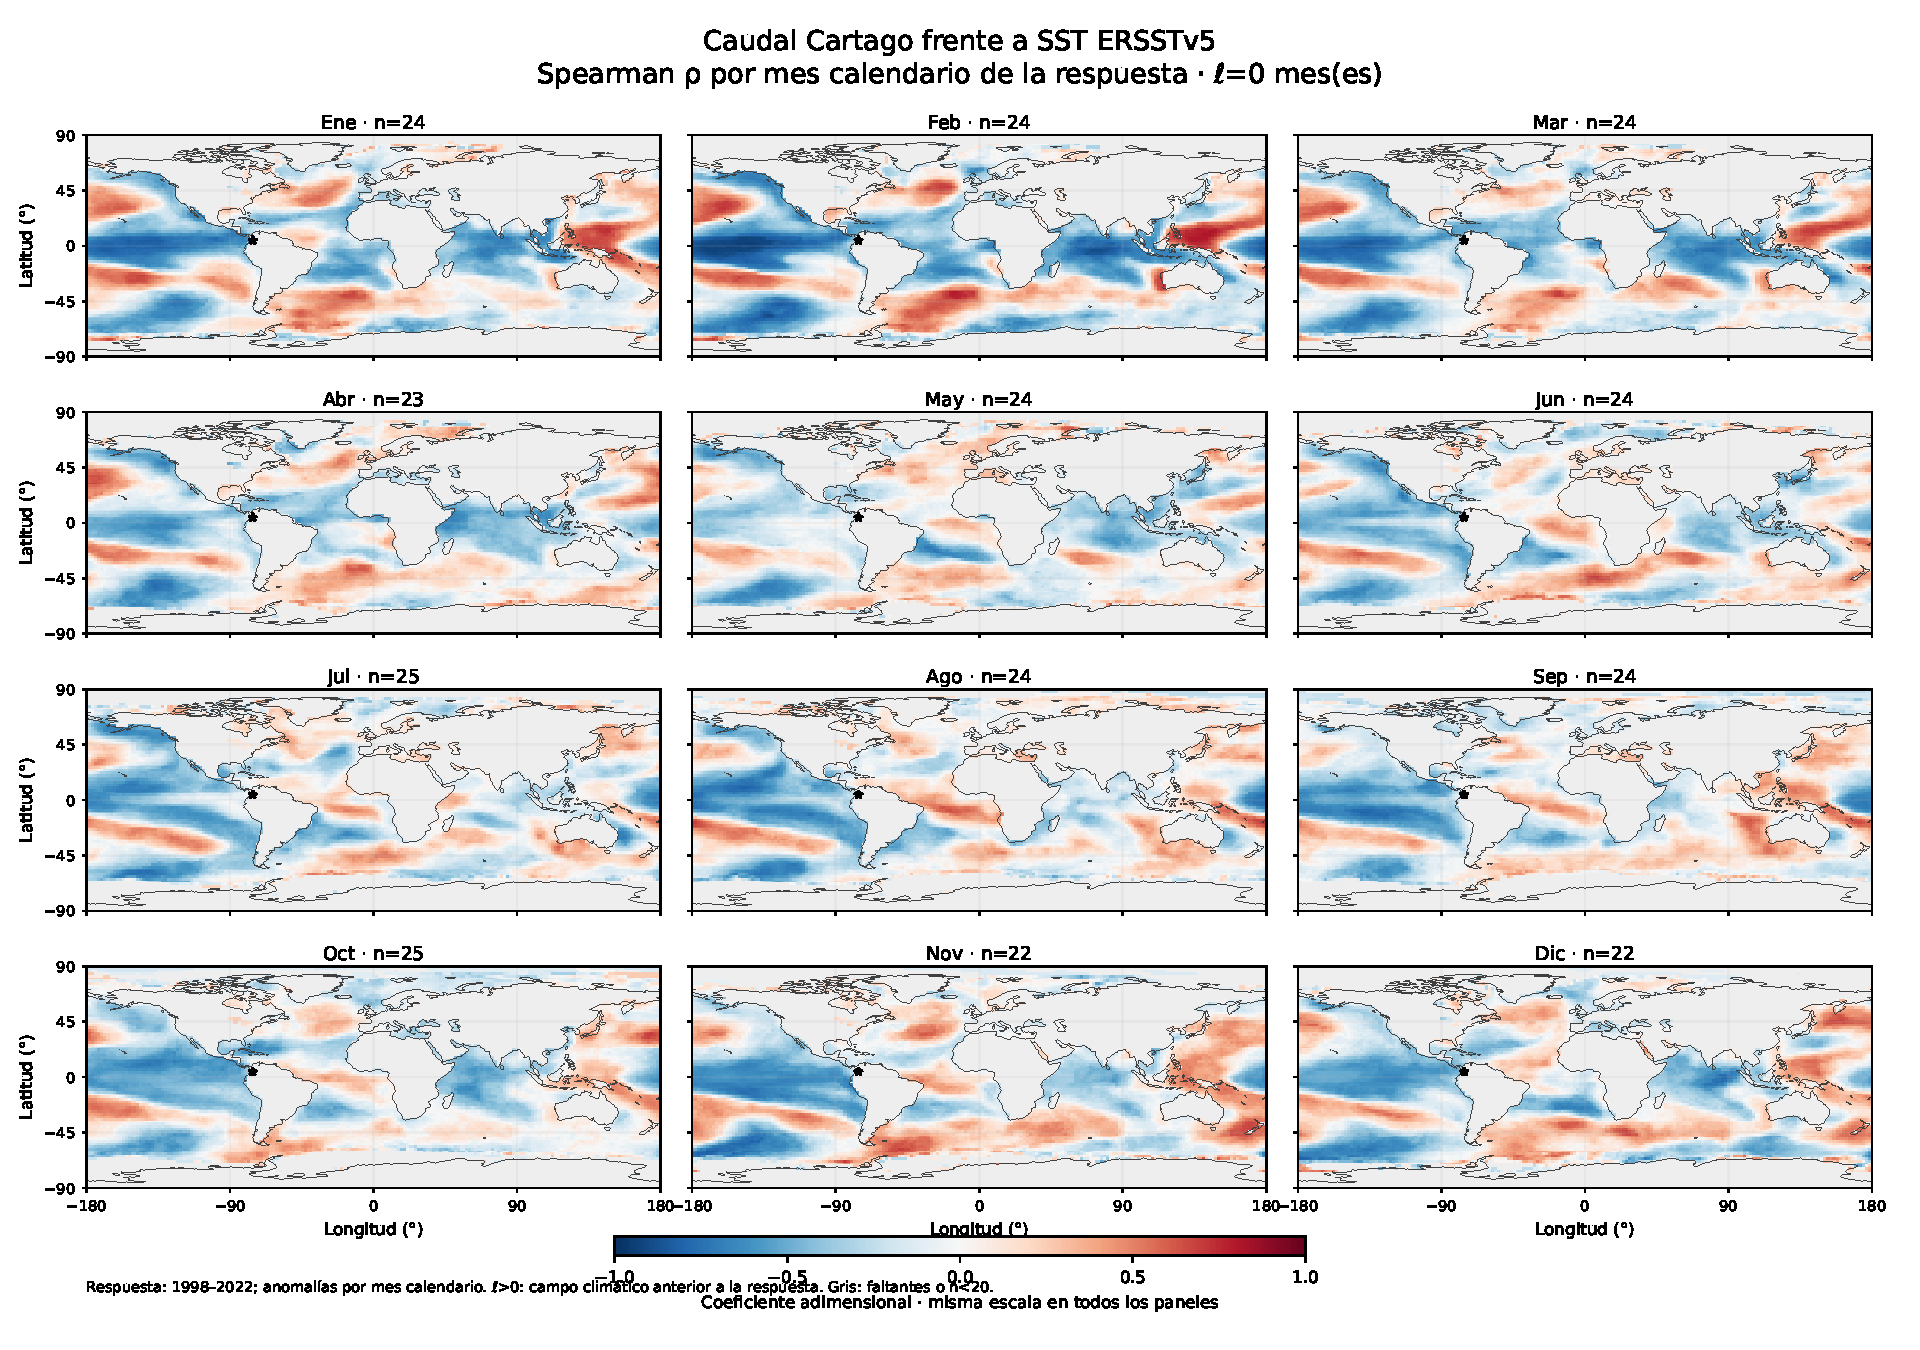
\includegraphics[width=\linewidth]{../apartado_5_2/Q_sst_l0_spearman.pdf}\caption{Doce correlaciones temporales por mes calendario; rezago 0 mes(es).}\end{figure}
\begin{figure}[p]\centering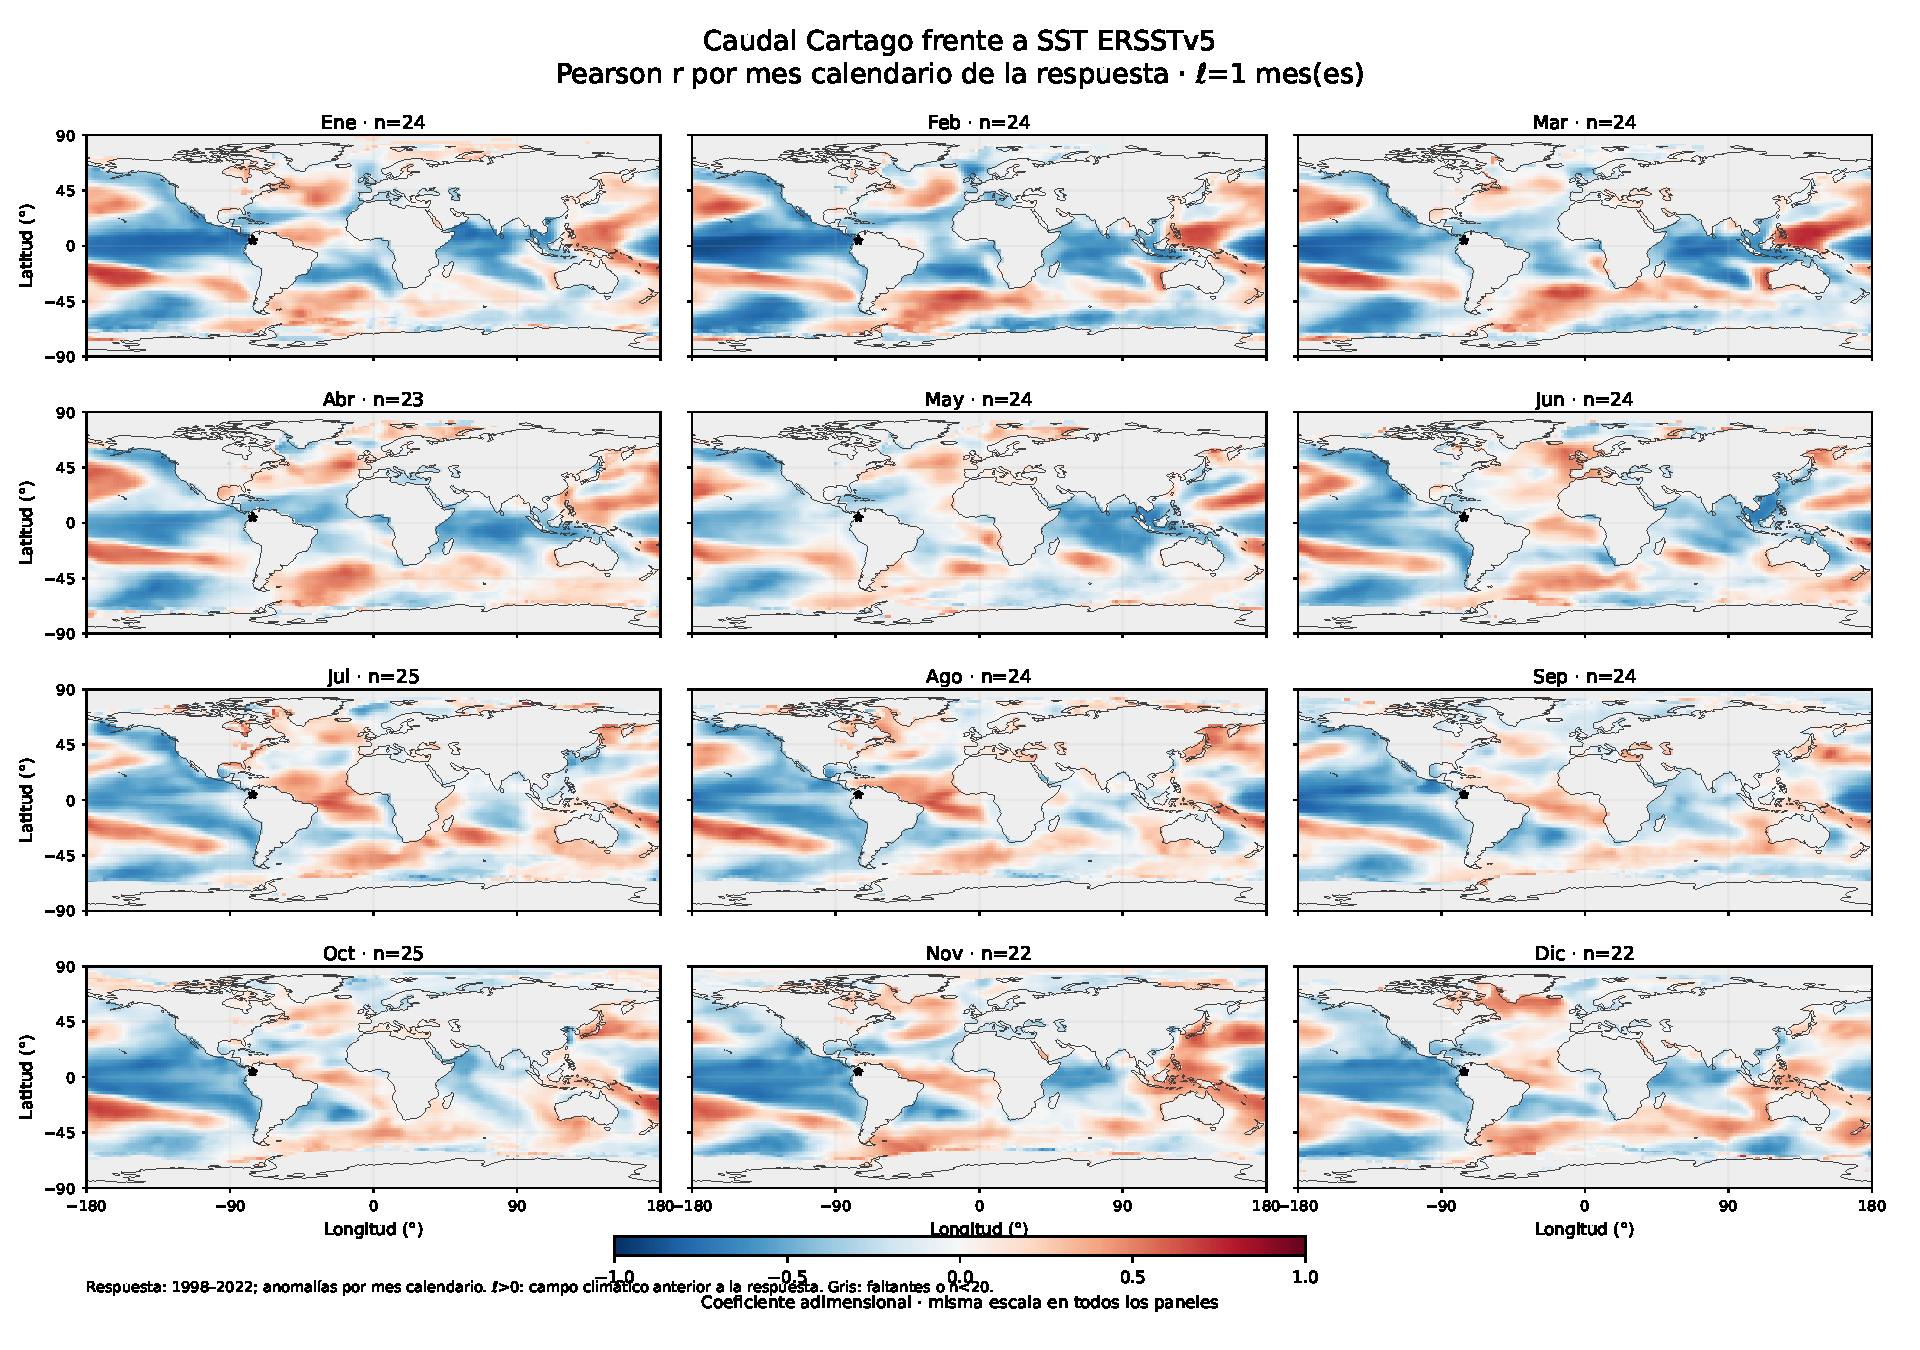
\includegraphics[width=\linewidth]{../apartado_5_2/Q_sst_l1_pearson.pdf}\caption{Doce correlaciones temporales por mes calendario; rezago 1 mes(es).}\end{figure}
\begin{figure}[p]\centering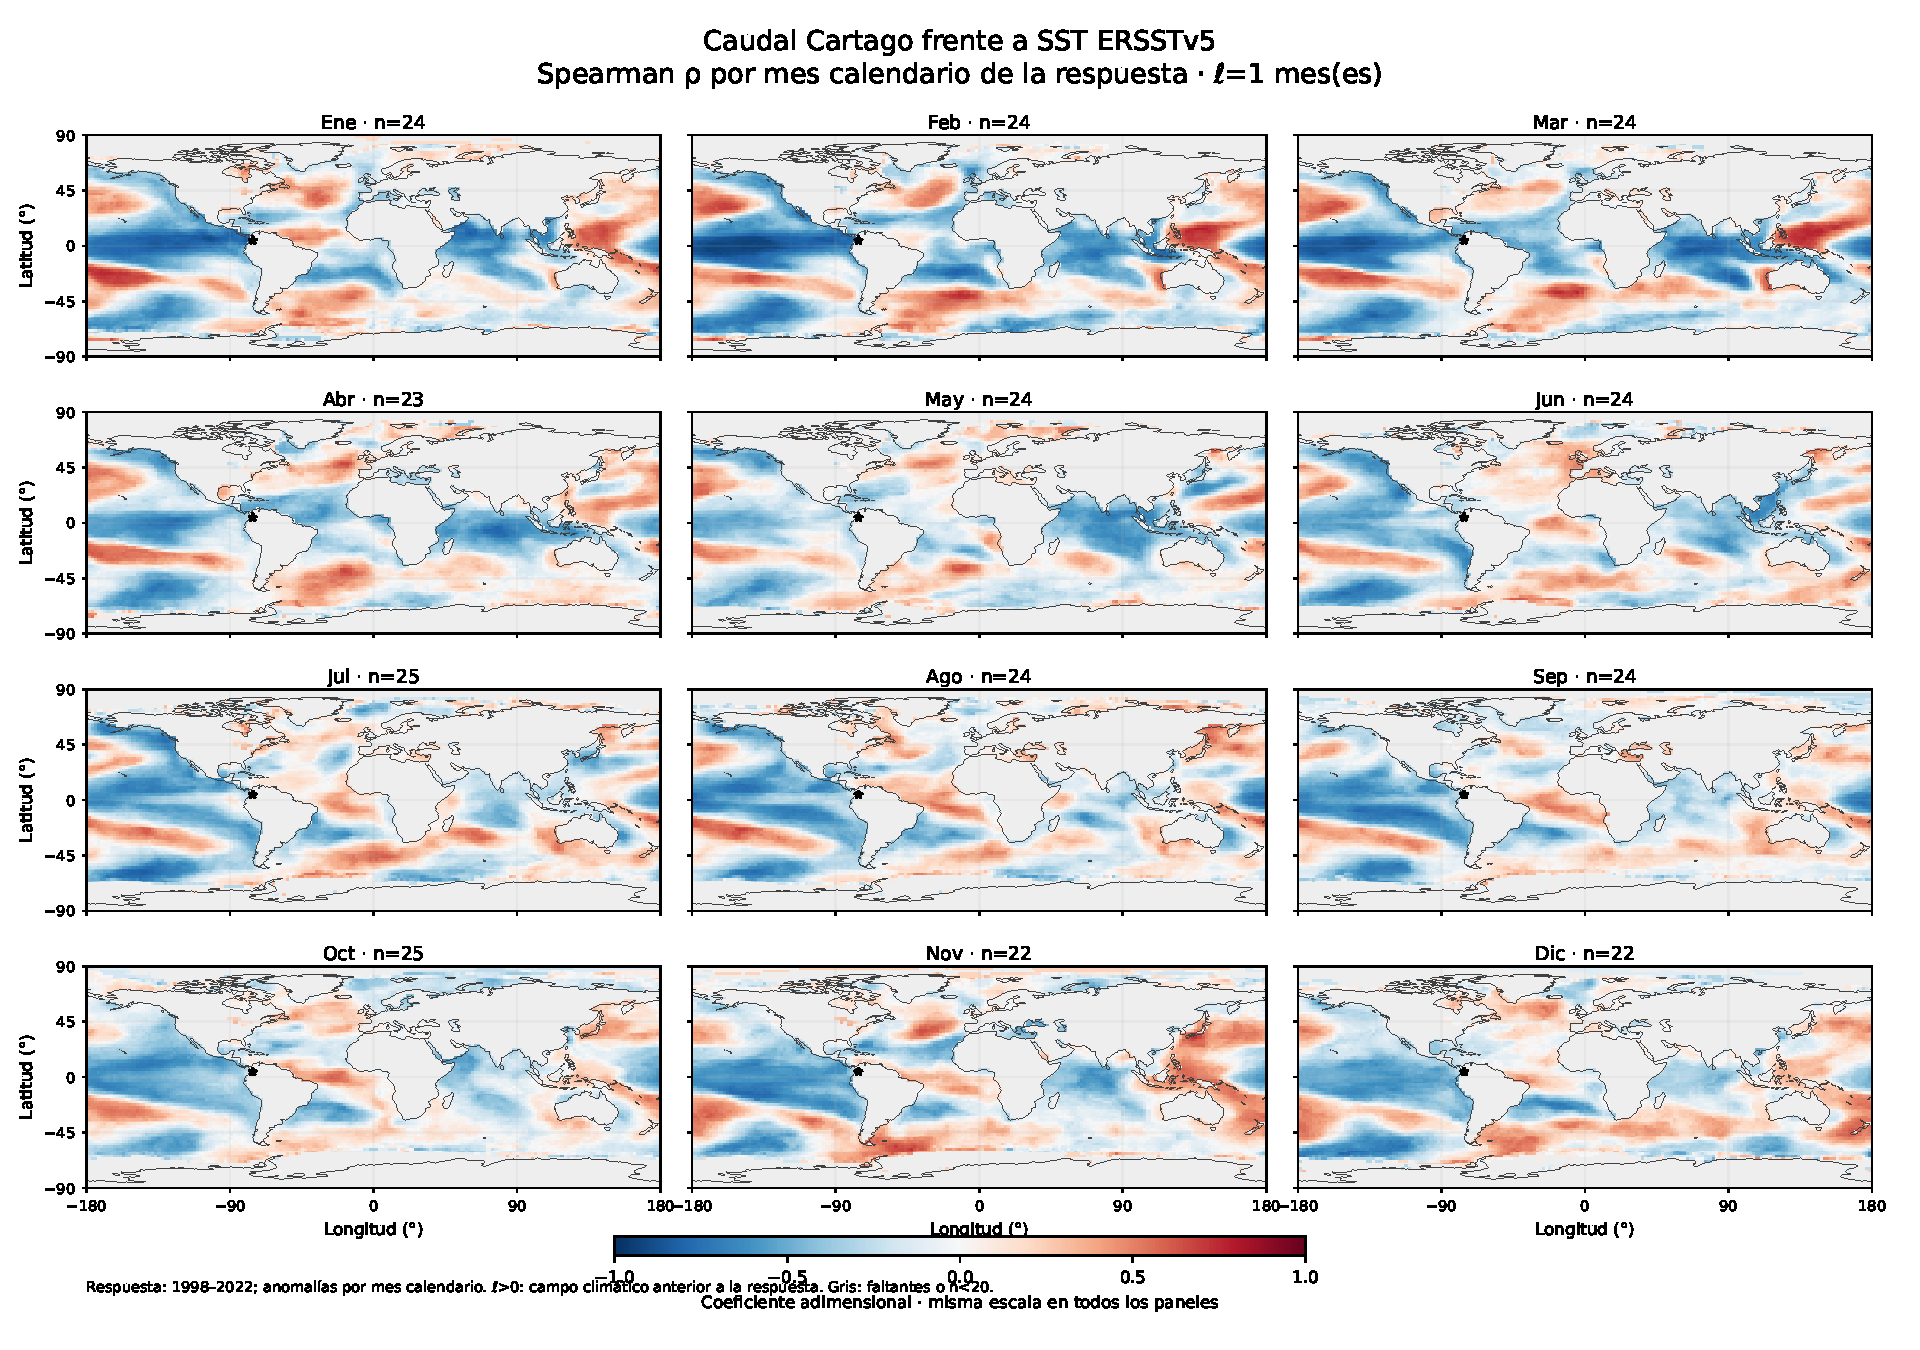
\includegraphics[width=\linewidth]{../apartado_5_2/Q_sst_l1_spearman.pdf}\caption{Doce correlaciones temporales por mes calendario; rezago 1 mes(es).}\end{figure}
\begin{figure}[p]\centering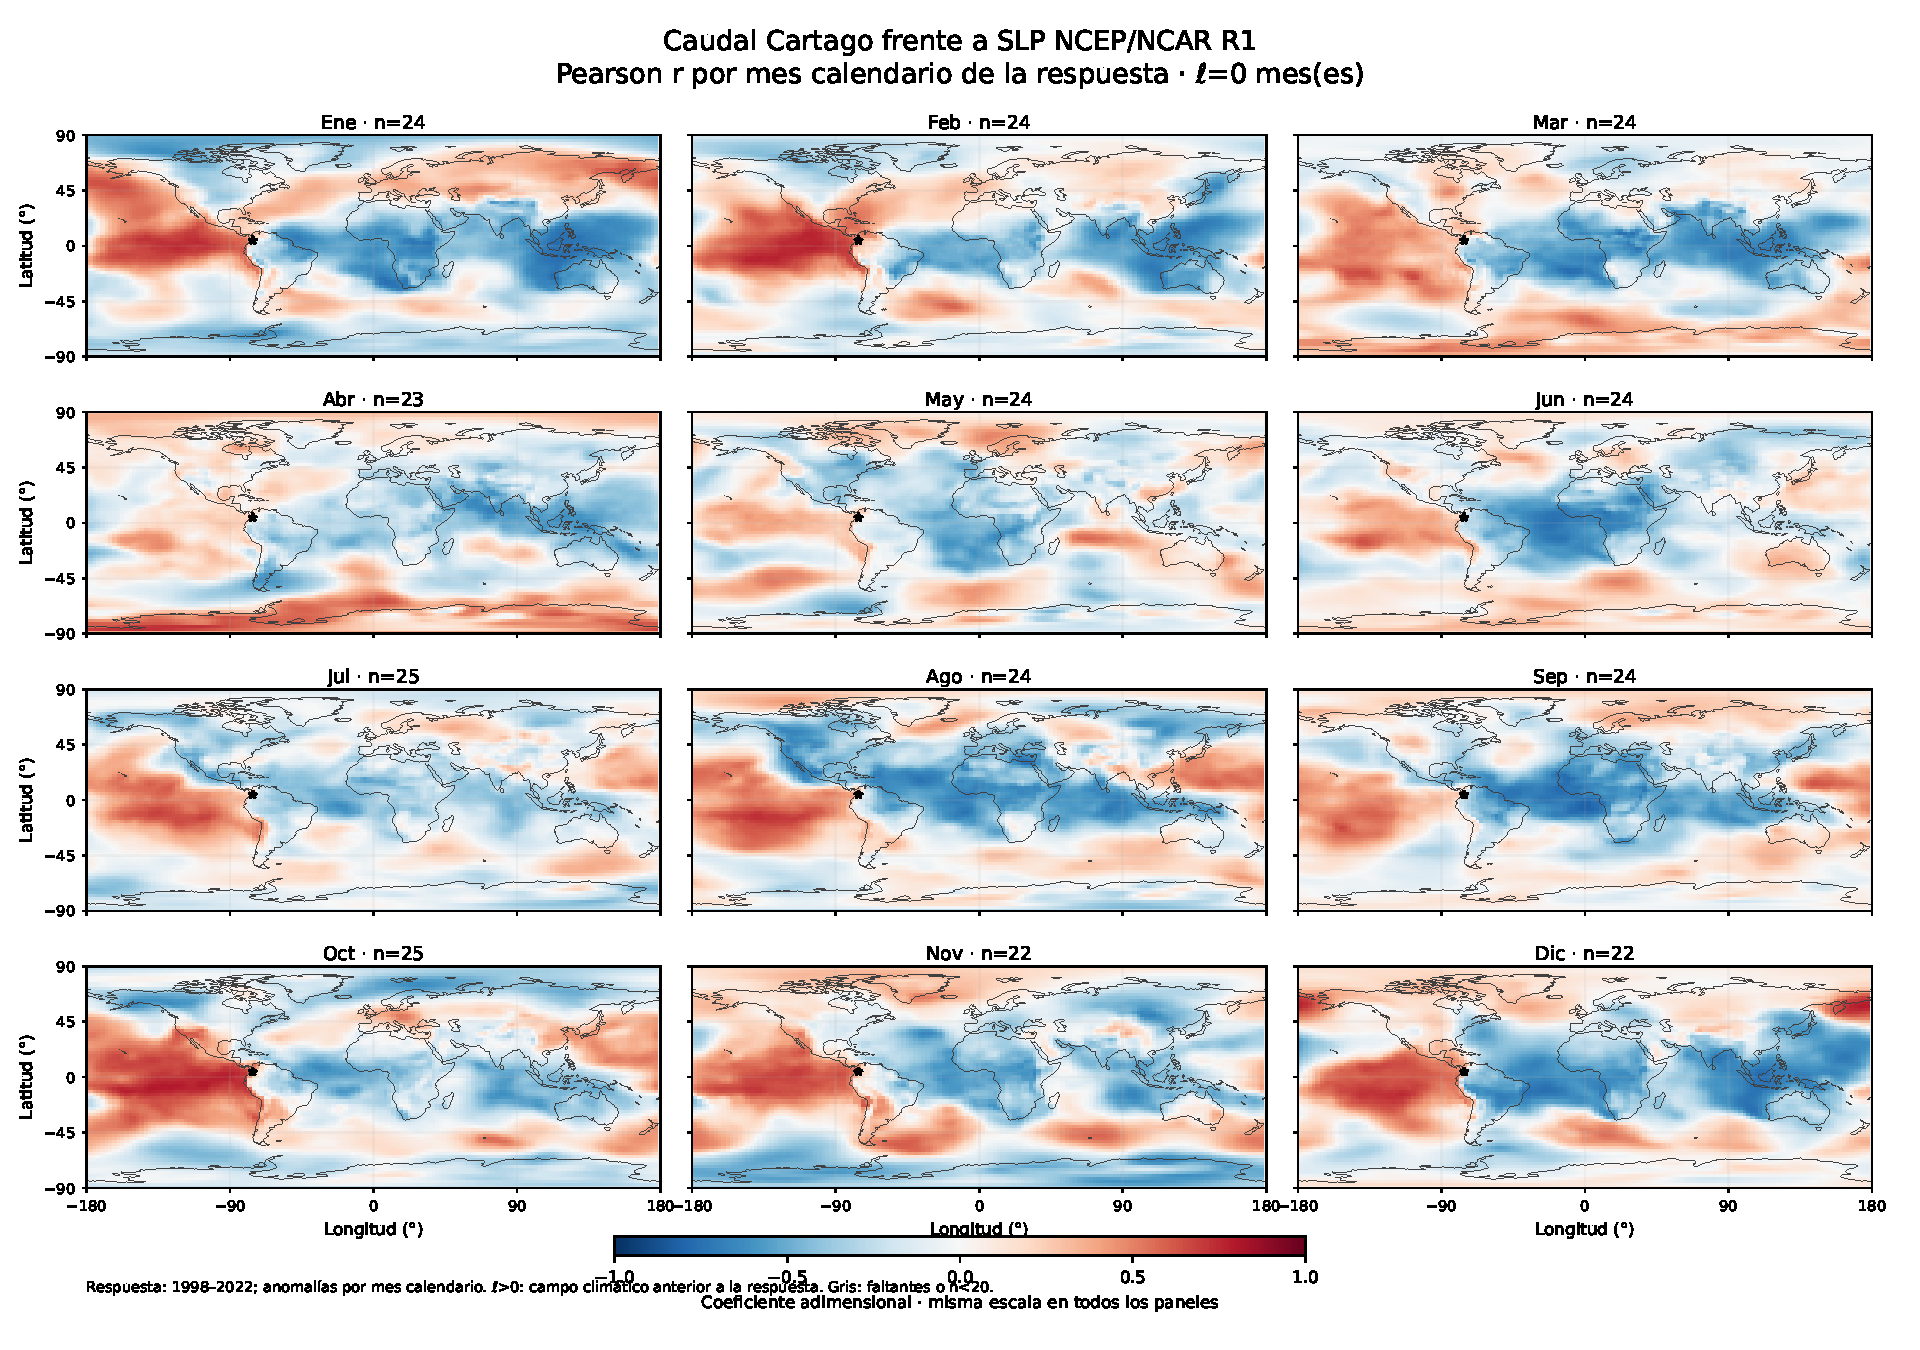
\includegraphics[width=\linewidth]{../apartado_5_2/Q_slp_l0_pearson.pdf}\caption{Doce correlaciones temporales por mes calendario; rezago 0 mes(es).}\end{figure}
\begin{figure}[p]\centering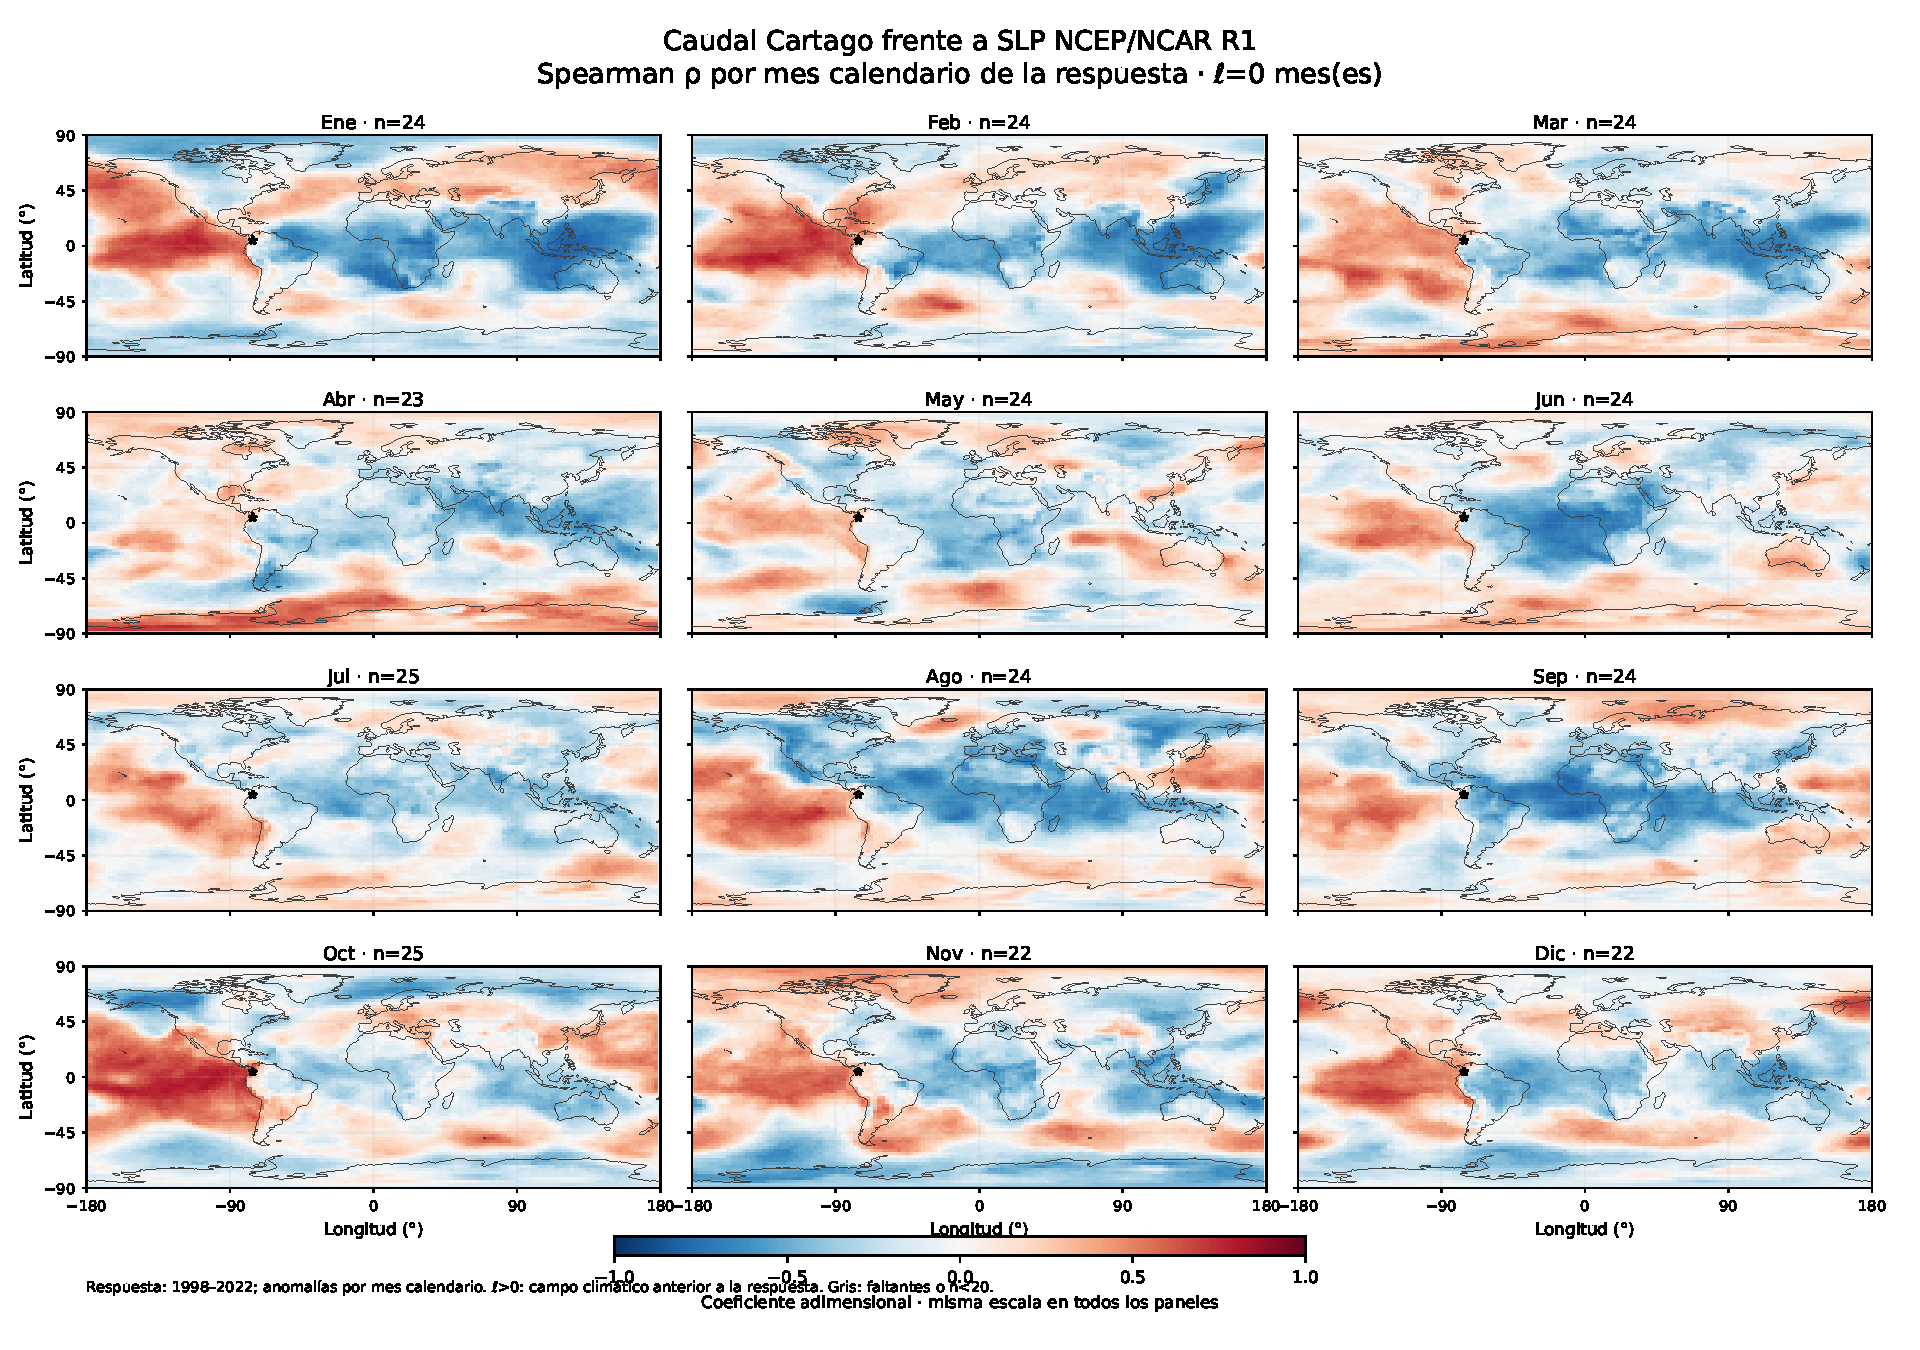
\includegraphics[width=\linewidth]{../apartado_5_2/Q_slp_l0_spearman.pdf}\caption{Doce correlaciones temporales por mes calendario; rezago 0 mes(es).}\end{figure}
\begin{figure}[p]\centering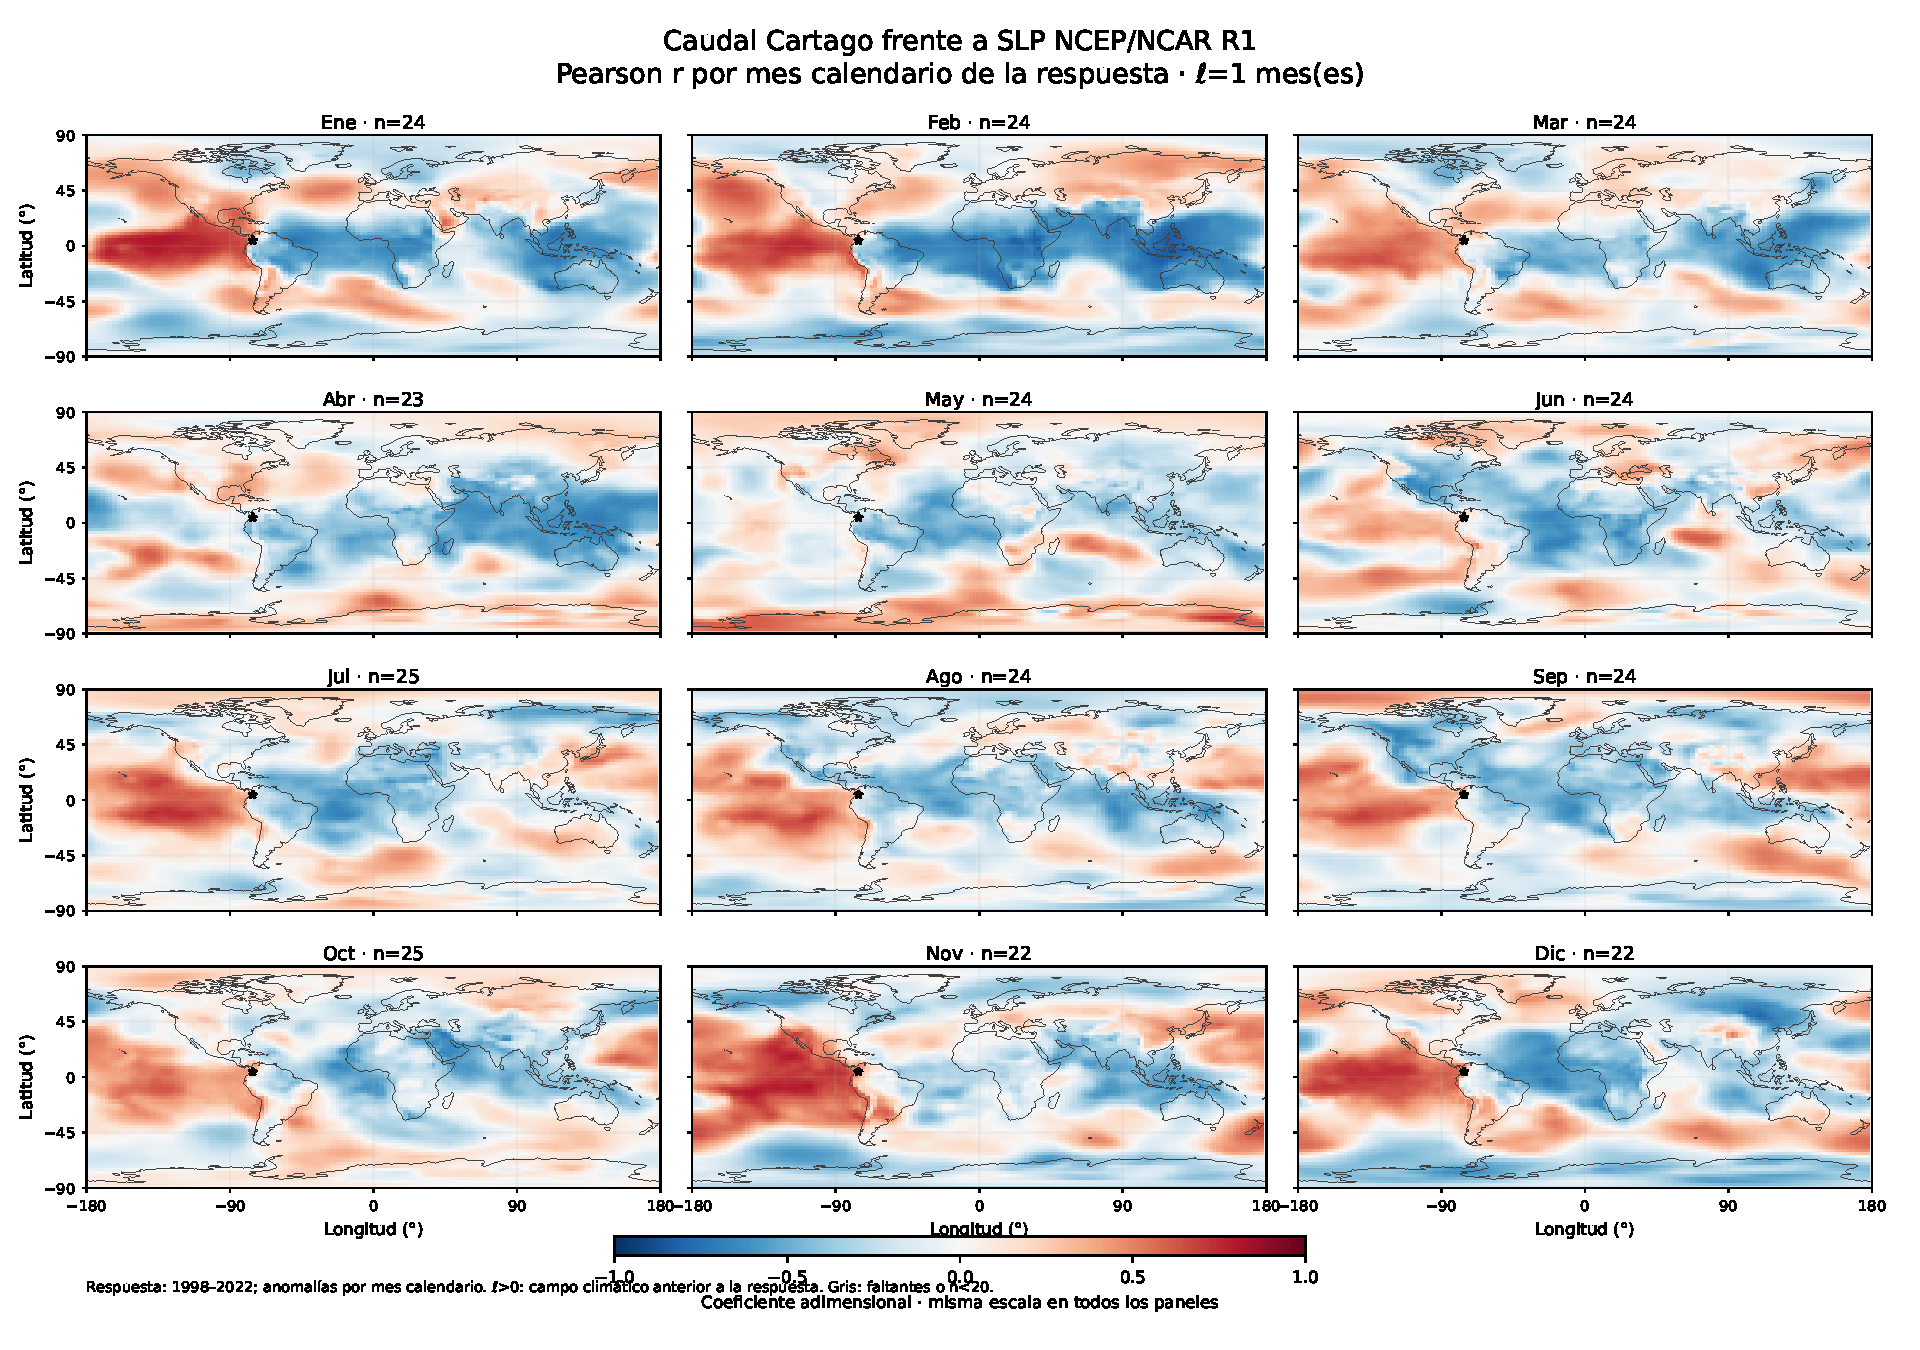
\includegraphics[width=\linewidth]{../apartado_5_2/Q_slp_l1_pearson.pdf}\caption{Doce correlaciones temporales por mes calendario; rezago 1 mes(es).}\end{figure}
\begin{figure}[p]\centering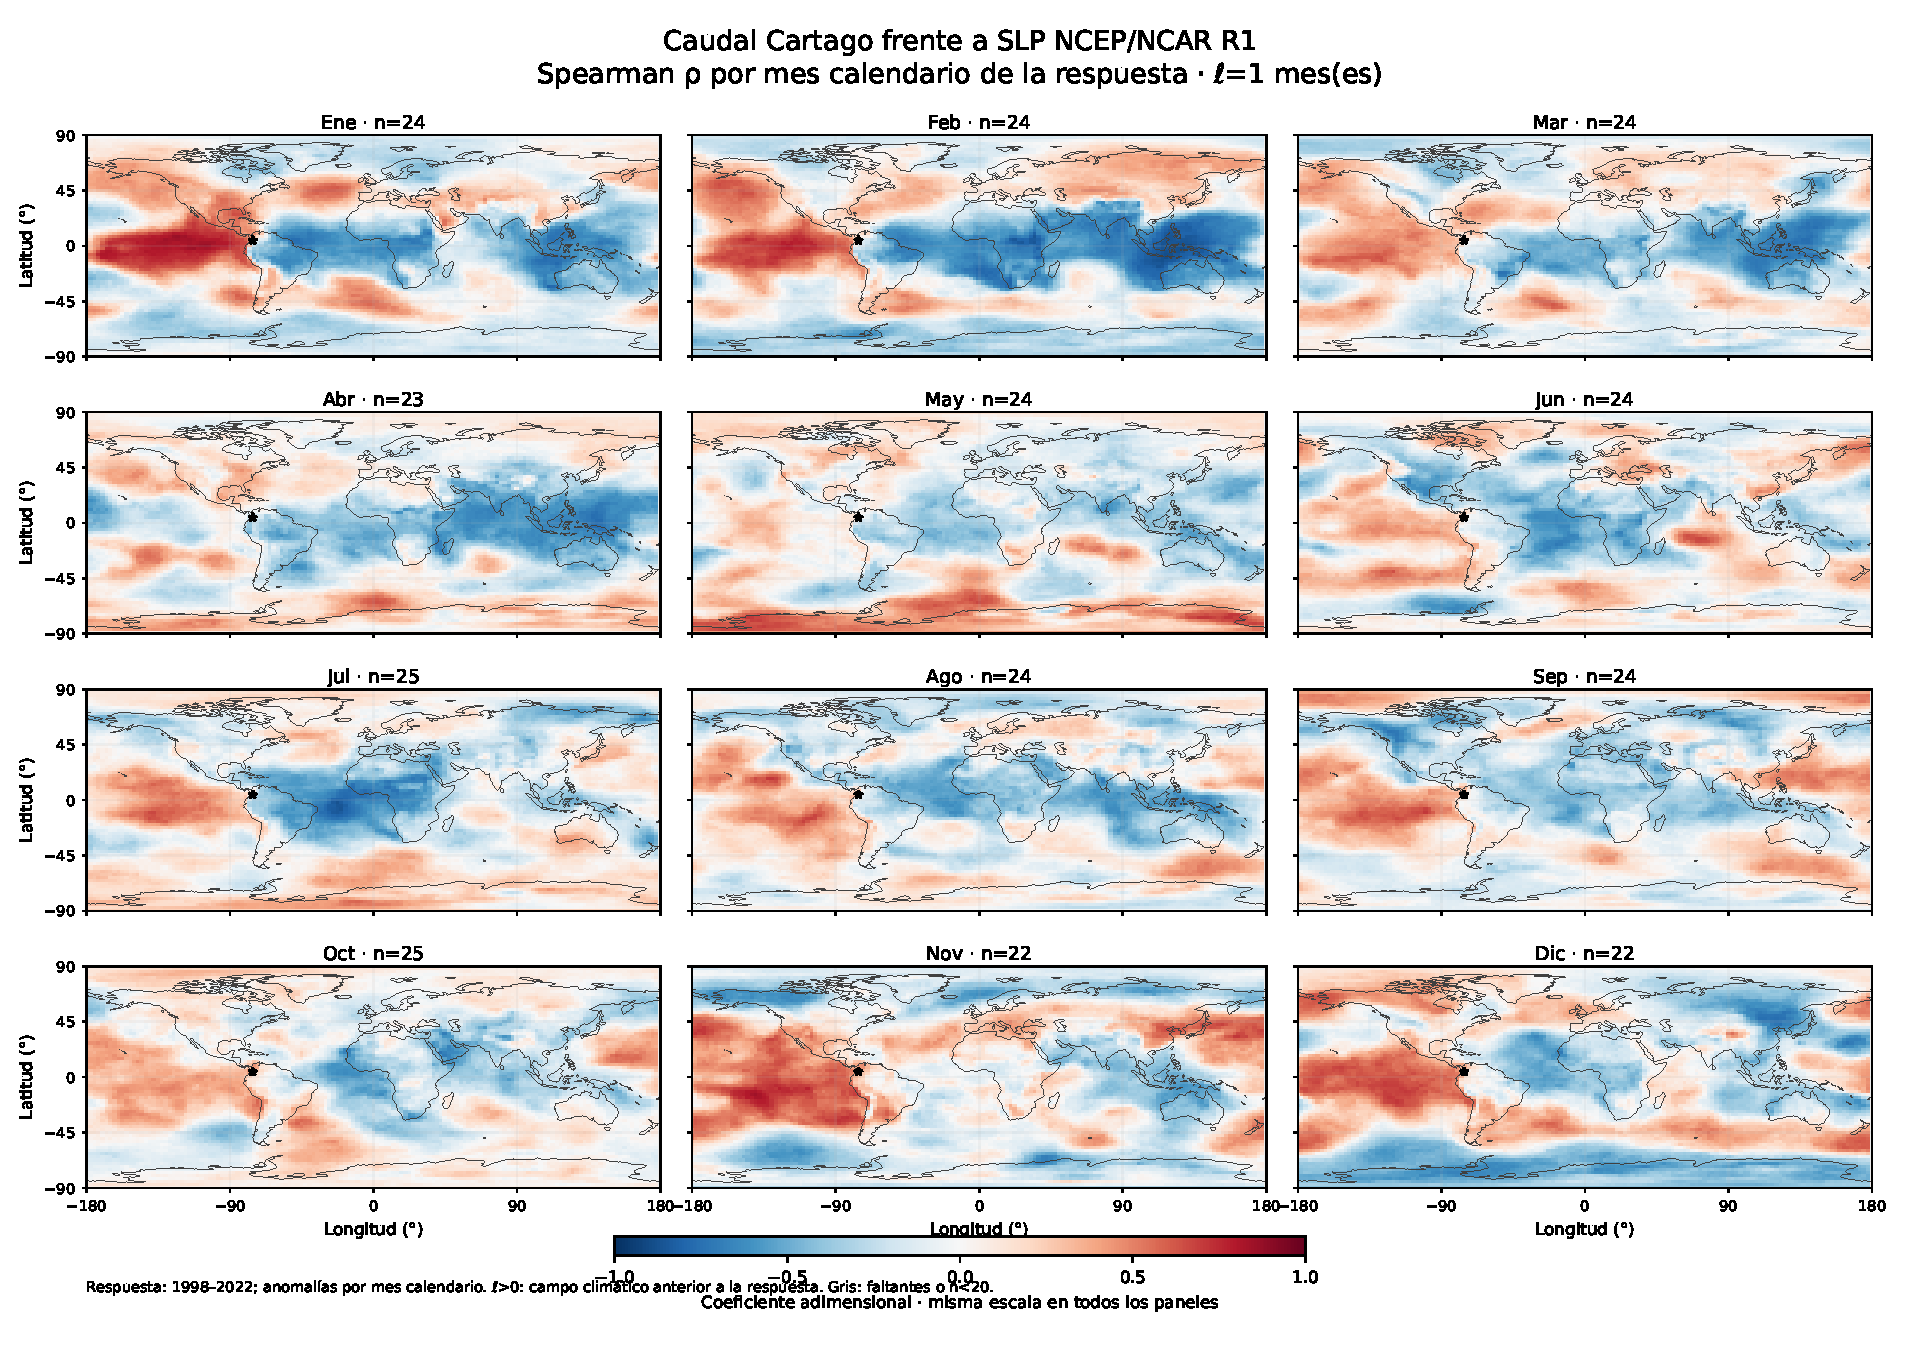
\includegraphics[width=\linewidth]{../apartado_5_2/Q_slp_l1_spearman.pdf}\caption{Doce correlaciones temporales por mes calendario; rezago 1 mes(es).}\end{figure}
\begin{figure}[p]\centering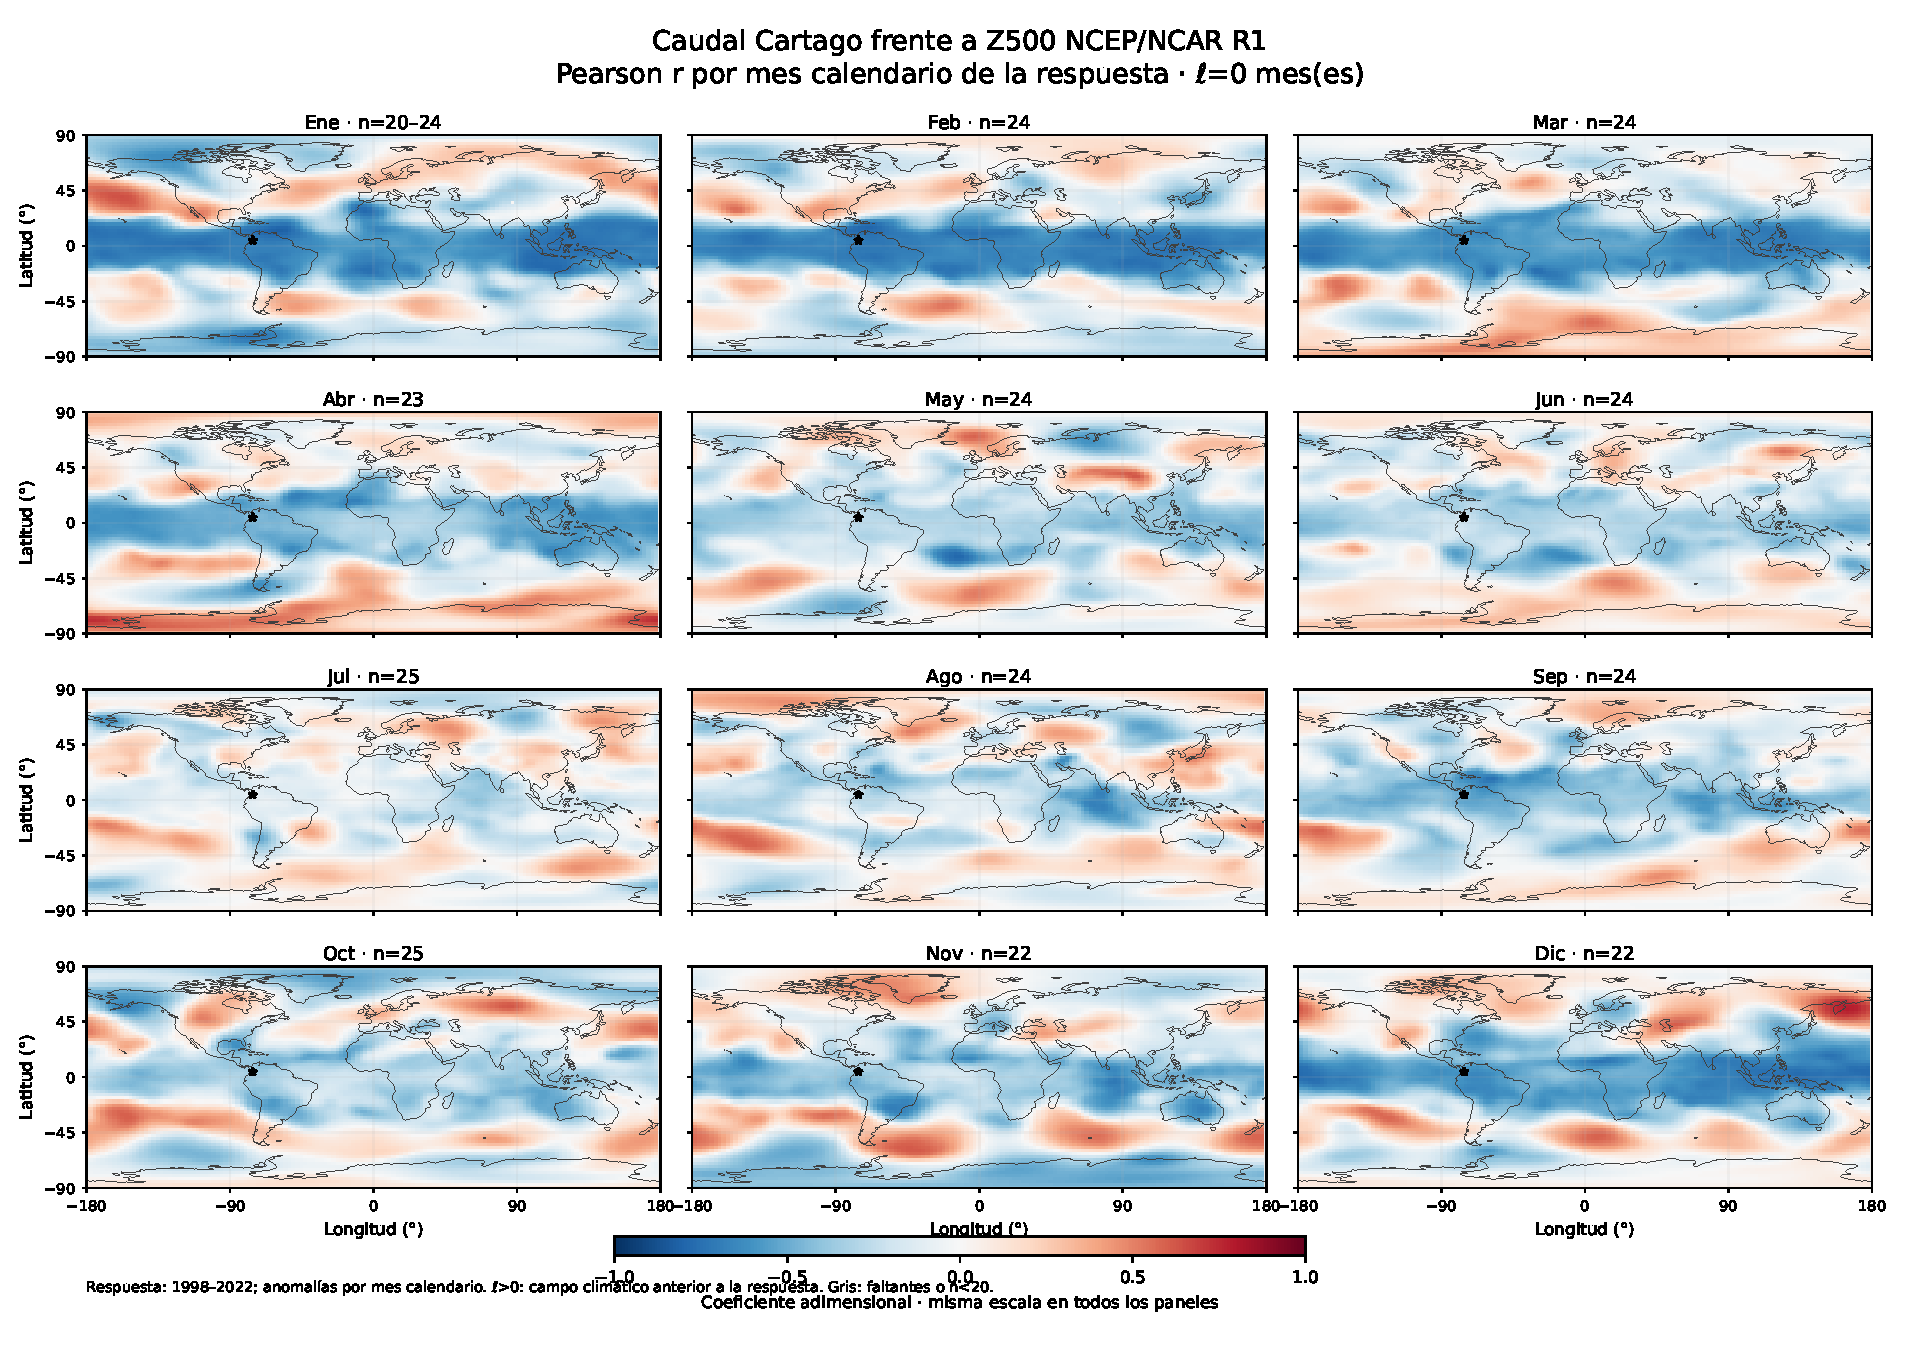
\includegraphics[width=\linewidth]{../apartado_5_2/Q_z500_l0_pearson.pdf}\caption{Doce correlaciones temporales por mes calendario; rezago 0 mes(es).}\end{figure}
\begin{figure}[p]\centering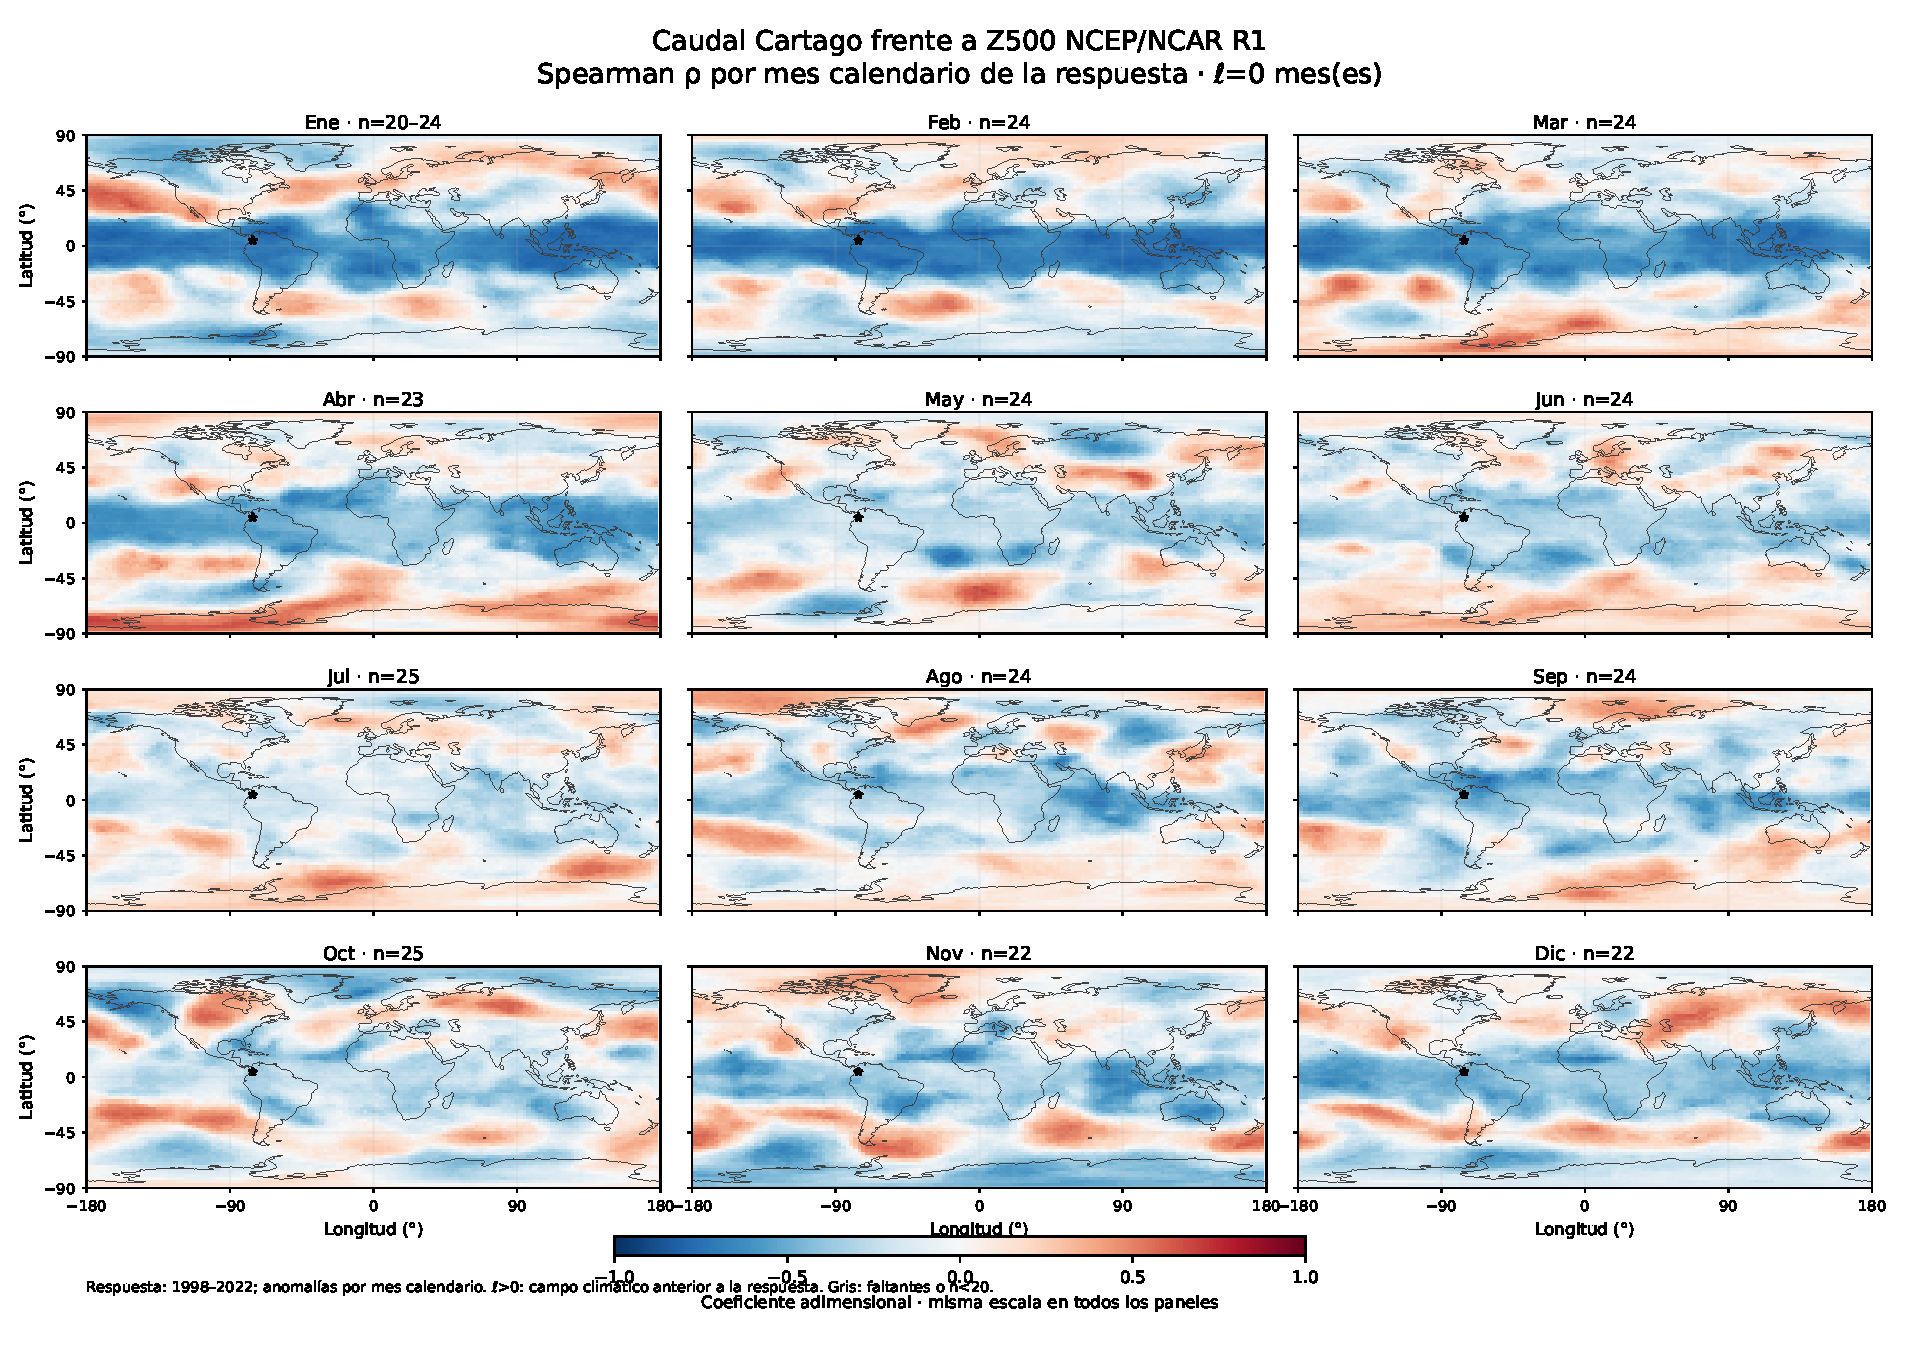
\includegraphics[width=\linewidth]{../apartado_5_2/Q_z500_l0_spearman.pdf}\caption{Doce correlaciones temporales por mes calendario; rezago 0 mes(es).}\end{figure}
\begin{figure}[p]\centering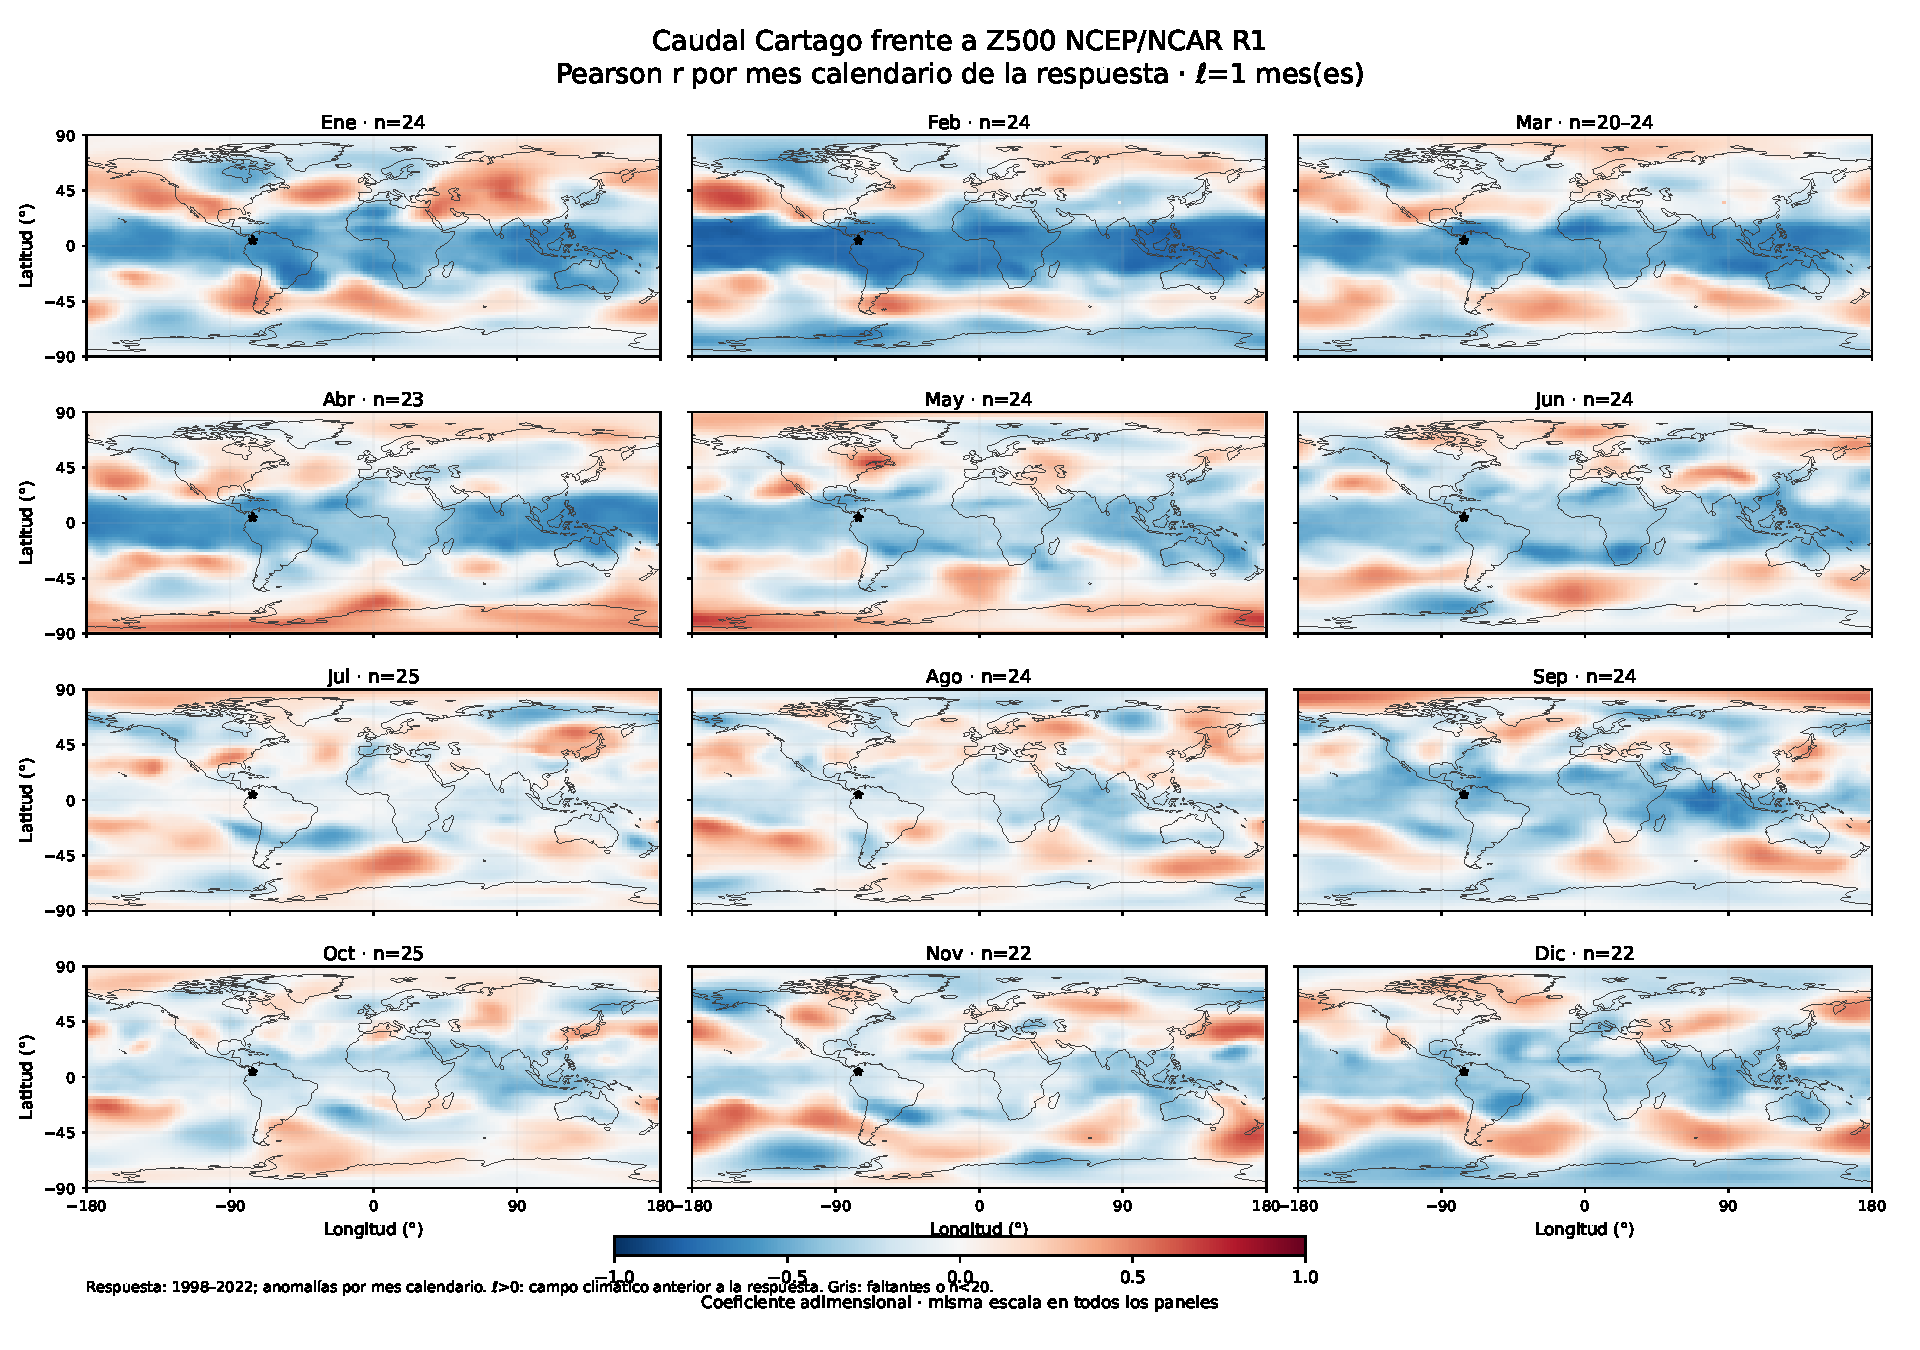
\includegraphics[width=\linewidth]{../apartado_5_2/Q_z500_l1_pearson.pdf}\caption{Doce correlaciones temporales por mes calendario; rezago 1 mes(es).}\end{figure}
\begin{figure}[p]\centering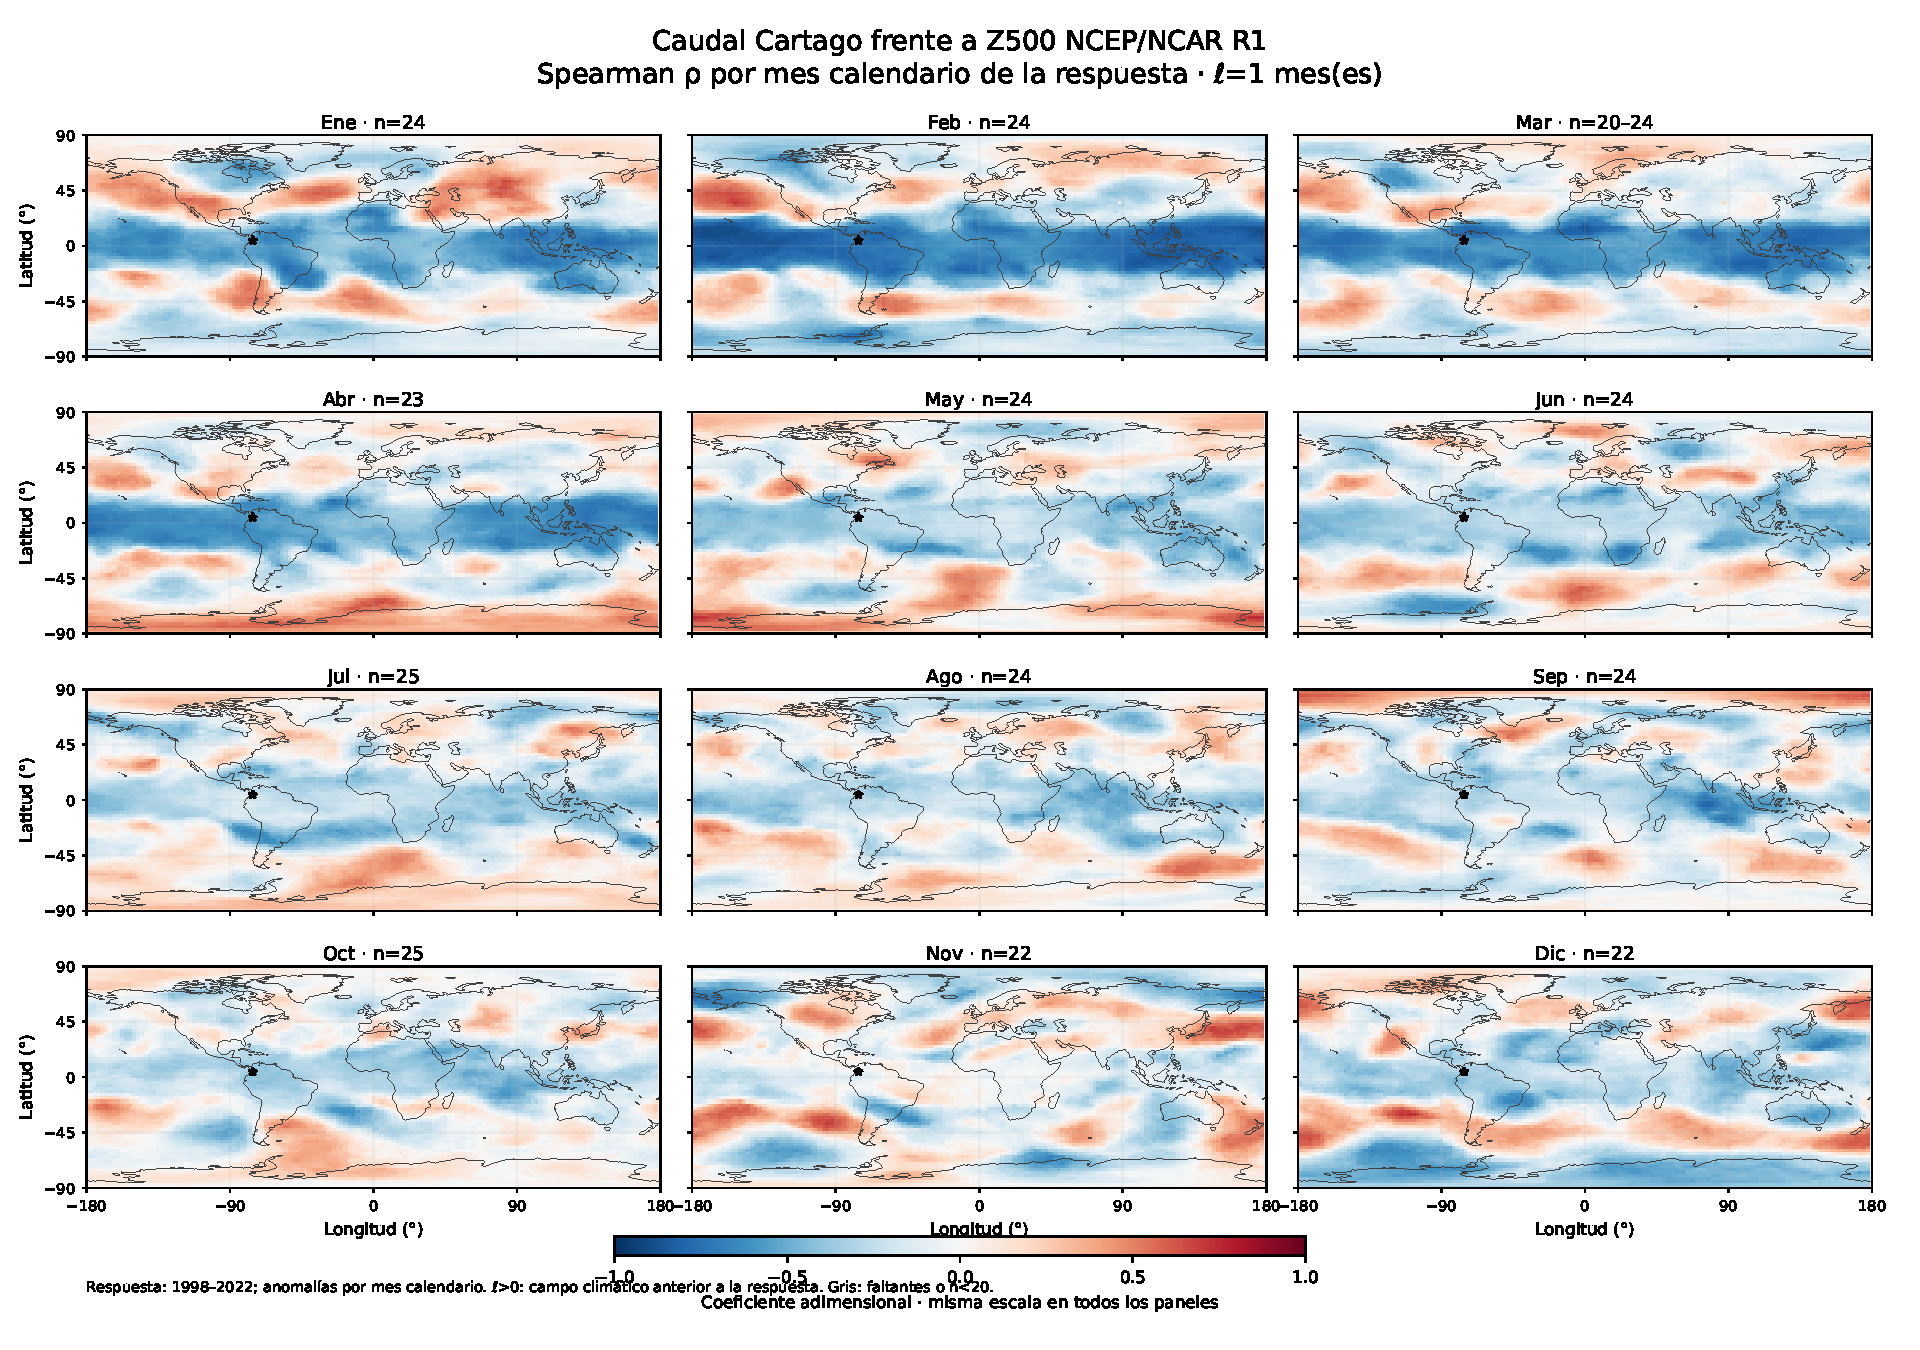
\includegraphics[width=\linewidth]{../apartado_5_2/Q_z500_l1_spearman.pdf}\caption{Doce correlaciones temporales por mes calendario; rezago 1 mes(es).}\end{figure}
\begin{figure}[p]\centering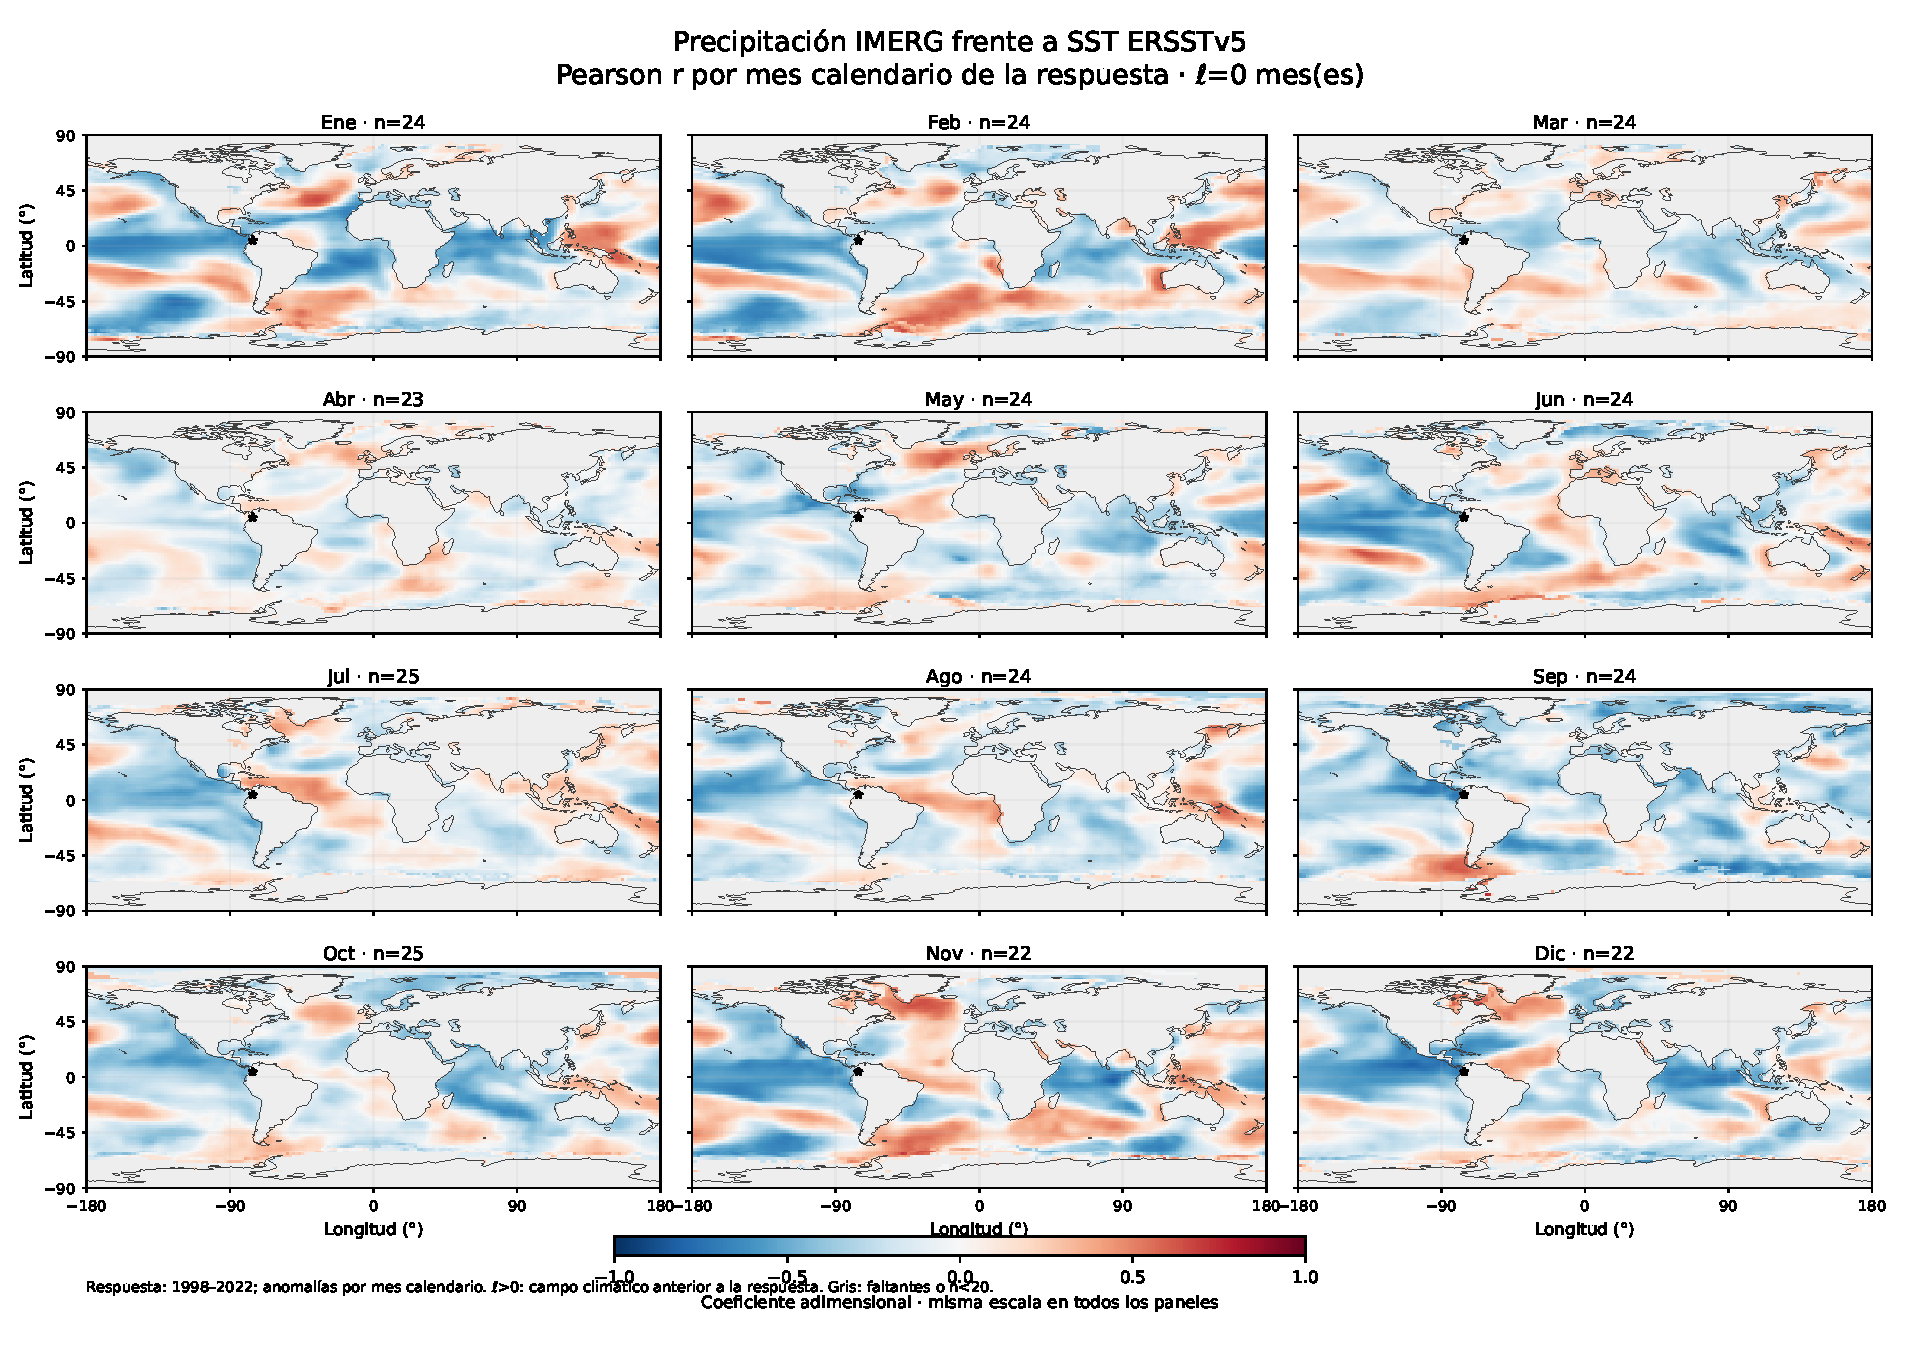
\includegraphics[width=\linewidth]{../apartado_5_2/IMERG_sst_l0_pearson.pdf}\caption{Doce correlaciones temporales por mes calendario; rezago 0 mes(es).}\end{figure}
\begin{figure}[p]\centering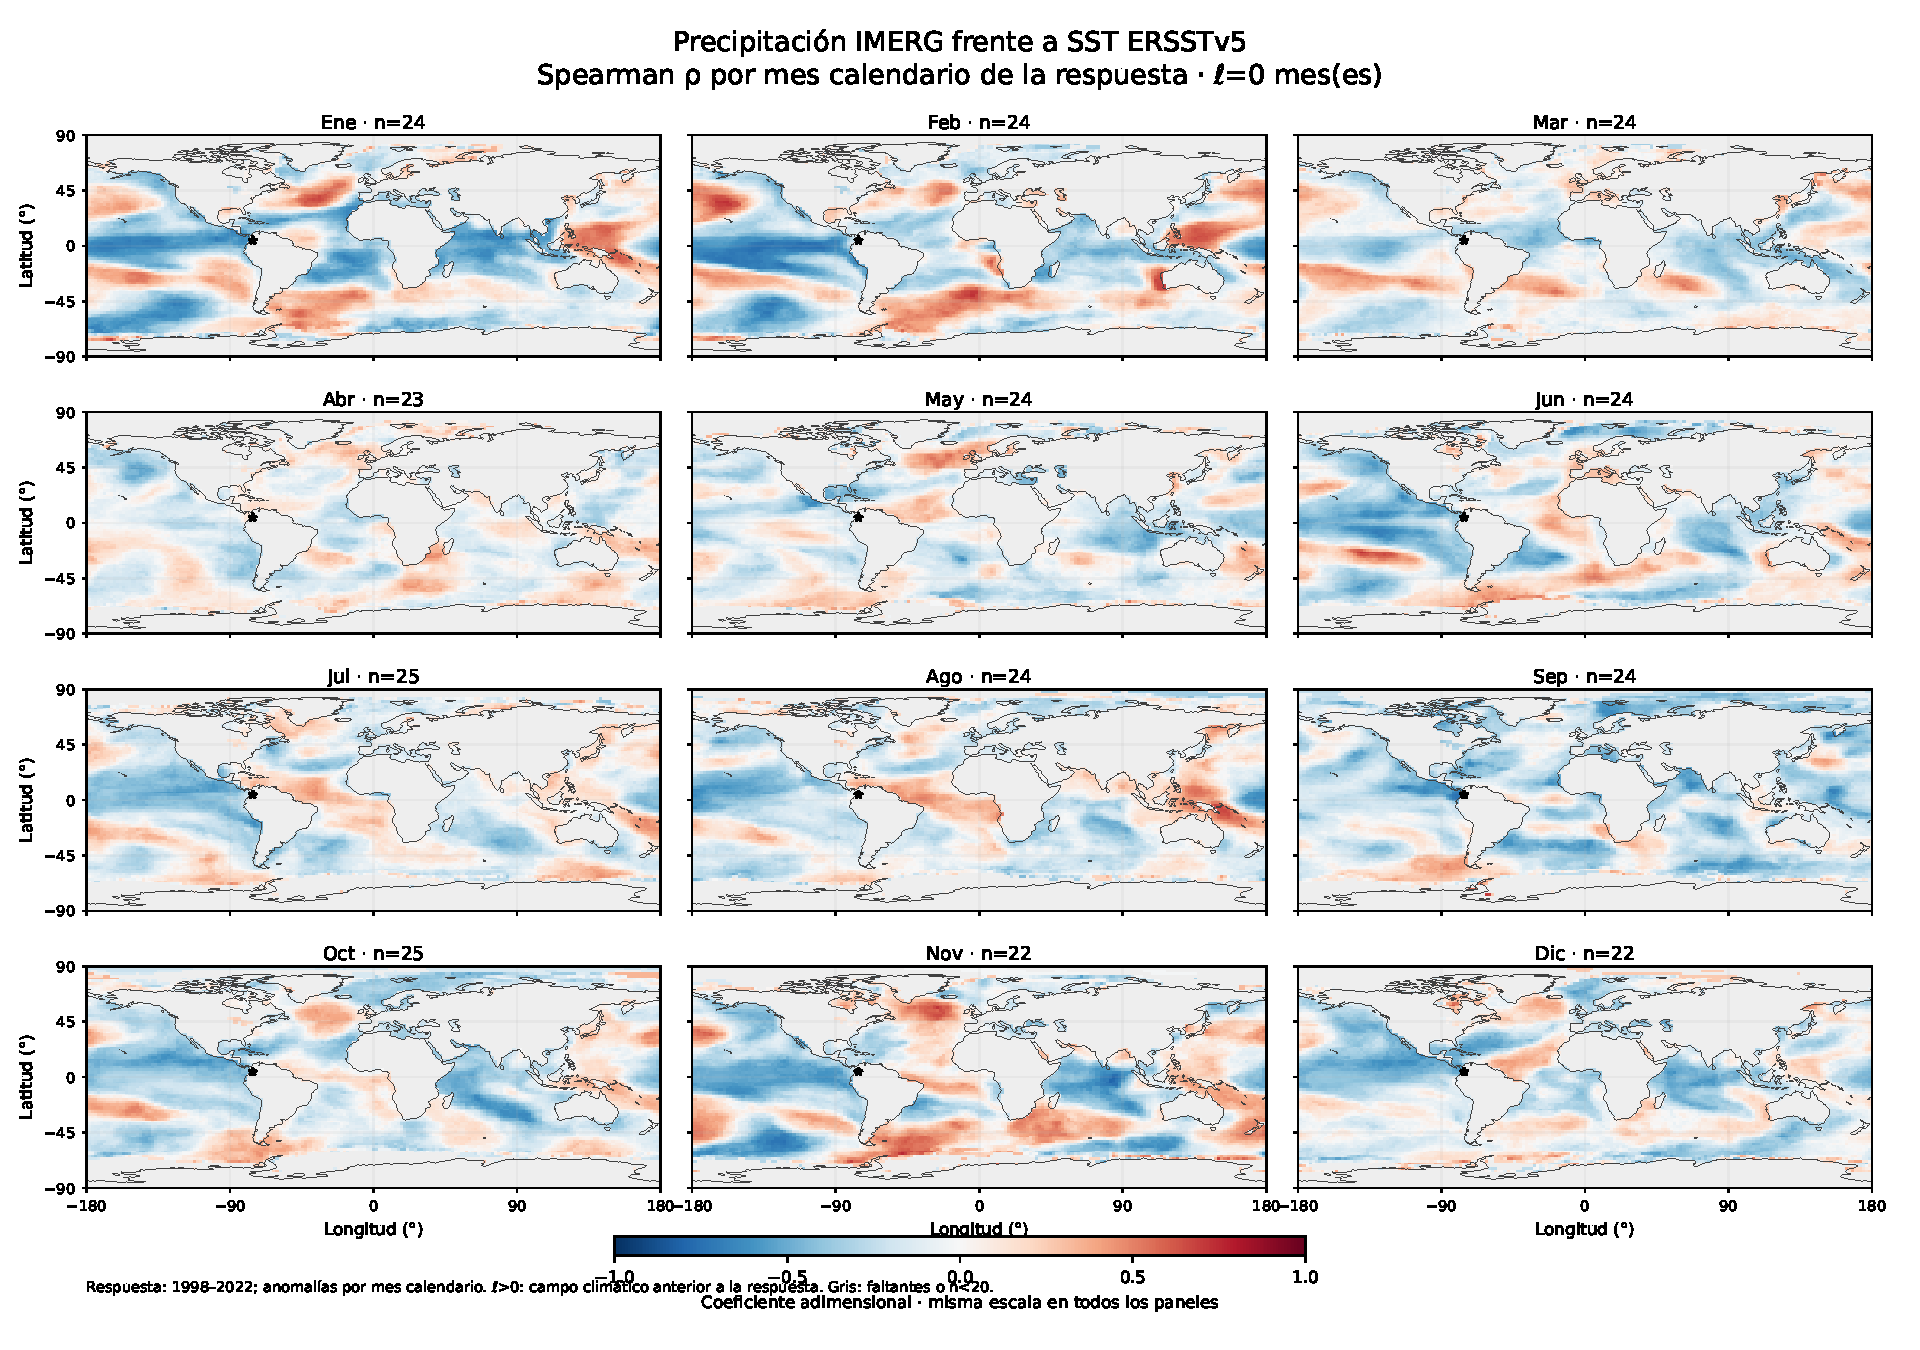
\includegraphics[width=\linewidth]{../apartado_5_2/IMERG_sst_l0_spearman.pdf}\caption{Doce correlaciones temporales por mes calendario; rezago 0 mes(es).}\end{figure}
\begin{figure}[p]\centering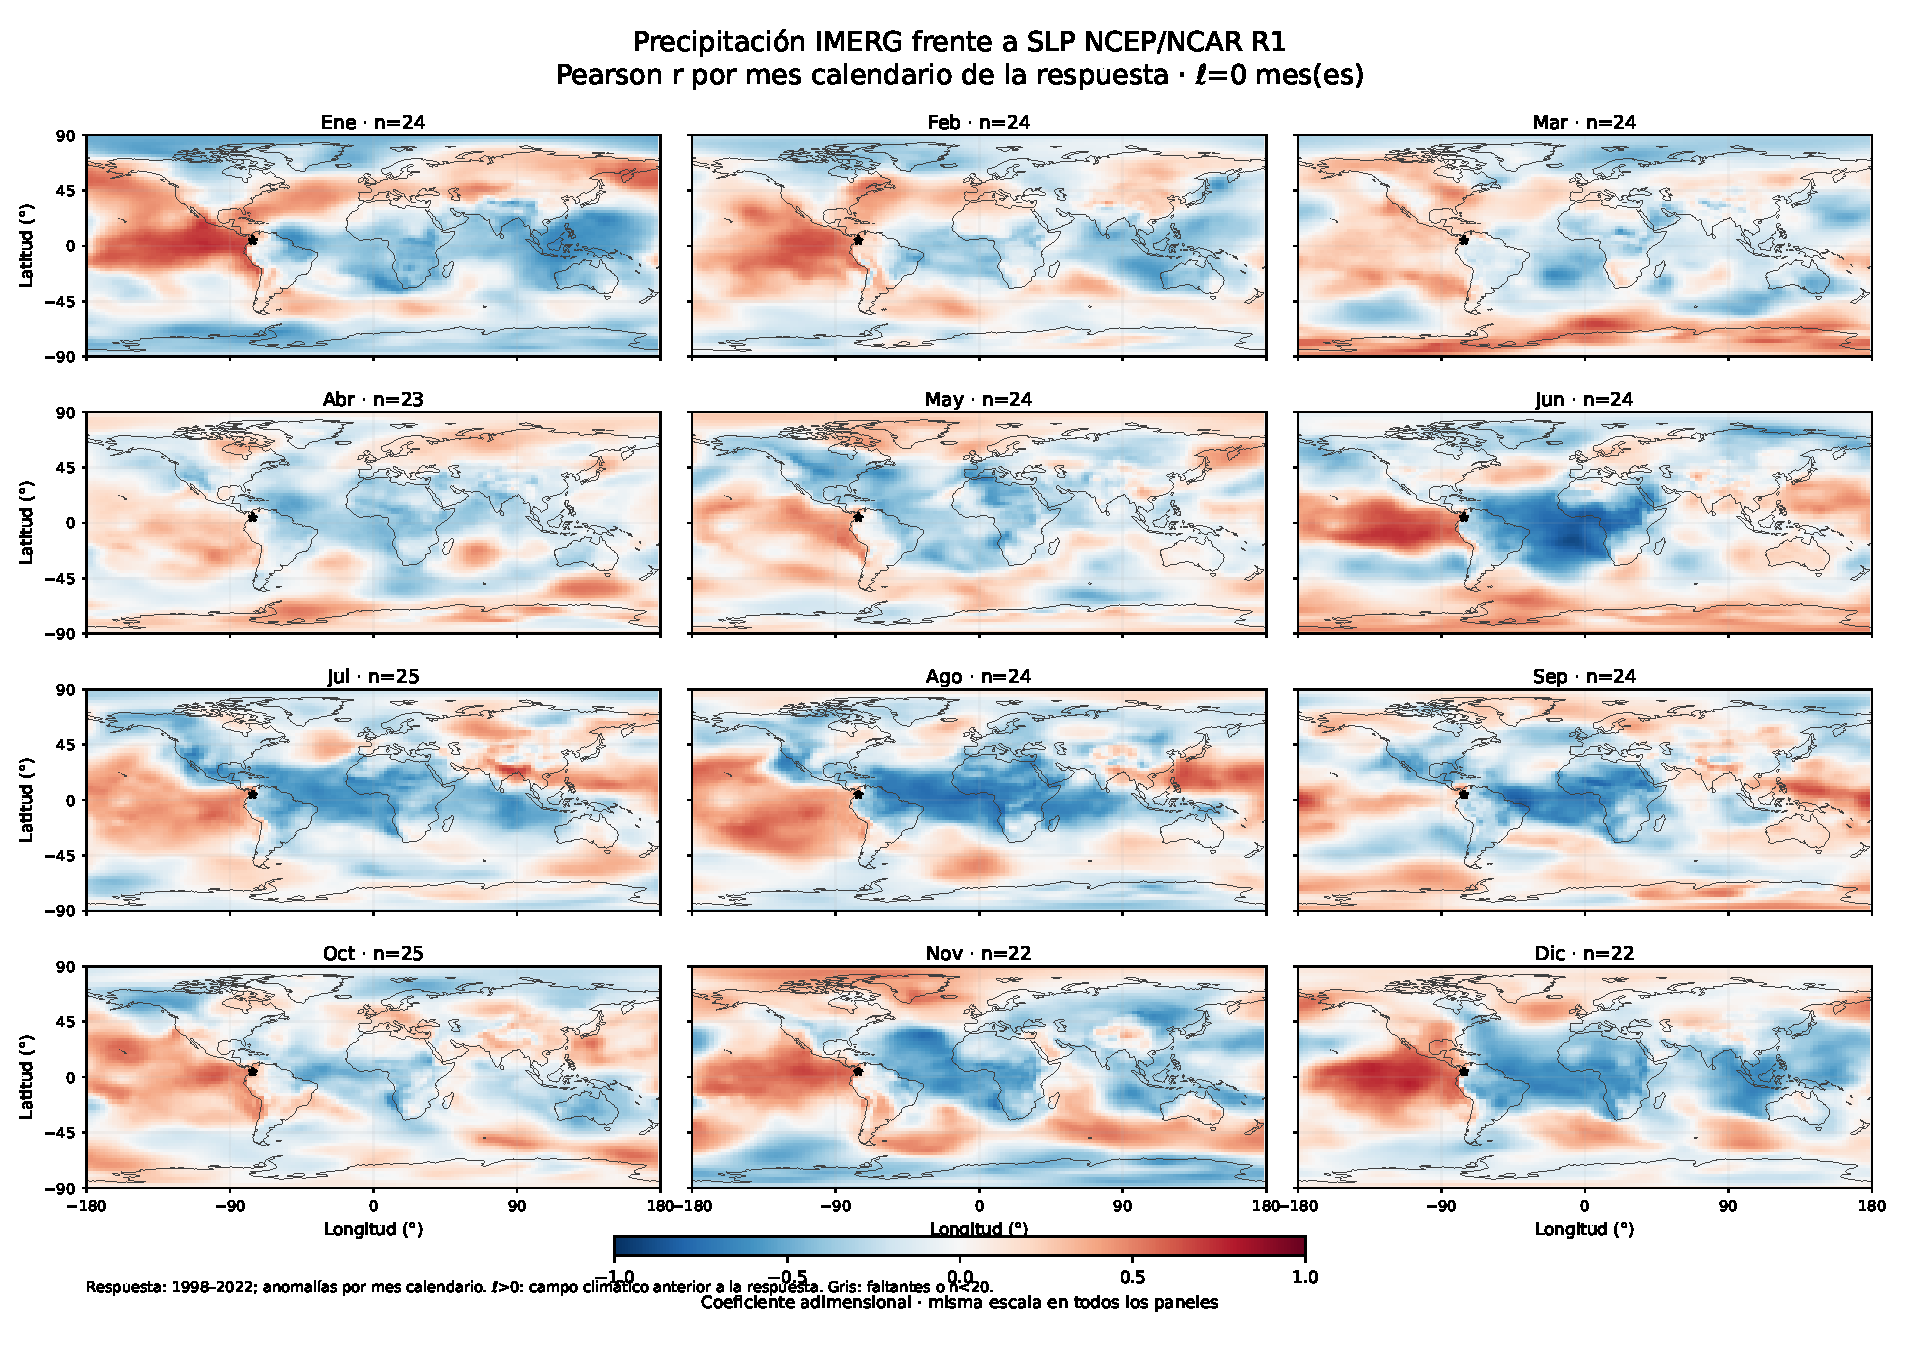
\includegraphics[width=\linewidth]{../apartado_5_2/IMERG_slp_l0_pearson.pdf}\caption{Doce correlaciones temporales por mes calendario; rezago 0 mes(es).}\end{figure}
\begin{figure}[p]\centering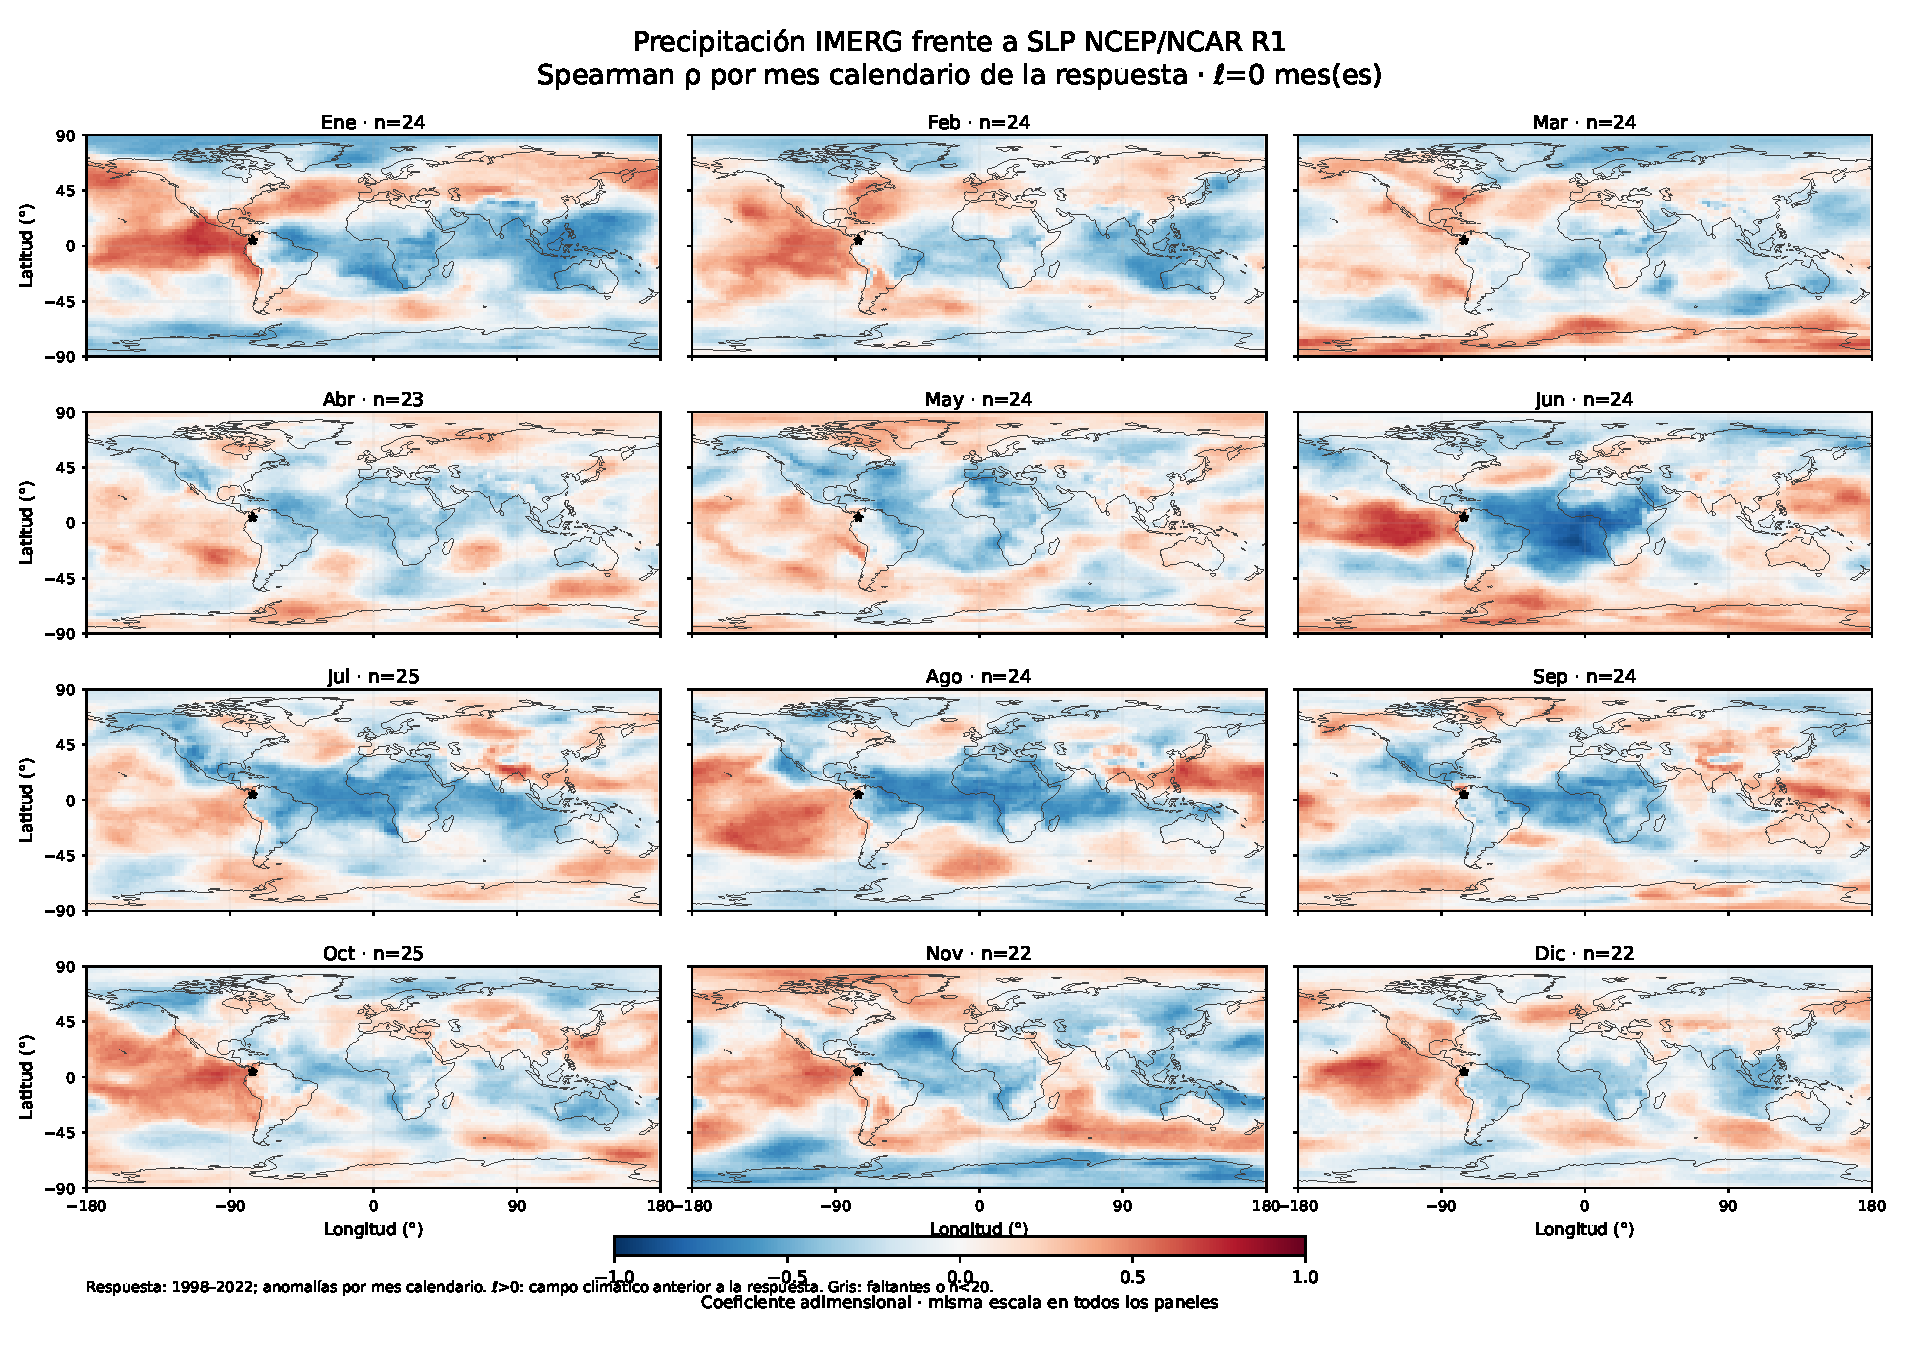
\includegraphics[width=\linewidth]{../apartado_5_2/IMERG_slp_l0_spearman.pdf}\caption{Doce correlaciones temporales por mes calendario; rezago 0 mes(es).}\end{figure}
\begin{figure}[p]\centering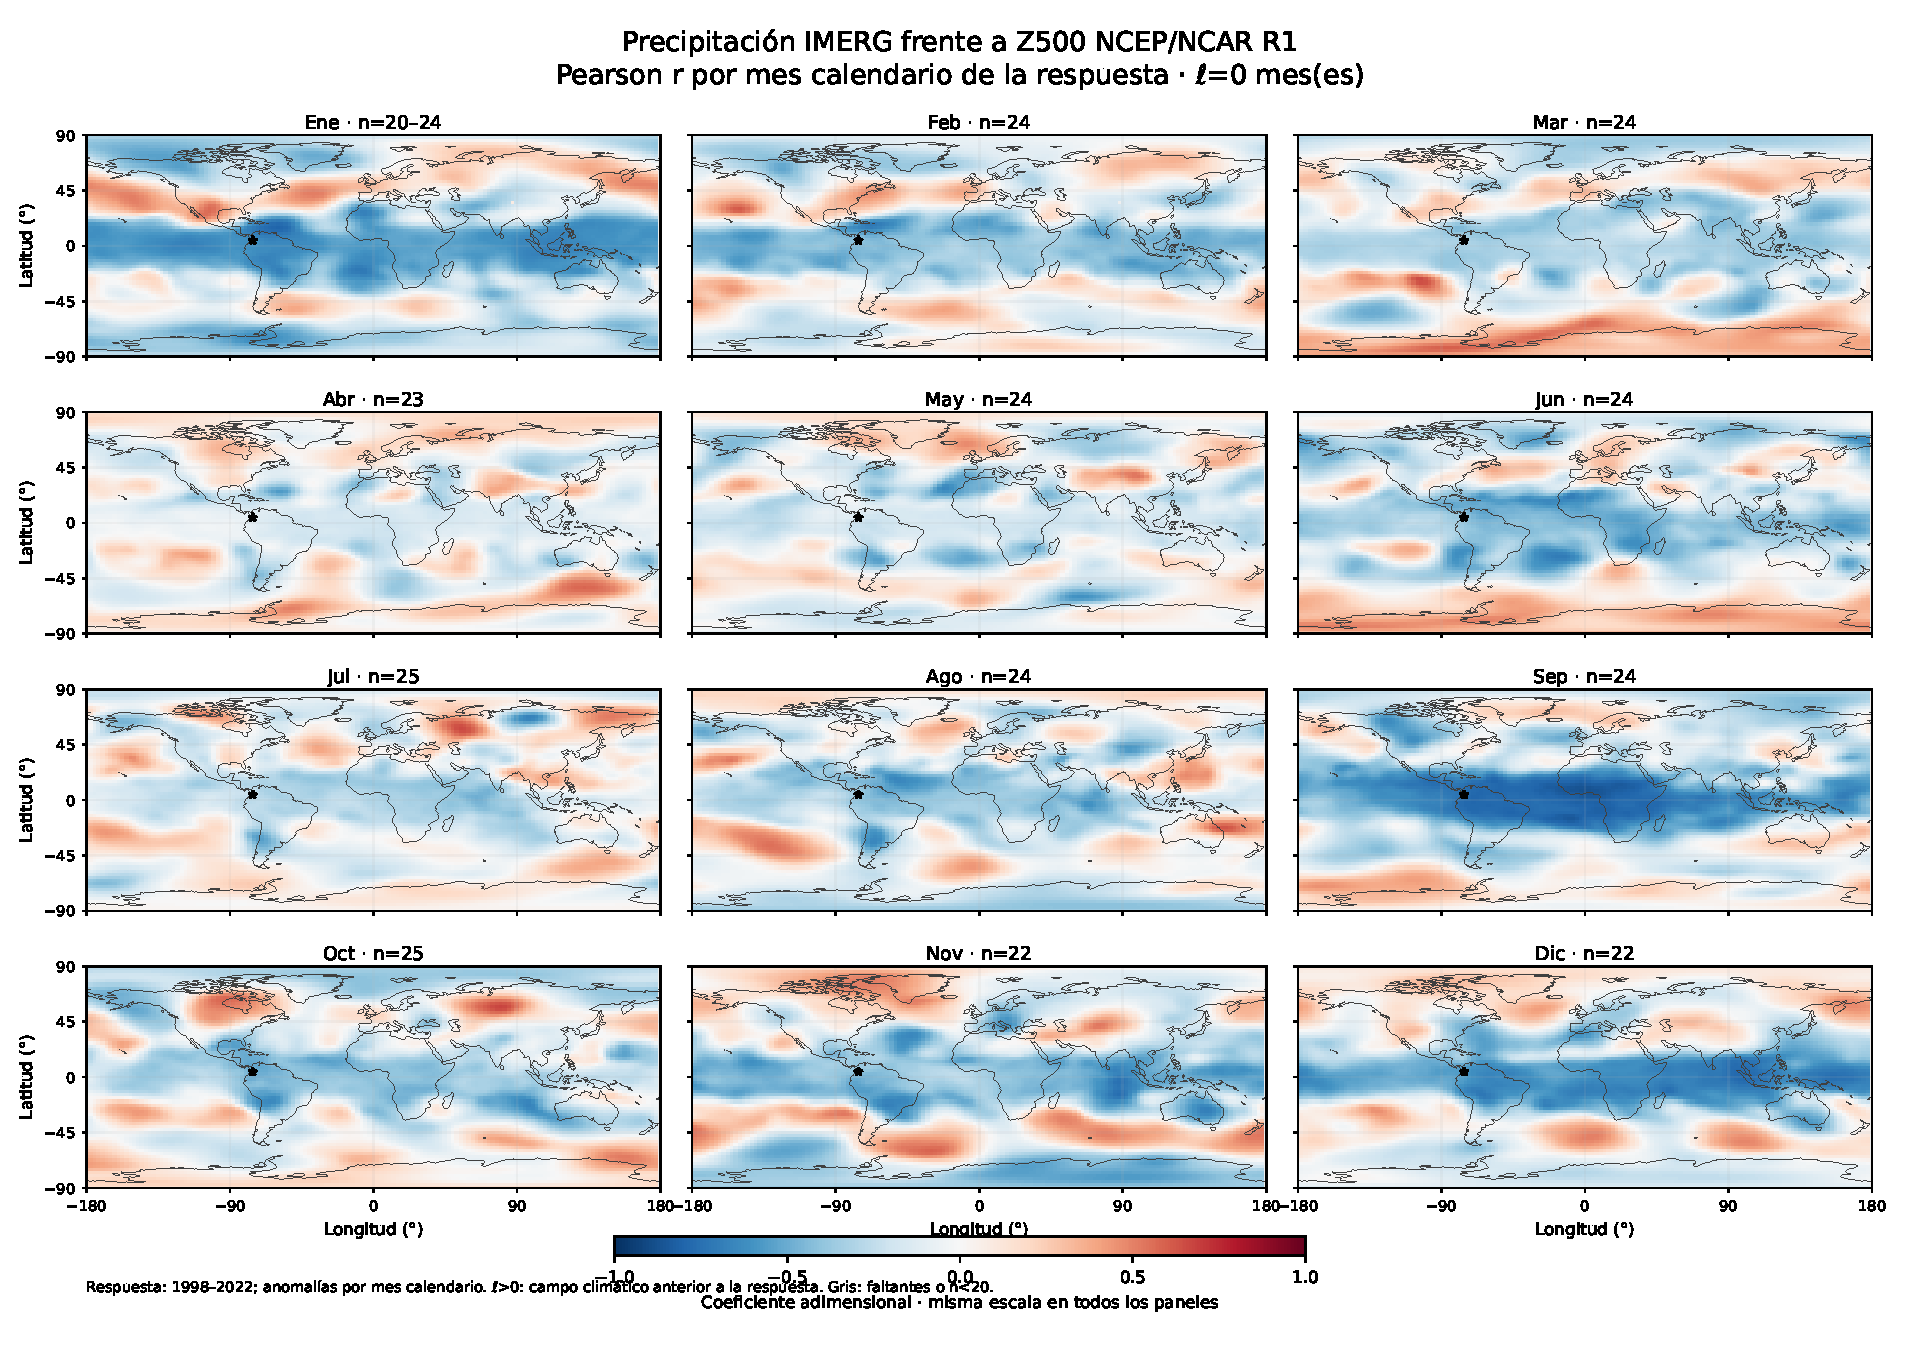
\includegraphics[width=\linewidth]{../apartado_5_2/IMERG_z500_l0_pearson.pdf}\caption{Doce correlaciones temporales por mes calendario; rezago 0 mes(es).}\end{figure}
\begin{figure}[p]\centering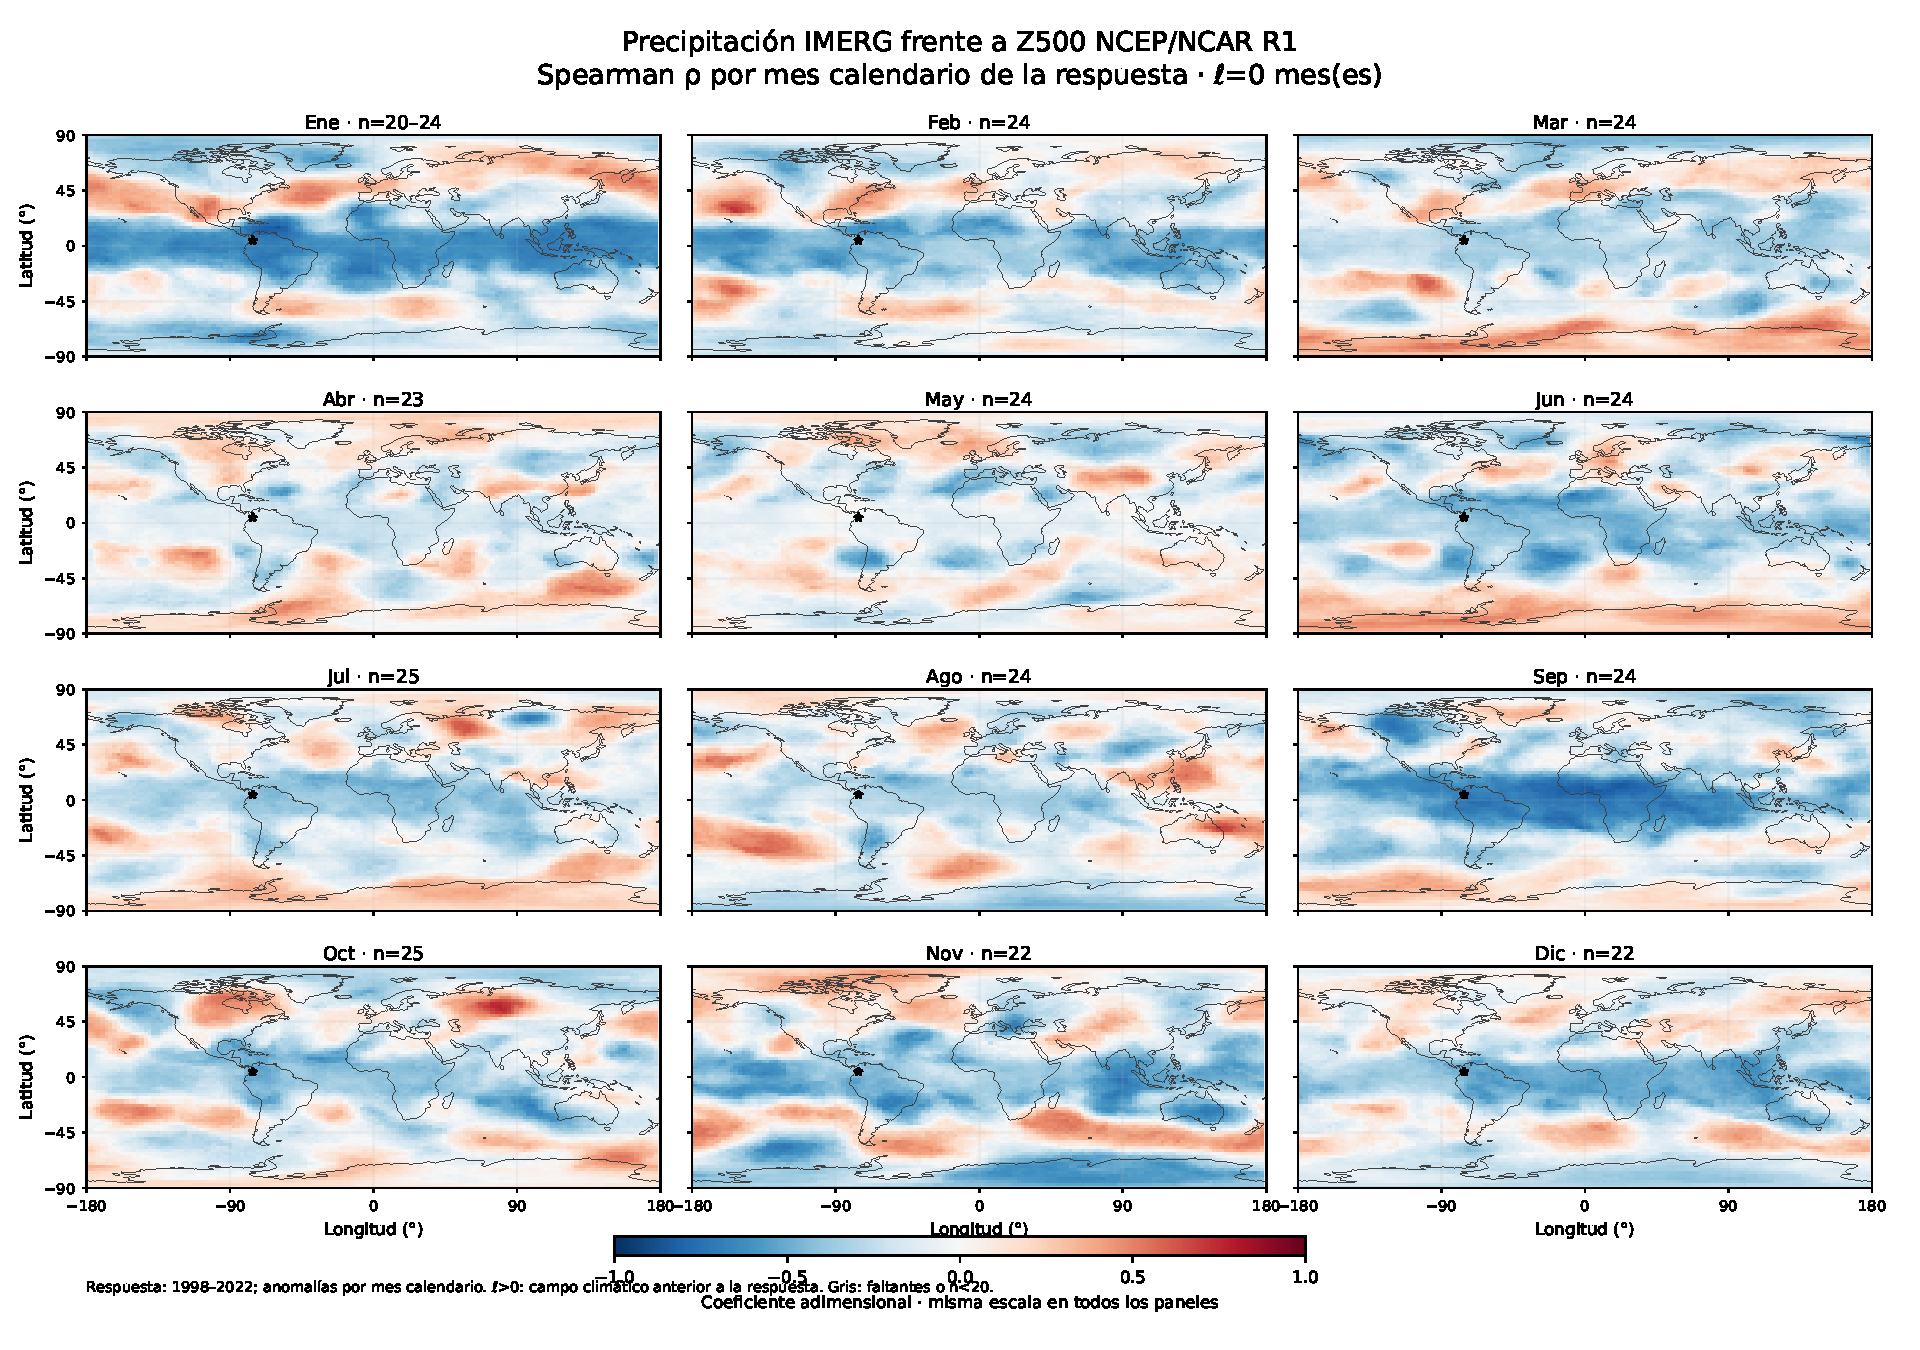
\includegraphics[width=\linewidth]{../apartado_5_2/IMERG_z500_l0_spearman.pdf}\caption{Doce correlaciones temporales por mes calendario; rezago 0 mes(es).}\end{figure}
\subsection{Robustez y presentación de los patrones}
Pendiente de desarrollar.
\subsection{Interpretación física e integración}
Pendiente de desarrollar.
\section*{Conclusiones}
Pendiente de síntesis final.

\section*{Procedencia, alcance y reproducibilidad}
\subsubsection*{Procedencia y alcance}
\subsubsection*{Procedencia de los datos}
Se utiliza CAMELS-COL, depósito del 26 de febrero de 2026, DOI
\href{https://doi.org/10.5281/zenodo.18794895}{10.5281/zenodo.18794895}, consultado
el 21 de septiembre de 2026. El archivo de entrada es
\path{Hydromet_data_26127040.txt}, incluido en
\path{04_CAMELS_COL_Hydrometeorological_data.zip}, para la cuenca del río
La Vieja hasta la estación Cartago (IDEAM 26127040).
\begin{itemize}
\item \textbf{Precipitación:} CHIRPS v2, datos diarios promediados sobre la cuenca
por los autores de CAMELS-COL, en mm/día. Es un producto combinado, no una
medición directa de un único pluviómetro.
\item \textbf{Caudal:} valores diarios reportados como observados en la estación
hidrométrica IDEAM, distribuidos mediante CAMELS-COL, en m$^3$/s. No se
descargaron aforos originales directamente del IDEAM.
\item \textbf{Área y delimitación:} atributos y polígono CAMELS-COL; área
reportada de 2797,19 km$^2$. Nombre y ubicación contrastados con el catálogo IDEAM.
\item \textbf{Temperatura:} el archivo contiene Tmin y Tmax de MSWX; se grafican sus medias mensuales y una Tmedia estimada como $(Tmin+Tmax)/2$, no una media horaria observada.
\end{itemize}

\subsubsection*{Alcance temporal y procesamiento}
Se analiza enero de 1981 a diciembre de 2022 (42 años). Se reconstruyó el
calendario diario y se conservaron solo meses con el 100\,\% de días válidos:
485 de 504 meses. P mensual es la suma de P diaria; Q mensual es la media de Q
diaria. No se rellenaron faltantes, no se prorratearon sumas ni se eliminaron
extremos por su magnitud.

Las estadísticas globales y por año describen valores mensuales válidos. Mínimo
y máximo no son extremos instantáneos ni diarios. La desviación estándar es
muestral. Los años incompletos describen únicamente su muestra disponible.

\subsubsection*{Limitaciones y trabajo pendiente}
Este documento es una exploración descriptiva inicial. La cartografía de relieve utiliza Copernicus GLO-30, documentado en la sección de mapas. Las gráficas no prueban
tendencias, causalidad ni capacidad predictiva. No se ha certificado la
homogeneidad del registro, la ausencia de reconstrucciones previas o el efecto de
extracciones y regulación. No hay banderas por observación en el archivo diario
que permitan resolver esas cuestiones.

\textbf{IMERG está incorporado como promedio de caja para 1998--2022:} falta
calcular el promedio exacto ponderado por fracción de área del polígono y validar
los valores por celda. También quedan pendientes una temperatura media de fuente
directa y los registros individuales de estaciones de lluvia. El conteo de estaciones
no demuestra continuidad de sus series ni significa que se hayan utilizado como datos de entrada.

\subsubsection*{Reproducibilidad y apoyo de IA}
Los scripts numerados se conservan en \path{seleccion_cuenca/scripts/}.
La tabla común a las gráficas es \path{datos_graficados.csv};
\path{proveniencia.json} registra su huella SHA-256 y versiones de bibliotecas.
Las comprobaciones e intermedios están en \path{la_vieja/punto_1/}.
La IA apoyó la programación, la revisión aritmética y la redacción preliminar;
el grupo debe revisar fuentes, decisiones e interpretación.

PDF y HTML representan los mismos datos. El HTML incluye Plotly y las series y
funciona sin servidor ni Internet; consultar fuentes externas sí requiere conexión.

\section*{Uso de IA}
La declaración existente se conserva en el apartado anterior; falta completar la declaración final del grupo.
\section*{Referencias y anexos}
Las referencias y fuentes existentes se conservan junto a sus análisis; falta consolidar el listado final.
\end{document}
